%%%%%%%%%%%%%%%%%%%%%%%%%%%%%%%%%%%%%%%%%%%%%%%%%%%%%%%%%%%%%%%%%%%%%%%%%%%%%%%%
%                         FORMATO DE TESIS UMSNH                               %
%%%%%%%%%%%%%%%%%%%%%%%%%%%%%%%%%%%%%%%%%%%%%%%%%%%%%%%%%%%%%%%%%%%%%%%%%%%%%%%%
% based on Harish Bhanderi's PhD/MPhil template, then Uni Cambridge
% http://www-h.eng.cam.ac.uk/help/tpl/textprocessing/ThesisStyle/
% corrected and extended in 2007 by Jakob Suckale, then MPI-iCBG PhD programme
% and made available through OpenWetWare.org - the free biology wiki
% forked from https://github.com/Tepexic/Tesis-UNAM on July 2017
% modifications made by Arturo Lopez Pineda

% Modifications made by Elioth Monroy Martos (2018-2019)

%                     Under GNU License v3

% ADAPTADO PARA UMSNH:  @arturolp

% Adaptado para ESCOM-IPN: @EliothMonroy

\documentclass[oneside,11pt]{Latex/Classes/thesisUMSNH}
%         PUEDEN INCLUIR EN ESTE ESPACIO LOS PAQUETES EXTRA, O BIEN, EN EL ARCHIVO "PhDthesisPSnPDF.cls" EN "./Latex/Classes/"
%\usepackage{blindtext}                        % Para insertar texto dummy, de ejemplo, pues.
\usepackage[square, sort, numbers]{natbib}  % Personalizar la bibliografía a gusto de cada quien
% Note:
%\usepackage{enumerate}
\usepackage{enumitem}
\usepackage{hyperref}
\usepackage{array}
\newcolumntype{P}[1]{>{\centering\arraybackslash}p{#1}}
\newcolumntype{M}[1]{>{\centering\arraybackslash}m{#1}} %Centra tanto vertical como horizontalmente
\newcolumntype{J}[1]{>{\arraybackslash}m{#1}} % Justifica el contenido dentro de una tabla y centra verticalmente
\usepackage{longtable}
\usepackage{graphicx}
\usepackage{verbatim}
% The \blindtext or \Blindtext commands throughout this template generate dummy text
% to fill the template out. These commands should all be removed when 
% writing thesis content.
% This file contains macros that can be called up from connected TeX files
% It helps to summarise repeated code, e.g. figure insertion (see below).

%%%%%%%%%%%%%%%%%%%%%%%%%%%%%%%%%%%%%%%%%%%%%%
%            Colores de la UNAM              %
%%%%%%%%%%%%%%%%%%%%%%%%%%%%%%%%%%%%%%%%%%%%%%
% Para UNAN: Azul Pantone 541  -->(0,63,119) RGB
% Para UMSNH: PANTONE Blue 072 C
\definecolor{Azul}{RGB}{51,51,153}
\definecolor{Guinda}{RGB}{108,19,43}

% Para UNAM: Oro Pantone 460  -->(234,221,150) RGB
% Para UMNSH: PANTONE 110 C
\definecolor{Oro}{RGB}{204,153,51}


%%%%%%%%%%%%%%%%%%%%%%%%%%%%%%%%%%%%%%%%%%%%%%
%            Comandos para líneas            %
%%%%%%%%%%%%%%%%%%%%%%%%%%%%%%%%%%%%%%%%%%%%%%
%Se define un comando \colorvrule para hacer líneas verticales de color con 3 argumentos: color, ancho, alto
\newcommand{\colorvrule}[3]{
\begingroup\color{#1}\vrule width#2 height#3
\endgroup}

%Se define un comando \colorhrule para hacer líneas horizontales de color con 2 argumentos: color, ancho
\newcommand{\colorhrule}[2]{
\begingroup\color{#1}\hrule height#2
\endgroup}

%%%%%%%%%%%%%%%%%%%%%%%%%%%%%%%%%%%%%%%%%%%%%%
%          Comando para derivadas            %
%%%%%%%%%%%%%%%%%%%%%%%%%%%%%%%%%%%%%%%%%%%%%%
\newcommand{\derivada}[3][]{\ensuremath{\dfrac{\mbox{d}^{#1}#2}{\mbox{d}#3^{#1}}}} 
%primer argumento(opcional): orden de la derivada
%segundo argumento: función a derivar
%tercer argumento: variable respecto a la que se deriva


%%%%%%%%%%%%%%%%%%%%%%%%%%%%%%%%%%%%%%%%%%%%%%
%       Comando para la exponencial          %
%%%%%%%%%%%%%%%%%%%%%%%%%%%%%%%%%%%%%%%%%%%%%%
\newcommand{\e}[1][]{\ensuremath{\mbox{e}^{#1}}}
%primer argumento(opcional): exponente de la exponencial




% insert a centered figure with caption and description
% parameters 1:filename, 2:title, 3:description and label
\newcommand{\figuremacro}[3]{
	\begin{figure}[htbp]
		\centering
		\includegraphics[width=1\textwidth]{#1}
		\caption[#2]{\textbf{#2} - #3}
		\label{condicion}
	\end{figure}
}

% insert a centered figure with caption and description AND WIDTH
% parameters 1:filename, 2:title, 3:description and label, 4: textwidth
% textwidth 1 means as text, 0.5 means half the width of the text
\newcommand{\figuremacroW}[4]{
	\begin{figure}[htbp]
		\centering
		\includegraphics[width=#4\textwidth]{#1}
		\caption[#2]{\textbf{#2} - #3}
		\label{#1}
	\end{figure}
}

% inserts a figure with wrapped around text; only suitable for NARROW figs
% o is for outside on a double paged document; others: l, r, i(inside)
% text and figure will each be half of the document width
% note: long captions often crash with adjacent content; take care
% in general: above 2 macro produce more reliable layout
\newcommand{\figuremacroN}[3]{
	\begin{wrapfigure}{o}{0.5\textwidth}
		\centering
		\includegraphics[width=0.48\textwidth]{#1}
		\caption[#2]{{\small\textbf{#2} - #3}}
		\label{#1}
	\end{wrapfigure}
}

% predefined commands by Harish
\newcommand{\PdfPsText}[2]{
  \ifpdf
     #1
  \else
     #2
  \fi
}

\newcommand{\IncludeGraphicsH}[3]{
  \PdfPsText{\includegraphics[height=#2]{#1}}{\includegraphics[bb = #3, height=#2]{#1}}
}

\newcommand{\IncludeGraphicsW}[3]{
  \PdfPsText{\includegraphics[width=#2]{#1}}{\includegraphics[bb = #3, width=#2]{#1}}
}

\newcommand{\InsertFig}[3]{
  \begin{figure}[!htbp]
    \begin{center}
      \leavevmode
      #1
      \caption{#2}
      \label{#3}
    \end{center}
  \end{figure}
}







%%% Local Variables:
%%% mode: latex
%%% TeX-master: "~/Documents/LaTeX/CUEDThesisPSnPDF/thesis"
%%% End:
           % Archivo con funciones útiles





%%%%%%%%%%%%%%%%%%%%%%%%%%%%%%%%%%%%%%%%%%%%%%%%%%%%%%%%%%%%%%%%%%%%%%%%%%%%%%%%
%                                   DATOS                                      %
%%%%%%%%%%%%%%%%%%%%%%%%%%%%%%%%%%%%%%%%%%%%%%%%%%%%%%%%%%%%%%%%%%%%%%%%%%%%%%%%
\title{Prototipo de aplicación móvil para el reporte y medición de la cantidad de combustible que se suministra a un automóvil    YA PÁRALE ANDRES SON VACACIONES x2, REGRESAMOS EL 7 DE ENERO BANDA}
\author{Saldaña Aguilar Andrés Arnulfo \\Arteaga Lara Samuel de Barca\\Flores Tepatl Giselle} 
\facultad{Escuela Superior de Cómputo}                 % Nombre de la facultad/escuela
% \escudofacultad{Latex/Classes/Escudos/fmed_grande} % Aquí ponen la ruta y nombre del escudo de su facultad.

\degree{Ingeniería en Sistemas Computacionales}       % Carrera
\director{M. en C. Víctor Hugo García Ortega \quad \quad \quad Dr. Rubén Ortega González}     % Directores de tesis
%\tutor{Nombre  Tutor }                    % Tutor de tesis, si aplica
\degreedate{6 de Noviembre del 2018}            % Año de la fecha de la presentación
\lugar{Ciudad de México}                        % Lugar

%\portadafalse                              % Portada en NEGRO, descomentar y comentar la línea siguiente si se quiere utilizar
\portadatrue                                % Portada en COLOR



%% Opciones del posgrado (descomentar si las necesitan)
	%\posgradotrue                                                    
	%\programa{programa de maestría y doctorado en ingeniería}
	%\campo{Ingeniería Eléctrica - Control}
	%% En caso de que haya comité tutor
	%\comitetrue
	%\ctutoruno{Dr. Emmet L. Brown}
	%\ctutordos{Dr. El Doctor}
%% Datos del jurado                             
	%\presidente{Dr. 1}
	%\secretario{Dr. 2}
	%\vocal{Dr. 3}
	%\supuno{Dr. 4}
	%\supdos{Dr. 5}
	%\institucion{el Instituto de Ingeniería, UNAM}

\keywords{gasolina,trabajo terminal}            % Palablas clave para los metadatos del PDF
\subject{tema_1,tema_2}                     % Tema para metadatos del PDF  

%%%%%%%%%%%%%%%%%%%%%%%%%%%%%%%%%%%%%%%%%%%%%%%%%%%%%
%                   PORTADA                         %
%%%%%%%%%%%%%%%%%%%%%%%%%%%%%%%%%%%%%%%%%%%%%%%%%%%%%
\begin{document}

\maketitle	% Se redefinió este comando en el archivo de la clase para generar automáticamente la portada a partir de los datos

%%%%%%%%%%%%%%%%%%%%%%%%%%%%%%%%%%%%%%%%%%%%%%%%%%%%%
%                  PRÓLOGO                          %
%%%%%%%%%%%%%%%%%%%%%%%%%%%%%%%%%%%%%%%%%%%%%%%%%%%%%
\frontmatter
% \begin{dedication}
A la Facultad de Ingeniería y a la  Universidad, por la formación que me han dado.\\
Es gracias a ustedes que es posible el presente trabajo.\\
En verdad, gracias.\\
Yo.
\end{dedication}
       % Comentar línea si no se usa
% %\chapter*{}
%\pagenumbering{Roman}

\begin{acknowledgements}

Gracias al Instituto Politécnico Nacional, por habernos permitido formarnos como personas y profesionales, gracias a todas las personas que fueron participes de este proceso, ya sea de manera directa o indirecta fueron ustedes los responsables de realizar su aporte qué, el día de hoy se ve reflejado en la culminación de este trabajo terminal de manera exitosa. Gracias a nuestros padres, seres queridos, profesores y colegas de profesión e institución, que fueron nuestros mayores promotores y motivadores durante este proceso.
\\
\\
\textbf{La Técnica al Servicio de la Patria}

\end{acknowledgements}




   % Comentar línea si no se usa 
% % ******************************* Thesis Declaration ********************************

\begin{declaration}

Por la presente declaro que, salvo cuando se haga referencia específica al trabajo de otras personas, el contenido de esta tesis es original y no se ha presentado total o parcialmente para su consideración para cualquier otro título o grado en esta o cualquier otra Universidad. Esta tesis es resultado de mi propio trabajo y no incluye nada que sea el resultado de algún trabajo realizado en colaboración, salvo que se indique específicamente en el texto. 
% Author and date will be inserted automatically from thesis.tex


\end{declaration}
           % Comentar línea si no se usa
% 
% Thesis Abstract -----------------------------------------------------


%\begin{abstractslong}    %uncommenting this line, gives a different abstract heading
\begin{abstracts}        %this creates the heading for the abstract page

This is where you write your abstract ...
\blindtext

\end{abstracts}
%\end{abstractlongs}


% ----------------------------------------------------------------------                   % Comentar línea si no se usa

%%%%%%%%%%%%%%%%%%%%%%%%%%%%%%%%%%%%%%%%%%%%%%%%%%%%%
%                   ÍNDICES                         %
%%%%%%%%%%%%%%%%%%%%%%%%%%%%%%%%%%%%%%%%%%%%%%%%%%%%%
%Esta sección genera el índice
\setcounter{secnumdepth}{3} % organisational level that receives a numbers
\setcounter{tocdepth}{3}    % print table of contents for level 3
\tableofcontents            % Genera el índice 
%: ----------------------- list of figures/tables ------------------------
\listoffigures              % Genera el ínidce de figuras, comentar línea si no se usa
\listoftables               % Genera índice de tablas, comentar línea si no se usa


%%%%%%%%%%%%%%%%%%%%%%%%%%%%%%%%%%%%%%%%%%%%%%%%%%%%%
%                   CONTENIDO                       %
%%%%%%%%%%%%%%%%%%%%%%%%%%%%%%%%%%%%%%%%%%%%%%%%%%%%%
% the main text starts here with the introduction, 1st chapter,...
\mainmatter
\def\baselinestretch{1.5}                   % Interlineado de 1.5

% this file is called up by thesis.tex
% content in this file will be fed into the main document
%----------------------- introduction file header -----------------------
%%%%%%%%%%%%%%%%%%%%%%%%%%%%%%%%%%%%%%%%%%%%%%%%%%%%%%%%%%%%%%%%%%%%%%%%%
%  Capítulo 1: Introducción- DEFINIR OBJETIVOS DE LA TESIS              %
%%%%%%%%%%%%%%%%%%%%%%%%%%%%%%%%%%%%%%%%%%%%%%%%%%%%%%%%%%%%%%%%%%%%%%%%%

\chapter{Introducción}

%: ----------------------- HELP: latex document organisation
% the commands below help you to subdivide and organise your thesis
%    \chapter{}       = level 1, top level
%    \section{}       = level 2
%    \subsection{}    = level 3
%    \subsubsection{} = level 4
%Cuando se use input, se debe poner la ruta desde el documento principal (o sea tesis.tex)
%%%%%%%%%%%%%%%%%%%%%%%%%%%%%%%%%%%%%%%%%%%%%%%%%%%%%%%%%%%%%%%%%%%%%%%%%
%                           Presentación                                %
%%%%%%%%%%%%%%%%%%%%%%%%%%%%%%%%%%%%%%%%%%%%%%%%%%%%%%%%%%%%%%%%%%%%%%%%%

\section{Presentación} % section headings are printed smaller than chapter names
El suministro de gasolina es una actividad que se realiza diariamente en miles de gasolineras de todo México, esta actividad consiste en la transmisión de gasolina al contenedor de combustible de un automóvil a través de una máquina dispensadora, dicho dispositivo registra la cantidad de gasolina suministrada (medida en litros) y muestra el equivalente en pesos a pagar según el precio del litro gasolina.
Dicha actividad es de suma importancia, ya que gran parte de las actividades económicas y personales en nuestro país dependen del uso de un vehículo cuyo funcionamiento requiera algún tipo de combustible. El proceso de suministro de gasolina depende de diversos factores, como lo son una serie de dispositivos electrónicos y mecánicos conectados entre sí, además de la interacción con la persona despachadora de la gasolina, todos estos factores influyen en la precisión con la que los litros de gasolina son suministrados a un vehículo.
\paragraph{}
En los últimos años, la Profeco (Procuraduría Federeal del Consumidor) ha detectado nuevas modalidades para el robo de gasolina, la mayoría de estas, sucede durante el proceso de recarga o suministro de gasolina, lo cuál, muchas veces suele pasar como un fenómeno desapercibido para el usuario final. 
Este problema, cobra especial relevancia en un país de consumo elevado de gasolina como México. Petróleos Mexicanos (PEMEX) informó que durante el primer semestre del año 2016 el consumo de gasolina fue de 812 mil barriles por día. Lo anterior equivale a 129 millones de litros diarios, de los cuales, 78 por ciento corresponde al tipo Magna y 22 por ciento al tipo Premium, según explica dicho órgano en su cuenta oficial de Twitter \citep{Pre1}.
Las cifras anteriores ubican a México entre los primeros consumidores de gasolina a nivel mundial. Además, en el año 2014 México ocupo la cuarta posición a nivel mundial en consumo de gasolina al día, solo por debajo de Estados Unidos, Japón y Canadá \citep{Pre2}.
\paragraph{}
Otro factor importante en el consumo de gasolina es el precio, según el sitio Global Petrol Prices en el año 2018 México se encuentra entre los países latinoamericanos con los precios más elevados para el litro de gasolina ubicándose en 1.01 dólares por litro al término del primer semestre \citep{Pre3}.
\\
La estadística anterior cobra mayor relevancia cuándo se estudian los ingresos económicos del mexicano. Los mexicanos gastan en promedio un 3.38 por ciento de sus ingresos, unos 5 mil 336 pesos, en comprar 358.94 litros de gasolina al año, que es el promedio que utiliza un conductor en el país \citep{Pre4}.
\paragraph{}
Basándonos en las estadísticas mencionadas con anterioridad observamos que el consumo de gasolina en México es una actividad de suma importancia y que afecta en buena parte las economías de las familias mexicanas. Dada la importancia económica de esta actividad las gasolineras cuentan con mecanismos de revisión que corroboran que el suministro de gasolina se realice de manera correcta en las gasolineras de país. Lamentablemente, muchas irregularidades se han presentado en los últimos años en diversas gasolineras, la mayoría de ellas tiene que ver con la exactitud al momento de despechar litros de combustible.
\paragraph{}
Durante el 2014, la Procuraduría Federal del Consumidor –Profeco- revisó 1,792 gasolineras, de las cuales, el 56\% (1,017 estaciones) tuvieron alguna irregularidad. Esta cifra es sin contar a las 233 gasolineras que se negaron a ser verificadas y mejor pagaron la multa correspondiente.
En lo que va del año 2018, la Profeco ha revisado 400 estaciones de servicio, de las cuales 68\% (274 gasolineras) fueron inmovilizadas no sólo por no despachar completo sino por no contar con las señalizaciones adecuadas. Asimismo, 39 gasolineras se negaron a ser revisadas por lo que pagaron la multa de \$250,000 pesos \citep{Pre5}.
\paragraph{}
Actualmente, la Profeco posee una lista negra con las gasolineras en las que se han encontrado irregularidades, sin embargo, dicha lista es actualizada después del periodo de revisiones lo cuál decrementa la exactitud de la lista debido a un periodo largo de actualización, además, cómo ya se mencionó existen gasolineras que evitan una revisión mediante el pago de una multa, lo cuál impide que exista una clasificación correcta de las gasolineras.
\paragraph{}
La propuesta de solución planteada en este trabajo terminal consiste en la creación de una aplicación móvil que permita realizar una mejor clasificación de las gasolineras de acuerdo con su exactitud al momento de cargar gasolina. Dicha clasificación será actualizada constantemente con la ayuda de un sensor que medirá la cantidad de litros ingresados al vehículo, de esta forma, pondrán ser censadas todas aquellas gasolineras que evitan una revisión de la Profeco mediante el pago de una multa. Finalmente, la clasificación de las gasolineras no dependerá de una sola revisión, sino que será retroalimentada por las mediciones constantes de cada sensor presente en un automóvil al momento de cargar gasolina, lo cuál incrementa la exactitud en el algoritmo de clasificación.
%%%%%%%%%%%%%%%%%%%%%%%%%%%%%%%%%%%%%%%%%%%%%%%%%%%%%%%%%%%%%%%%%%%%%%%%%
%                           Motivación y estado del arte                %
%%%%%%%%%%%%%%%%%%%%%%%%%%%%%%%%%%%%%%%%%%%%%%%%%%%%%%%%%%%%%%%%%%%%%%%%%
\section{Justificación}
El incremento en el uso de fuentes de energía renovables en la actualidad tiene cada vez mayor relevancia debido a que en países como México, tiene un costo inferior de obtención que los combustibles fósiles \citep{Not1}, gracias al progreso que se ha logrado en este campo, la utilización de energía solar incrementó en un 13\% en México en el 2018 \citep{Not2}, siendo así la energía fotovoltaica una de las fuentes renovables más accesibles y eficientes para su aplicación en proyectos de pequeña o gran magnitud.
El presente trabajo terminal ofrece un sistema que permitirá a los usuarios de sistemas fotovoltaicos consultar y monitorear mediante una aplicación las variable de potencia activa para que estos tengan conocimiento de la producción de energía de la instalación.

%%%%%%%%%%%%%%%%%%%%%%%%%%%%%%%%%%%%%%%%%%%%%%%%%%%%%%%%%%%%%%%%%%%%%%%%%
%                   Planteamiento del problema                          %
%%%%%%%%%%%%%%%%%%%%%%%%%%%%%%%%%%%%%%%%%%%%%%%%%%%%%%%%%%%%%%%%%%%%%%%%%

\section{Planteamiento del problema}

La necesidad que atenderá la aplicación es monitorear el voltaje y corriente que se está generando a cada instante para que el usuario pueda consultar dicha información con el objeto de tener en continua observación los sistemas de generación de energía para atender los fallos, accidentes o anomalías que puedan afectar su correcto funcionamiento. Consiguiendo disminuir pérdidas cuando es una de las principales fuentes de abastecimiento y brindar un registro histórico de la producción de energía.


%%%%%%%%%%%%%%%%%%%%%%%%%%%%%%%%%%%%%%%%%%%%%%%%%%%%%%%%%%%%%%%%%%%%%%%%%
%                           Objetivo                                    %
%%%%%%%%%%%%%%%%%%%%%%%%%%%%%%%%%%%%%%%%%%%%%%%%%%%%%%%%%%%%%%%%%%%%%%%%%

\section{Objetivos}

\subsection{Objetivo general}
Este trabajo tiene por objetivo desarrollar un prototipo de sistema que permita monitorear el voltaje y la corriente de los usuarios de módulos de generación de energía fotovoltaica usando un sistema embebido para la recepción de la información recaudada por el sensor y el envió de estas para que la aplicación pueda desplegarla al usuario.

\subsection{Objetivos específicos}
\begin{enumerate}[label=\arabic*.]
    \item Implementar un nodo sensor que permita monitorear una fuente de energía fotovoltaica.
    \item Implementar el módulo para la transmisión de datos obtenidos por el sensor hacia el servidor, haciendo uso de un microcontrolador con módulo WiFi. 
    \item Desarrollar una aplicación que permita al usuario visualizar los datos obtenidos, resultado del monitoreo de la fuente de energía fotovoltaica.
    \item Documentar el trabajo realizado.
\end{enumerate}

%%%%%%%%%%%%%%%%%%%%%%%%%%%%%%%%%%%%%%%%%%%%%%%%%%%%%%%%%%%%%%%%%%%%%%%%%
%                           Estado del arte                              %
%%%%%%%%%%%%%%%%%%%%%%%%%%%%%%%%%%%%%%%%%%%%%%%%%%%%%%%%%%%%%%%%%%%%%%%%%
\section{Estado del arte}
Actualmente, existen interfaces que permiten la conexión e incorporación de diversas fuentes de generación de energía a la red eléctrica, a tales interfaces se les conoce con el nombre de microrredes \citep{Microrredes}. Este nuevo esquema de generación se caracteriza por la flexibilidad y autonomía con la que operan estas microrredes. Es decir, que, en caso de fallos de la red de distribución, estas puedan proporcionar energía directamente al usuario, siendo con esto más flexibles que los esquemas de distribución de energía ya existentes.\\

Para realizar el monitoreo de las microrredes se pueden emplear tecnologías de comunicación alámbricas e inalámbricas. En la división de tecnologías inalámbricas se encuentran las redes de sensores inalámbricas (WSN – Wireless Sensor Network).\\

Una WSN consiste en nodos de sensores autónomos implementados en zonas de interés que tienen en común características como:
\begin{itemize}
	\item Procesamiento de datos
	\item Capacidad de almacenamiento
	\item Interfaces de comunicación inalámbrica
	\item Consumo de energía limitada
\end{itemize}

Estos nodos sensores son un sistema computacional diseñado con hardware y software especialmente para realizar tareas específicas logrando así obtener beneficios en desempeño, costo y usabilidad del sistema, por lo que se le denomina un sistema embebido \citep{SistemaEmbebido}. A continuación, se hace mención de algunos de los trabajos de investigación que hacen referencia al uso de estas tecnologías:\\

\begin{itemize}
	\item En \citep{EstadoDelArte1} se propone el monitoreo autónomo de voltaje y corriente con el propósito de alertar fallas de cortocircuito, descargas o sobrealimentación de voltaje, también tiene la capacidad de controlar circuitos de protección cuando estas fallas acontezcan, esto es logrado colocando transductores (en este caso, sensores de efecto Hall) en las áreas de interés de la microrred , el acondicionamiento de la señal y procesamiento están a cargo de un microcontrolador, el envío de los datos adquiridos por medio de un arduino uno y un módulo de internet y finalmente enviando los datos a la plataforma de IoT Ubidots. 

    \item En \citep{EstadoDelArte2} se propone el monitoreo y control de una microrred simulada, donde el modelo de microrred es simulado por medio de MATLAB en una computadora que solo tendrá esa tarea, se ocupa un DAQ (Acondicionador de señales  y convertidor Analógico-Digital) para obtener los datos generados y son enviados a un PLC (Controlador Lógico Programable) que está conectado al DAQ, este se encarga de guardar y escanear continuamente las variables de la microrred para ser monitoreadas en el sistema SCADA (Supervisión, Control y Adquisición de Datos) Honeywell Experion PKS.

    \item En \citep{EstadoDelArte3} se propone un sistema de gestión de microrredes basado en WiFi, donde el sistema de control y sensado de la microrred es manejado por un software ya existente y sensores de potencia eléctrica (en conjunto denominado como Dispositivo de control) que está conectado por medio de un cable ethernet a un módulo inalámbrico que enviará los datos a un Router que se encargará de capturar los datos de los módulos conectados a la WLAN (Red de Área Local Inalámbrica) para que el servidor los almacene en la base de datos y puedan ser accedidos posteriormente. 

    \item En \citep{EstadoDelArte4} el sistema de control y monitoreo propuesto, está conformado por un subsistema capaz de monitorear hasta 18 circuitos sobre un rango de voltajes y corrientes, y es capaz de almacenar la información de manera interna o bien cargarla a un servidor remoto. Cabe señalar que el almacenamiento de la información se realiza en intervalos de 5 minutos en un archivo CSV, el cual es enviado a través de HTTP Push a una Raspberry Pi la cual tiene la función de controlador principal. A su vez, en la Raspberry Pi se ejecuta Tornado, un programa de servidor web que implementa la API Restful, de esta forma es como se acepta la información recolectada de los sensores, así como hacer llamadas RESTful para comunicarse con el resto de la arquitectura.
\end{itemize}
%%%%%%%%%%%%%%%%%%%%%%%%%%%%%%%%%%%%%%%%%%%%%%%%%%%%%%%%%%%%%%%%%%%%%%%%%
%                    Descripción del documento                           %
%%%%%%%%%%%%%%%%%%%%%%%%%%%%%%%%%%%%%%%%%%%%%%%%%%%%%%%%%%%%%%%%%%%%%%%%%
\section{Resumen}
El Sistema descrito y diseñado a continuación tiene como objetivo el monitoreo de la generación de energía de un Sistema fotovoltaico mediante el desarrollo de: un módulo de monitoreo que internamente está conformado por el dispositivo de sensado, el cual se comunica a su vez con el microcontrolador; un sistema embebido que permitirá el procesamiento y almacenamiento de la información monitoreada y una aplicación móvil que permita mantener informado al usuario sobre el estado del Sistema fotovoltaico, bajo el concepto del internet de las cosas, que se refiere a una interconexión digital de objetos cotidianos con Internet.

\section{Palabras clave}
Sistema embebido, IoT, Sistema Fotovoltaico, Nodo sensor, Red de sensores.

\section{Descripción del documento}
Este documento contiene la terminología y conceptos fundamentales tomados como base del presente trabajo terminal, para después hacer una descripción detallada del análisis y diseño. 
\\
En los capítulos siguientes se expresará a mayor profundidad el Trabajo Terminal, en el \textit{Capítulo \ref{chapter2} Marco conceptual} se presenta una referencia general, al ámbito bajo el cual es desarrollado el sistema, dando así, una introducción a los temas que son de interés para la correcta compresión de las diversas temáticas que abarca el Trabajo Terminal.
\\
En el \textit{Capítulo \ref{chapter3} Análisis del sistema} se redactan los distintos factores tomados en cuenta para la selección de tecnología, se explican los motivos por los cuales fueron usados ciertos dispositivos de hardware y tecnologías.
\\
En el \textit{Capítulo \ref{chapter4} Diseño del sistema}, se presenta el Diagrama del proceso general del Sistema, el cual informa sobre el flujo entre las tareas que se llevarán acabo dentro de él; también se incluyen los Modelos de información del Sistema que se realizarán para el almacenamiento de la información en el Sistema embebido así como el almacenamiento en la Aplicación de usuario; se presenta el diagrama de Hardware respecto a la parte que comprende el módulo de monitoreo del Sistema. Finalmente se incluye el diseño de los submódulos de monitoreo y de usuario para la parte de software, en el que se muestran los diagramas UML que permiten la construcción del sistema, mediante los diagramas de casos de uso.
\\
En el \textit{Capítulo \ref{chapter5} Conclusiones}, 
se realiza un resumen de los puntos más relevantes que fueron expuestos en cada uno de los capítulos del presente documento como resultado de la investigación, el análisis y el diseño del Sistema que será desarrollado.   
\\
En el \textit{Capítulo \ref{chapter6} Trabajo futuro}, se describirán los avances que tenemos programados para la segunda etapa del Trabajo Terminal.



%%%%%%%%%%%%%%%%%%%%%%%%%%%%%%%%%%%%%%%%%%%%%%%%%%%%%%%%%%%%%%%%%%%%%%%%%
%                           Marco Conceptual                               %
%%%%%%%%%%%%%%%%%%%%%%%%%%%%%%%%%%%%%%%%%%%%%%%%%%%%%%%%%%%%%%%%%%%%%%%%%

\chapter{Marco conceptual}\label{chapter2}

Dado que este trabajo terminal emplea conceptos de diversas áreas de la Ingeniería en Sistemas Computacionales, resulta fundamental abordar una serie de definiciones previas que permitirán un mejor entendimiento del documento.


\section{Sistema Fotovoltaico}
Un sistema fotovoltaico es un conjunto de dispositivos que aprovechan la energía producida por el Sol y la convierten en energía eléctrica \citep{MarcoTeorico1}. Un sistema fotovoltaico puede ser “interconectado” para residencias o negocios con acceso a la red eléctrica. 

\paragraph{}
Con este sistema la energía generada se inyecta a la red eléctrica, disminuyendo así el consumo de energía de la compañía de luz. La otra opción es un sistema “isla” que permite el suministro de energía eléctrica en lugares inaccesibles para la red eléctrica. Estos sistemas son usados principalmente en casas de campo o en antenas de telecomunicación.
\paragraph{}
La particularidad de la corriente eléctrica generada por el efecto fotovoltaico es que esta corriente es continua, por lo cual el inversor transforma la corriente continua en alterna al estándar de la Norma Oficial Mexicana NOM-001-SEDE-2012 de Instalaciones Eléctricas (127 Volts a 60 Hertz) \citep{NORMA-Electrica} para ser alimentada a la red eléctrica, en la figura \ref{fig:sistema fotovoltaicoa IUSA} se muestra la típica configuración de un sistema fotovoltaico:

\begin{figure}[H]
	\centering
	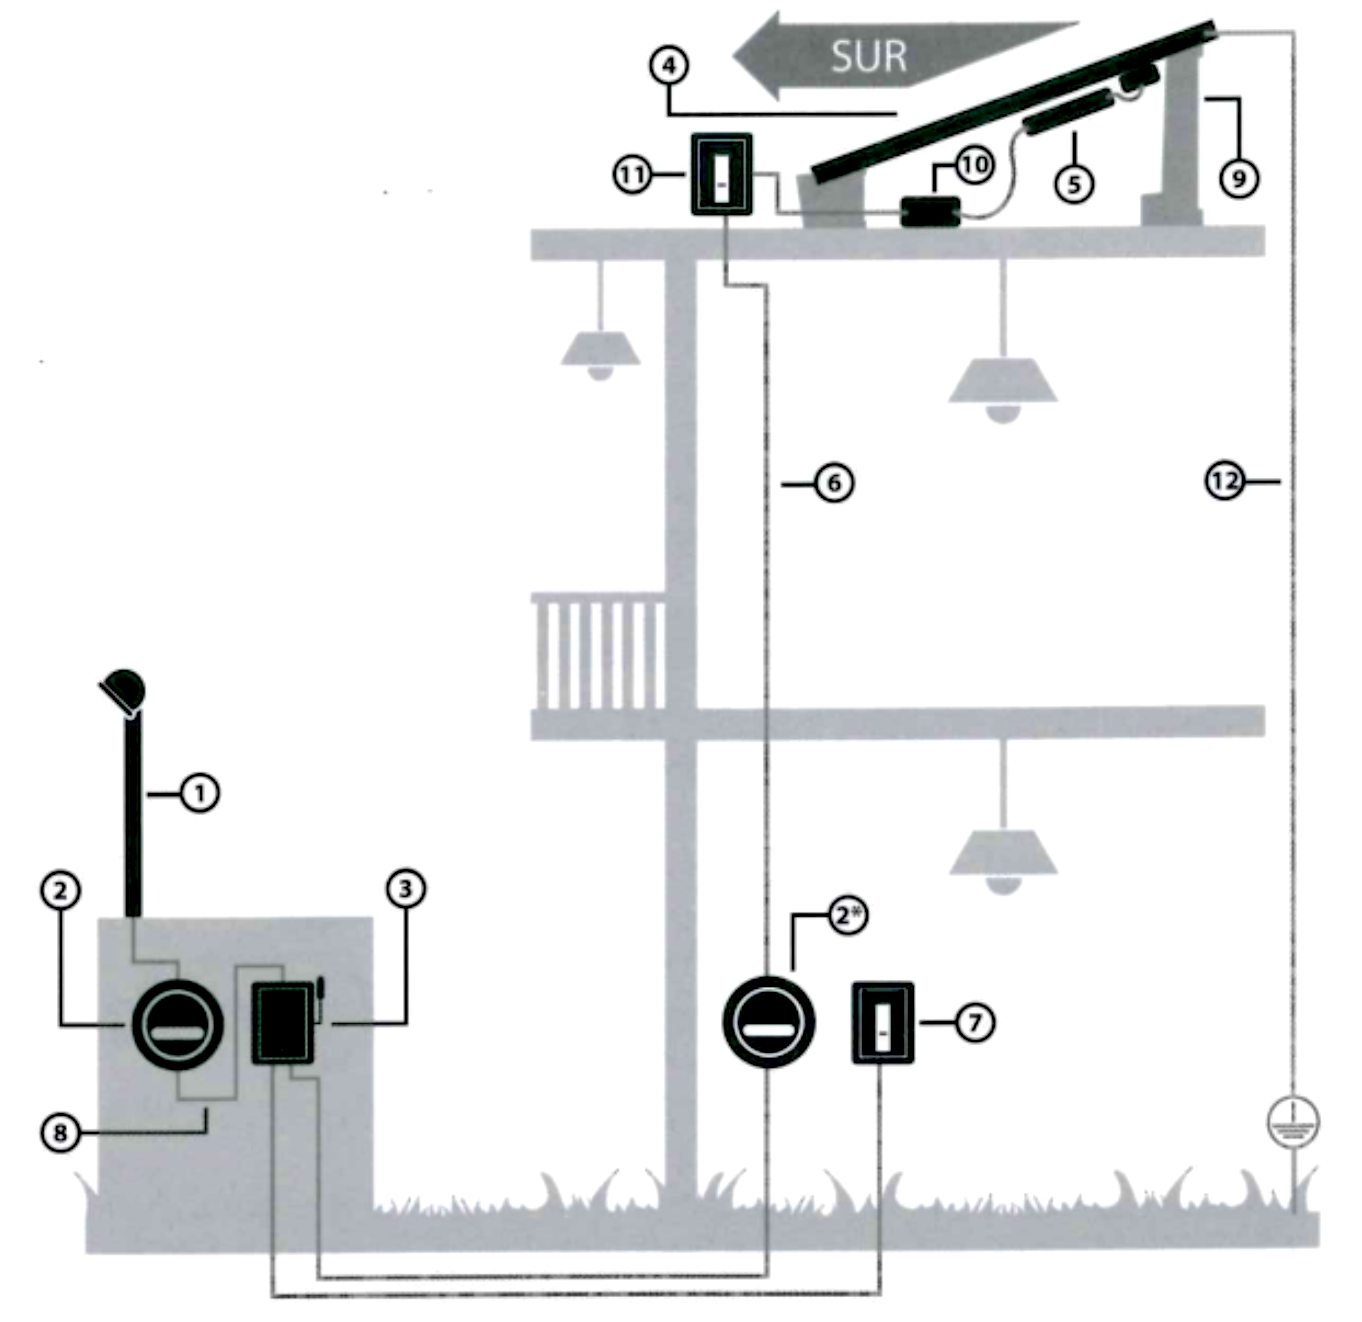
\includegraphics[scale=.4]{Capitulo2/images/sistema-fotovoltaico.png}
	\caption{Sistema Fotovoltaico Propuesto por el Fabricante IUSA}
	\label{fig:sistema fotovoltaicoa IUSA}
\end{figure}

Simbología y componentes básicos:
\begin{itemize}
	\item 1. Acometida
	\item 2. Medidor Bidireccional IUSA
	\item 2* Medidor Bidireccional IUSA (opcional)
	\item 3. Interruptor principal
	\item 4. Módulo fotovoltaico policristalino de 250 W
	\item 5. Microinversor C.D a C.A IUSA
	\item 6. Alimentador del sistema fotovoltaico
	\item 7. Tablero de distribución existente
	\item 8. Instalación eléctrica existente
	\item 9. Bases de madera sintética
	\item 10. Caja plexo
	\item 11. Interruptor del sistema fotovoltaico
	\item 12. Protección a tierra
\end{itemize}

\paragraph{Ley para el Aprovechamiento de Energías Renovables}
Las fuentes de energía renovables y las tecnologías limpias para generar electricidad se convierten en parte medular de un proceso de transición energética con la publicación de la
Ley para el Aprovechamiento de Energías Renovables y el Financiamiento de la Transición
Energética el 28 de noviembre de 2008, así como el Reglamento de la citada Ley el 2 de septiembre de 2009, además se resalta la importancia de establecer un programa de normalización en la
materia, que provea de las regulaciones y normas necesarias \citep{LeyAprovechamiento}.



\paragraph{NMX-J-643/1}
Esta Norma Mexicana establece los procedimientos para la medición de las
características corriente-tensión de dispositivos fotovoltaicos,
con luz solar natural o con un simulador solar. Estos
procedimientos son aplicables a una celda solar fotovoltaica
individual o un conjunto ensamblado de celdas solares
fotovoltaicas que forman un módulo fotovoltaico \citep{NMX-J-643/1}.

\paragraph{NMX-J-618/1}
Establece los requisitos de construcción para módulos fotovoltaicos (FV), con la finalidad de proporcionar operación mecánica y eléctrica segura, durante su vida útil. Se mencionan recomendaciones específicas para la prevención de choque eléctrico, riesgo de incendio y lesiones personales, que se originan por esfuerzos mecánicos y ambientales \citep{NMX-J-618/1}.

\paragraph{Contrato de interconexión para paneles solares}

Una vez que instalas tu sistema solar en tu casa o negocio es necesario realizar un contrato de interconexión con CFE. La finalidad del contrato de interconexión es que CFE reconozca tu sistema solar y te acredite los kWh generados y enviados a la red eléctrica. CFE no te pagará de forma directa por la energía generada por tu sistema solar fotovoltaico. En su lugar, te darán un medidor bidireccional que registra tanto la energía consumida en tu casa habitación como la energía generada por tu sistema solar \citep{ContratoSolar}.
\paragraph{}
Realizar un contrato de interconexión en el cual CFE te autoriza utilizar la red eléctrica y darte crédito por los kWh generados por tu sistema solar suena complicado y hasta improbable. Sin embargo, CFE ha realizado un serie de cambios administrativos y realizar el contrato de interconexión resulta muy sencillo. A continuación, explicamos algunos de los requisitos para concretar dicho contrato.
\paragraph{}
El primero paso es llenar la solicitud de conexión, la información solicitada incluye la dirección donde se instala el sistema solar, la tarifa de consumo eléctrico actual y el RPU que es el número de cliente del contrato actual. También piden información más técnica en referencia al sistema solar tales como tamaño del sistema, la marcas y capacidades de los equipos, etc.
\paragraph{}
El contrato tiene costo que incluye el cambio de tu medidor actual a un medidor bidireccional. Es importante destacar que este no es el costo del medidor, ni tampoco se está comprando el medidor. Este le pertenece siempre a CFE y el monto a pagar solo incluye la programación e instalación del mismo.
\paragraph{}
Unos de los requisitos más importantes de la instalación que cabe mencionar aquí es que la conexión del sistema solar debe hacerse a baja tensión. Además, en el caso de instalaciones residenciales, el sistema fotovoltaico no puede exceder los 10kW de potencia pico. Para servicio de uso general o sistemas comerciales, el sistema solar puede ser de hasta 30kW de potencia.
\paragraph{}

\paragraph{Panel fotovoltaico}
Los paneles fotovoltaicos, llamados comúnmente paneles solares, están formados por un conjunto de células fotovoltaicas que producen electricidad a partir de la luz que incide sobre ellos mediante el efecto fotoeléctrico.
\paragraph{}
En la figura \ref{fig:Efecto Fotoelectrico} se ilustra el efecto que consiste en la capacidad de algunos materiales (llamados semiconductores) de captar una parte de la energía de la luz para generar corriente eléctrica. En concreto, son los fotones los cuales transmiten una parte de su energía a ciertos electrones del material semiconductor. Estos electrones se “excitan”, y empiezan a fluir debido a la diferencia de potencial creando así corriente eléctrica \citep{MarcoTeorico2}.

\begin{figure}[H]
	\centering
	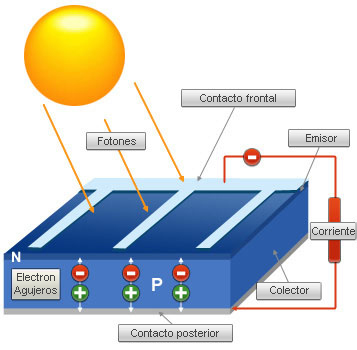
\includegraphics[scale=.50]{Capitulo2/images/celula-fotovoltaica.jpg}
	\caption{Efecto Fotoeléctrico}
	\label{fig:Efecto Fotoelectrico}
\end{figure}

\paragraph{}
Los paneles fotovoltaicos se clasifican en función del tipo de célula que los forman, hay células cristalinas y amorfas, las células cristalinas se dividen de la siguiente forma :

\begin{itemize}
	\item Monocristalinas: se componen de secciones de un único cristal de silicio reconocibles por su forma circular u octogonal.
	\item Policristalinas: cuando están formadas por pequeñas partículas cristalizadas.
\end{itemize}

\begin{figure}[H]
	\centering
	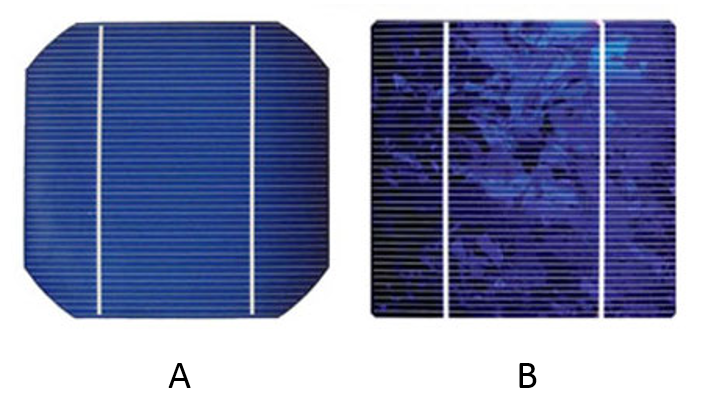
\includegraphics[scale=.50]{Capitulo2/images/tipospaneles.png}
	\caption{A: célula monocristalina ; B: célula policristalina}
	\label{fig:diagrama_dispensador}
\end{figure}

El costo de los paneles fotovoltaicos se ha reducido de forma constante desde que se fabricaron las primeras células solares comerciales y su costo promedio de generación eléctrica ya es competitivo con las fuentes de energía convencionales en un creciente número de regiones geográficas.
Los paneles fotovoltaicos pueden generar una gran cantidad de energía ya que en un día soleado, el Sol puede irradiar alrededor de 1kw por metro cuadrado a la superficie de la tierra, que sumado a la eficacia de estos paneles puede generar entre 120 y 250 w de manera constante por metro cuadrado, siempre dependiendo del tipo de panel y de su nivel de eficiencia.

\paragraph{Módulo Fotovoltaico 200W Policristalino IUSA}
Módulo fotovoltaico al estándar de las normas mexicanas NMX-J-643 y NMX-J-618, se muestra en la siguiente imagen, con 60 celdas en silicio policristalino, vidrio templado anti reflejante de 3.2 mm, caja de conexión IP67 con 3 diodos bypass y conectores compatibles con MC4.
Tiene una potencia máxima de 200W y un voltaje máximo de 30.6V, con una eficiencia del 15.1\% y temperatura de operación entre los -40ºC a los 85ºC. \citep{MarcoTeorico3}.

\begin{figure}[H]
	\centering
	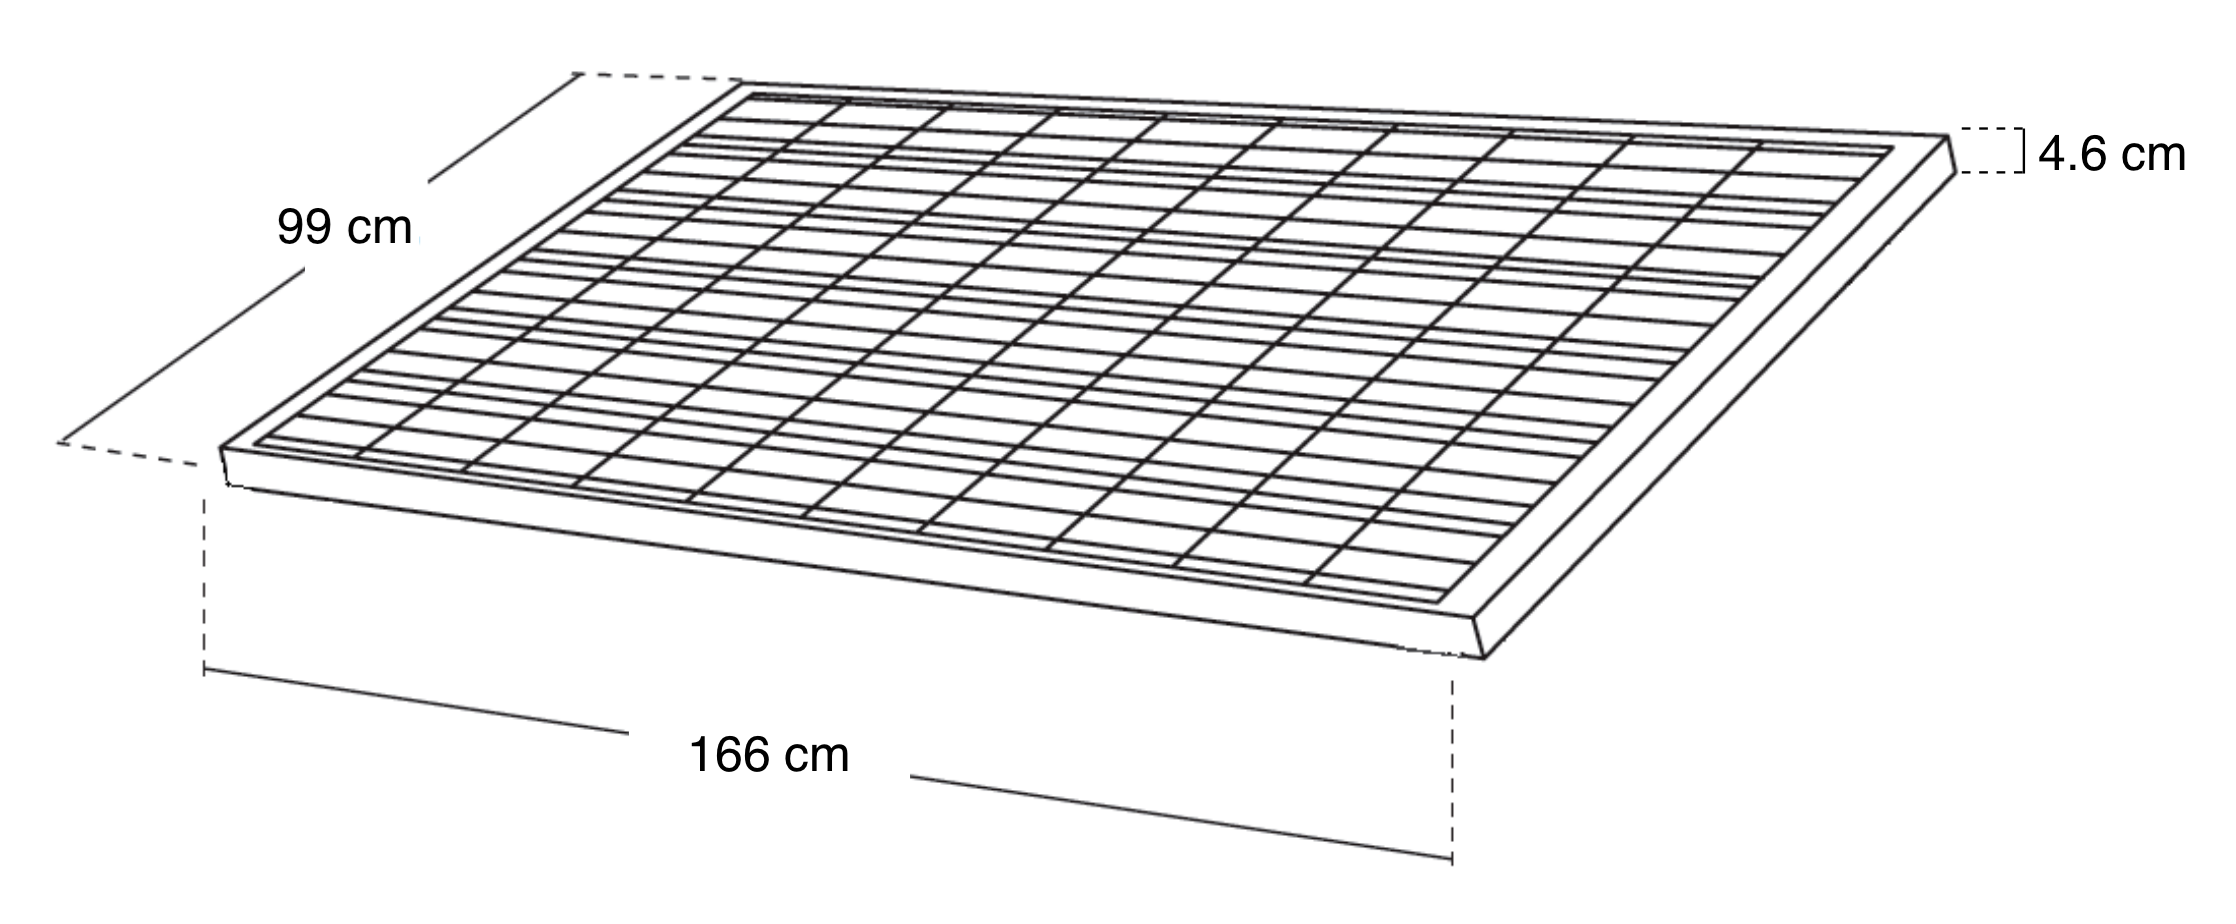
\includegraphics[scale=.25]{Capitulo2/images/panel.png}
	\caption{Módulo Fotovoltaico 250W Policristalino IUSA}
	\label{fig:diagrama_dispensador}
\end{figure}

\paragraph{Microinversor de corriente CC/CA para módulo fotovoltaico M1-01-250}
Diseñado específicamente para interconexiones en el sistema de distribución mexicano, con una salida de 127 V a 60 Hz CA y conector MC4 para conectar el panel solar \citep{MarcoTeorico3}.

\begin{figure}[H]
	\centering
	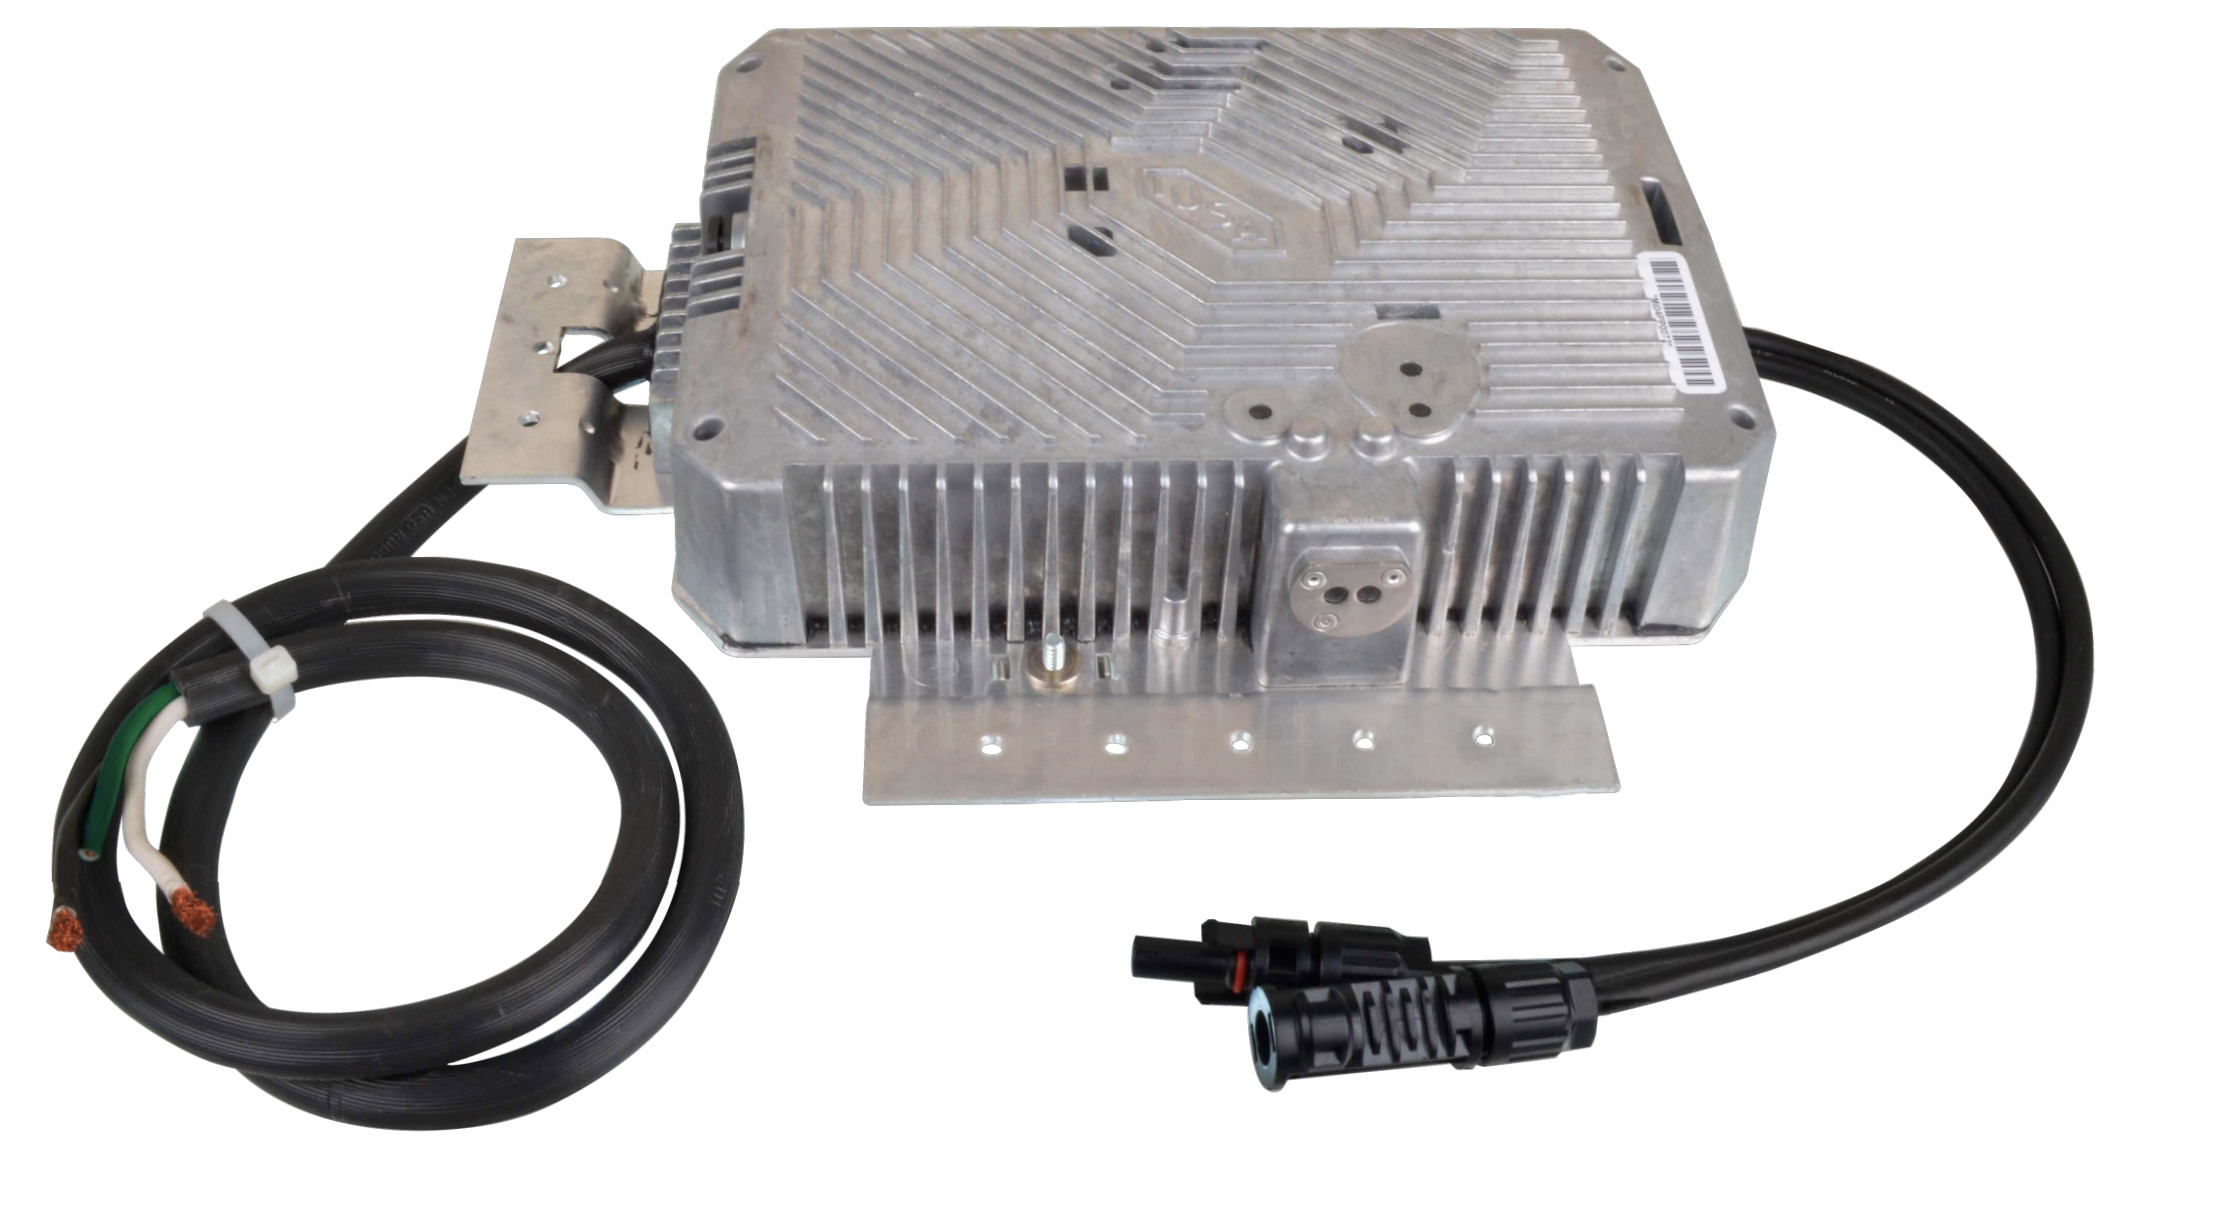
\includegraphics[scale=.20]{Capitulo2/images/microinversor.png}
	\caption{Microinversor M1-01-250}
	\label{fig:diagrama_dispensador}
\end{figure}


\paragraph{Factor de Potencia}
Para entender qué es el factor de potencia, primeramente vamos a definir una serie de conceptos básicos \citep{FP}.

kW.- Potencia de trabajo, también llamada potencia activa, potencia real, etc. Es la potencia que se transforma en trabajo útil.

kVAr.- Potencia reactiva. Es la potencia que los inductores necesitan para generar el flujo magnético y permitir crear un campo eléctrico.

kVA.- Potencia aparente. Es la suma vectorial de los kVAr más los kW.
 
El factor de potencia se define como la relación entre la potencia activa y la potencia aparente:

\[ FP = kW / kVAr + kVA \]

Esto quiere decir que, entre más potencia reactiva, menor factor de potencia, por lo tanto nuestro trabajo útil disminuirá y viceversa.\\

La relación entre estos tres conceptos se materializa en el triángulo de potencias:

\begin{figure}[H]
	\centering
	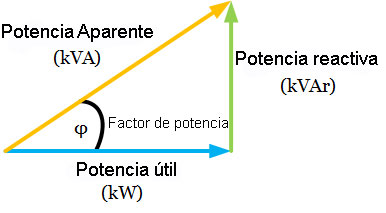
\includegraphics[scale=.50]{Capitulo2/images/triangulo-potencias.jpg}
	\caption{Triangulo de Potencias}
	\label{fig:diagrama_dispensador}
\end{figure}

\[ FP = kW / kVA = cos\theta \]
\[ FP = kVar / kVA = sin\theta \]


Por último, en este tema también es importante hablar de los tipos de cargas que existen:
\\
Resistencias.- Las resistencias se comportan como elementos no inerciales bajo el punto de vista de la relación tensión/intensidad, es decir, no se establece ninguna descoordinación temporal entre una y otra.\\

Inductancias.- Las inductancias, por el contrario, se comportan como elementos con una inercia no despreciable desde el punto de vista de la relación tensión/intensidad, provocando una descoordinación temporal, un retraso en este caso, de la intensidad en relación a la tensión de alimentación.\\

Capacitancias.- Finalmente las capacitancias, que se comportan también como elementos inerciales de naturaleza contraria a las inductancias, produciendo en este caso un adelanto de la intensidad en relación a la tensión de alimentación.
 
 \section{Wi-Fi}
 \paragraph{}
 Según la Real Academia Española es un sistema de conexión inalámbrica, dentro de un área determinada, entre dispositivos electrónicos, y frecuentemente para acceso a internet. En un sentido literal Wi-Fi no significa nada, es una marca comercial que también es usada para designar a las tecnologías de red sin cable.
 \paragraph{}
 En la actualidad es la que ofrece la mayor cantidad de beneficios al costo más bajo entre todas las tecnologías inalámbricas. Es económica, interoperable con equipos de diferentes fabricantes y puede ser extendida para ofrecer funcionalidades mucho más allá de las previstas originalmente por los fabricantes.
 
 \paragraph{Estándares 802.11}Los estándares inalámbricos son la base de muchos productos inalámbricos, lo que asegura su interoperabilidad y su usabilidad por parte de los que desarrollan, instalan y gestionan redes inalámbricas. Los estándares usados en la mayoría de las redes fueron establecidos por los grupos de trabajo 802 del IEEE. Los equipos de la familia de estándares 802.11 son, con mucho, los más fabricados e instalados para enlaces inalámbricos tanto de interiores como de exteriores. Las interfaces inalámbricas deben concordar en un canal común. Si un dispositivo está sintonizado en el canal 2, mientras que otra lo está en el canal 11, los radios no se podrán comunicar; de esto es lo que se encarga la familia de estándares 802.11 \citep{MarcoTeoricoWifi}.
\paragraph{}
Las redes Wi-Fi poseen una serie de ventajas, entre las cuales podemos destacar:
\begin{itemize}
	\item Al ser redes inalámbricas, la comodidad que ofrecen es muy superior a las redes cableadas porque cualquiera que tenga acceso a la red puede conectarse desde distintos puntos dentro de un espacio lo bastante amplio.
    \item Una vez configuradas, las redes Wi-Fi permiten el acceso de múltiples dispositivos sin ningún problema ni gasto en infraestructura, ni gran cantidad de cables.
    \item Asegura que la compatibilidad entre dispositivos es total, con lo que en cualquier parte del mundo podremos utilizar la tecnología Wi-Fi con una compatibilidad absoluta. 
\end{itemize}
 
 
 
\section{Módulo Wi-Fi MIKROE-2542}

MIKROE-2542 es una placa con un adaptador tipo mikroBUS que integra el módulo ESP-WROOM-02, este último está compuesto por una antena PCB y el chip ESP8266EX \citep{MarcoTeorico5}.

\begin{figure}[H]
	\centering
	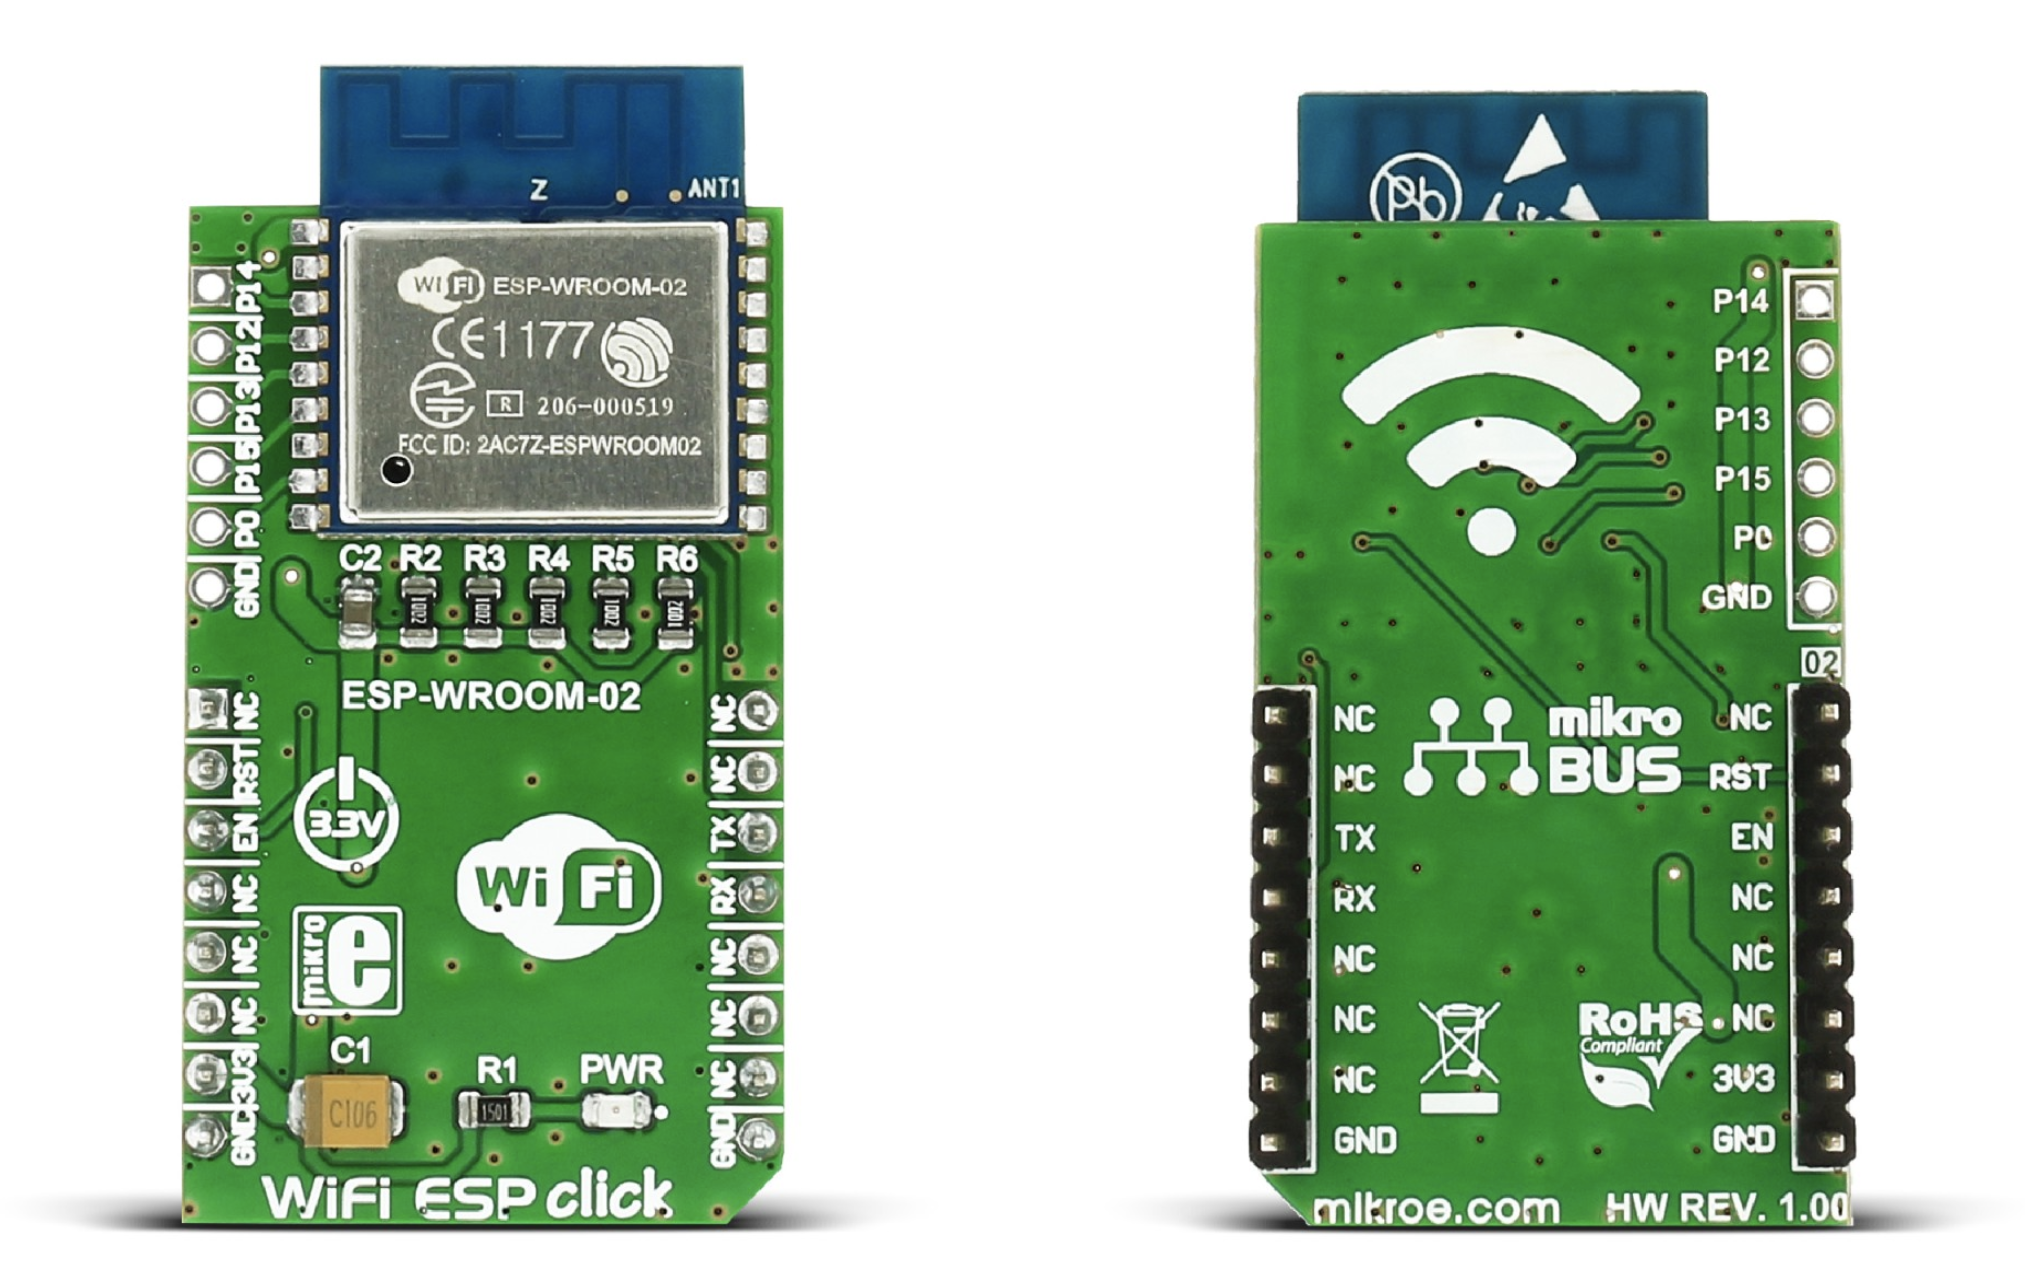
\includegraphics[scale=.4]{Capitulo2/images/mikroe.png}
	\caption{Placa MIKROE-2542, A:frontal; B:posterior}
	\label{fig:diagrama_dispensador}
\end{figure}
\paragraph{}

\begin{figure}[H]
	\centering
	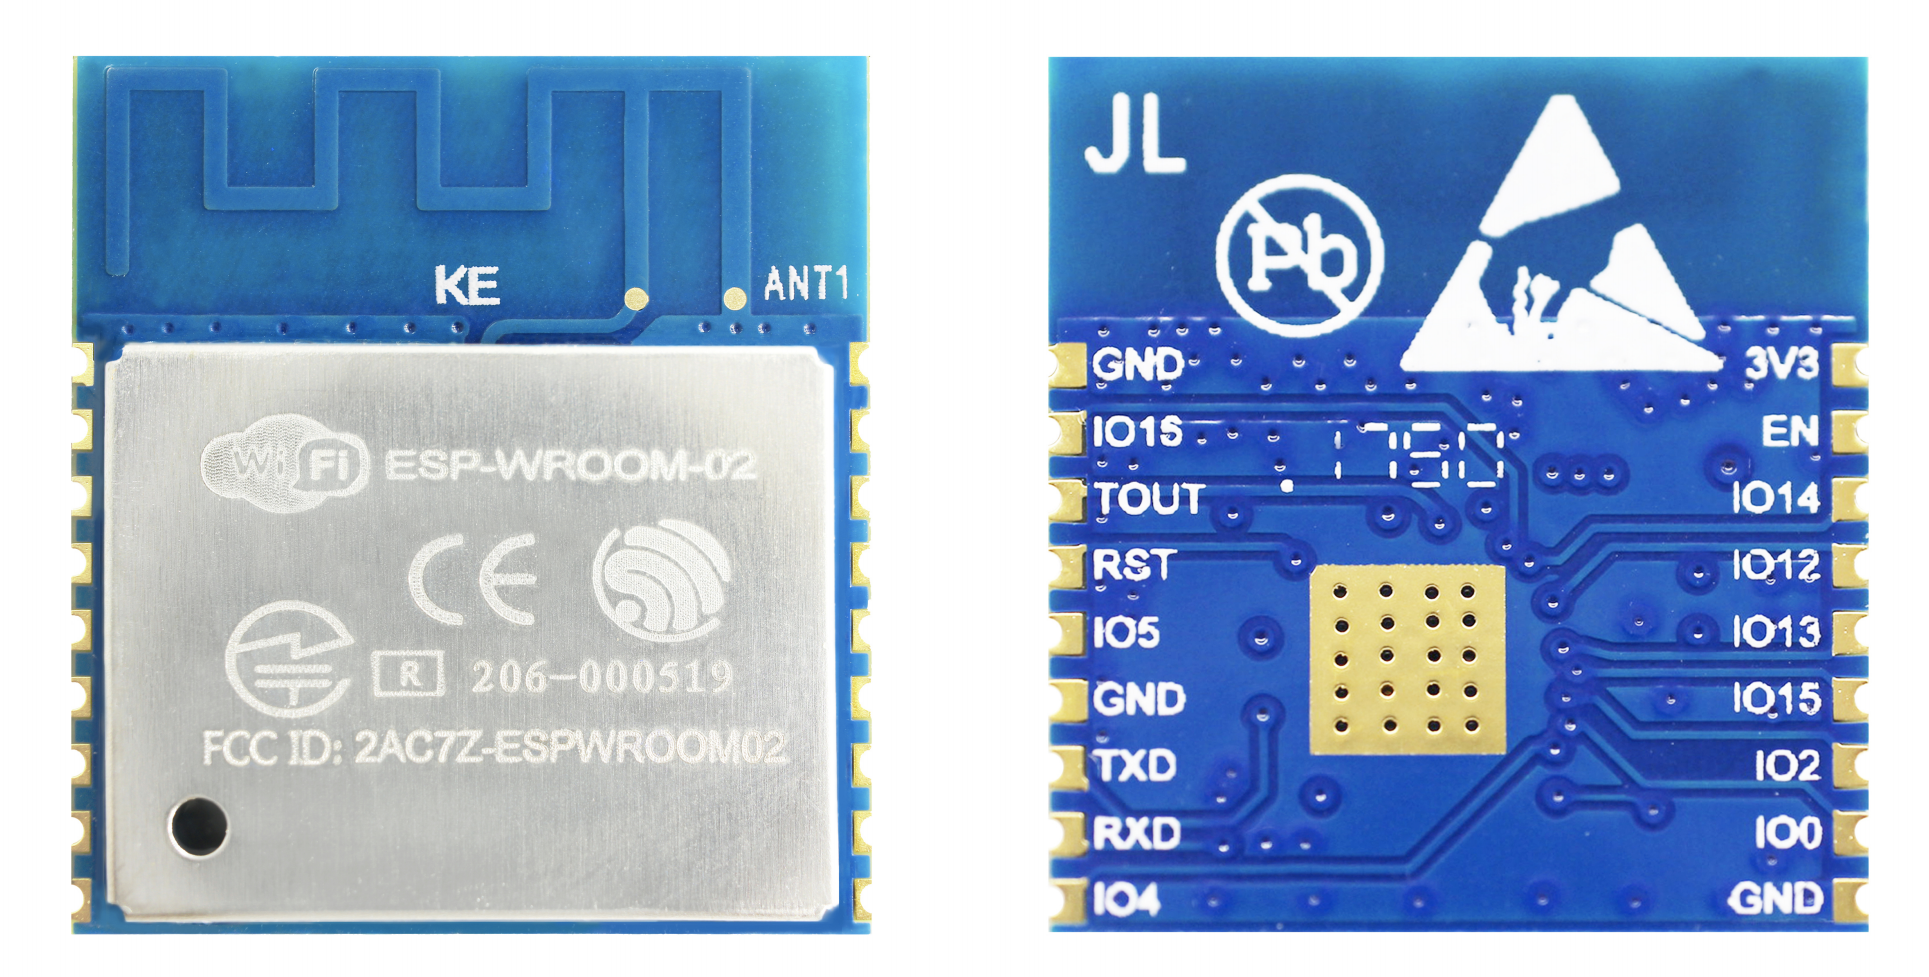
\includegraphics[scale=.2]{Capitulo2/images/wroom.png}
	\caption{Módulo ESP-WROOM-02, A:frontal; B:posterior}
	\label{fig:diagrama_dispensador}
\end{figure}


\paragraph{MikroBUS}
Es un estándar de distribución de los pines para la conexión y comunicación entre un microcontrolador o microprocesador con circuitos integrados o módulos, permitiendo así extender las capacidades de los mismos, este estándar incluye los pines requeridos por las tarjetas de desarrollo más actuales \citep{MarcoTeorico5}.
\begin{figure}[H]
	\centering
	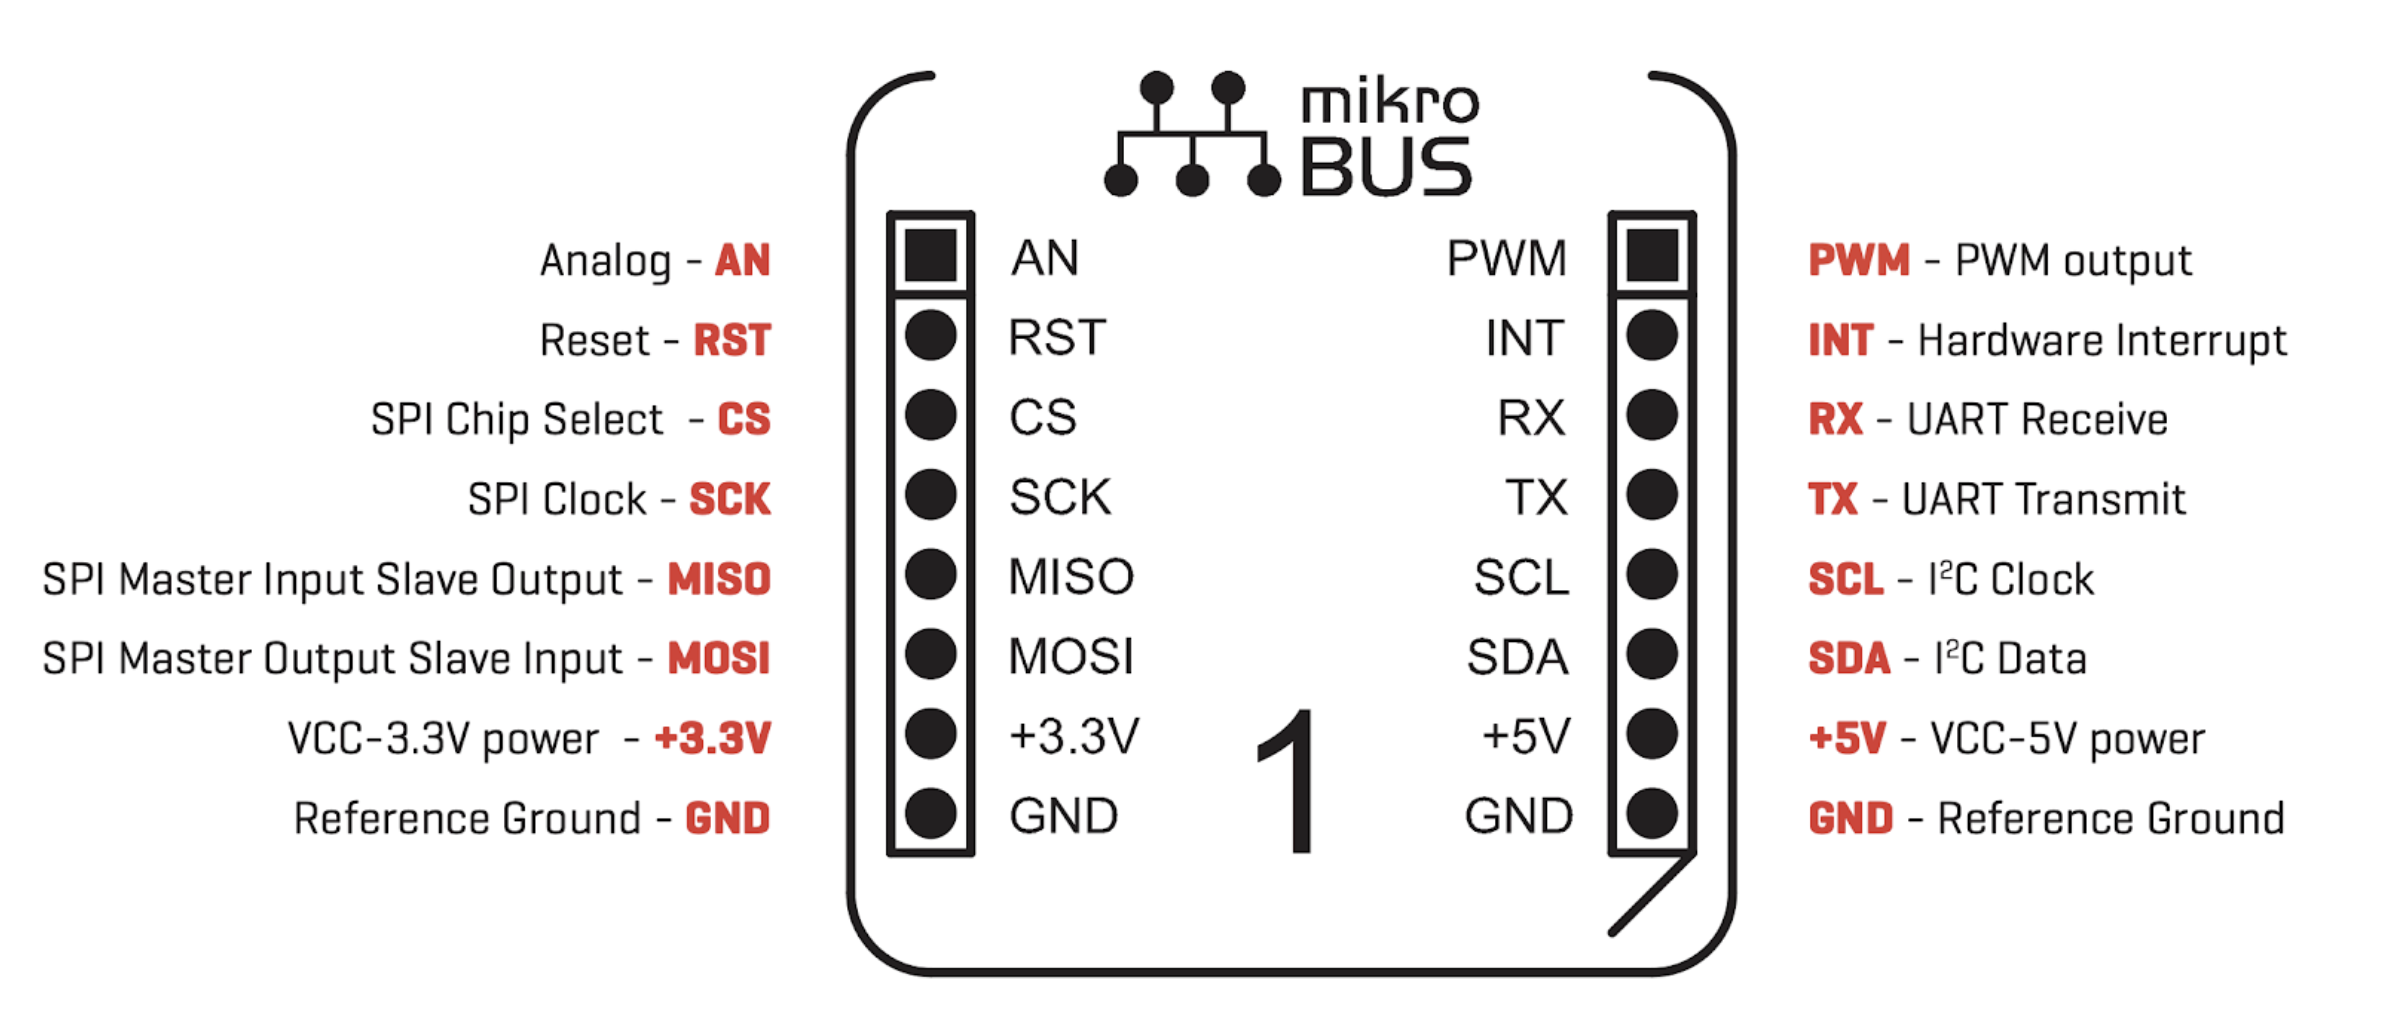
\includegraphics[scale=.25]{Capitulo2/images/mikrobus.png}
	\caption{Distribución de pines tipo MikroBUS}
	\label{fig:diagrama_dispensador}
\end{figure}
\paragraph{}

\paragraph{ESP8266}
El ESP8266 es un SoC Wi-Fi \citep{MarcoTeorico7} (System on Chip: integra todos o gran parte de los módulos que componen un sistema electrónico en un único circuito integrado) compuesto por una pila TCP/IP y un microcontrolador \citep{MarcoTeorico8}.
\paragraph{}

Este módulo permite a otros microcontroladores conectarse a un red inalámbrica Wi-Fi y realizar conexiones simples con TCP/IP haciendo uso eficiente de energía, lo cual lo hace ideal para proyectos de IoT. A continuación, se muestra una comparativa con otros módulos WiFi, la elección de este módulo es debido a que tiene solamente las características de comunicación WiFi necesarias y suficientes para la aplicación a desarrollar.

\begin{figure}[H]
	\centering
	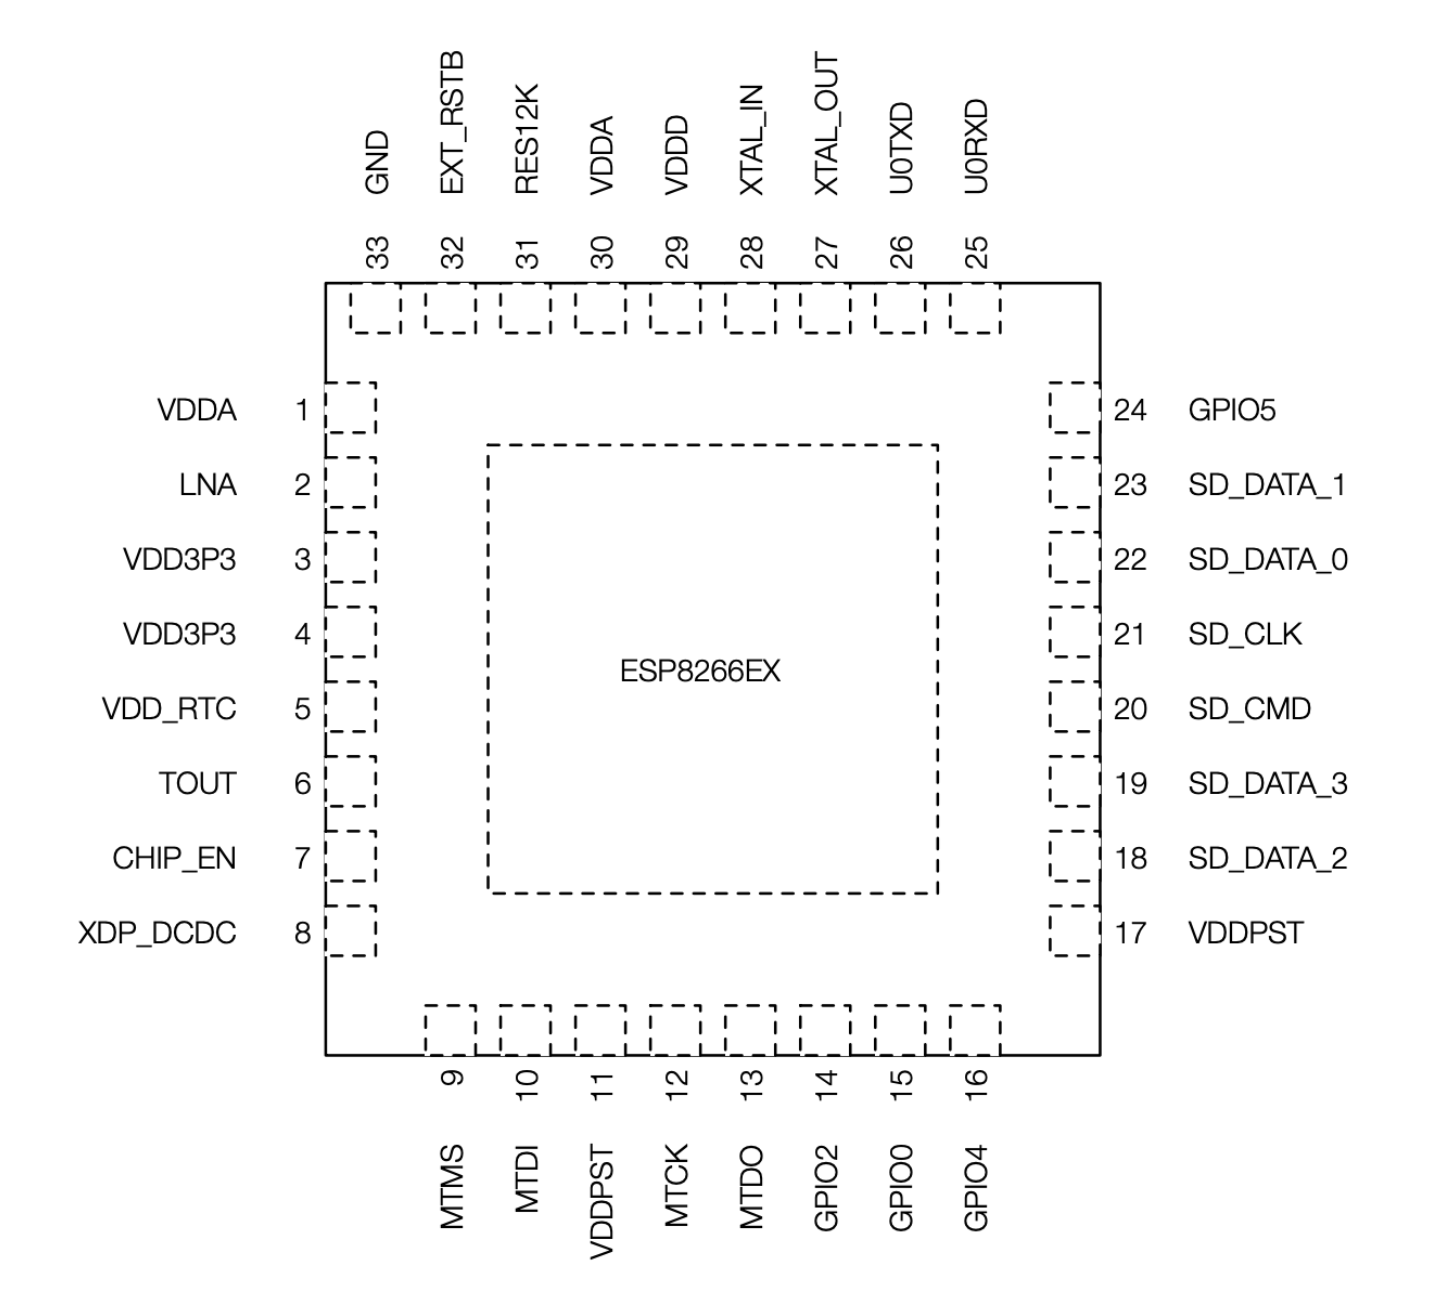
\includegraphics[scale=.3]{Capitulo2/images/esp8266.png}
	\caption{Diagrama esquemático del chip ESP8266}
	\label{fig:diagrama_dispensador}
\end{figure}

\pagebreak

\begin{longtable}{|M{2.2cm}|M{4.0cm}|M{4.0cm}|M{4.0cm}|}
    \caption{Comparativa módulos WiFi}
    \label{tabla_modulosWiFi}
	%\centering
	%\begin{tabular}
	\hline
	\textbf{Categoría} & \textbf{MIKROE-2542} & \textbf{356-ESP32-PICO-KIT} & \textbf{GPy 1.0} \\ \hline
	
 	Fabricante & MikroElektronika & Espressif Systems & Pycom
 	\hline
 	 
    Wi-Fi 
    &
    \newline  -Protocolo estándar IEEE 802.11
    \newline  -Rango de frecuencia 2.4G ~ 2.5G 
    \newline  -Antena PCB
	& 
    \newline  -Protoloco estándar IEEE 802.11
    \newline  -Rango de frecuencia 2.4G ~ 2.5G 
    \newline  -Antena 3D
	&   	    
    \newline  -Protoloco estándar IEEE 802.11
    \newline  -Rango de frecuencia 2.4G ~ 2.5G 
    \newline  -Antena Bluetooth y WiFi interna
    \newline  -Conector para antena LTE CAT M1 / NB1
    \newline  -Transceiver LTE CAT M1/ NB1 	
    \hline

	Bluetooth 
    &
	---
    &
	\newline Protocolo Bluetooth V4.2
	&
	\newline Protocolo Bluetooth V4.2 
	\hline
	
	Hardware &
    \newline  -CPU Tensilica L106 32-bit processor
    \newline  -Interfaz Periférica UART/SDIO/SPI/IIC/I2S/IR Control Remoto
    \newline  -Intefaces GPIO/ADC/PWM/LED Light
    \newline  -Voltaje de operación entre 2.5V ~ 3.6V
    &
    \newline  -CPU ESP32-PICO-D4
    \newline  -Interfaz Periférica ADC, DAC, sensor touch, SD/SDIO/MMC Host Controller, SPI, SDIO/SPI Controlador Esclavo, EMAC, motor PWM, LED PWM, UART, IIC, I2S, Control Remoto Infrarojo 
    \newline  -Voltaje de operación entre 2.5V ~ 3.6V
    \newline  -Sensor Hall integrado
    \newline  -Cristal de 40 MHz
    \newline  -SPI flash de 4MB integrada
    &
    \newline  - CPU Espressif ESP32 SoC
    \newline  - Coprocesador ULP
    \newline  - Interfaz Periférica ADC Controller
    \newline  - Voltaje de operación entre 2.5V ~ 3.6V
    \newline  - Memoria flash de 8MB integrada
    &
	\hline
	
    Precio (USD) & \$ 19.50 & \$ 13.00 & \$ 71.40
    \hline
	
	% \end{tabular}
	%\label{tabla_riesgos}
\end{longtable}

\pagebreak

\paragraph{}

\section{IoT (Internet de las cosas)}
De acuerdo con la definición otorgada por la IEEE, el internet de las cosas o IoT, es un dominio de aplicación que integra diferentes tecnologías y campos sociales, a pesar de la diversidad de las investigaciones sobre IoT \citep{MarcoTeoricoIoT}. El Internet de las cosas (IoT) se está convirtiendo en un tema de conversación cada vez más creciente tanto en el lugar de trabajo como fuera de él. Es un concepto que no sólo tiene el potencial de impactar cómo vivimos, sino también cómo trabajamos. 
\paragraph{}
El Internet de banda ancha está cada vez más disponible, el costo de la conexión reduciendo, se están creando más dispositivos con capacidades Wi-Fi y sensores integrados, los costos de la tecnología están disminuyendo y la penetración de los teléfonos inteligentes disparando. En pocas palabras, este es el concepto de conectar básicamente cualquier dispositivo con un interruptor de encendido y apagado a Internet. Esto incluye todo, desde teléfonos celulares, cafeteras, lavadoras, audífonos, lámparas, dispositivos portátiles y casi cualquier otra cosa que se pueda imaginar. Esto también se aplica a los componentes de las máquinas. La firma de analistas Gartner dice que para 2020 habrá más de 26 mil millones de dispositivos conectados. El IoT es una red gigante de cosas conectadas (que también incluye a las personas). La relación será entre personas-personas, personas-cosas y cosas-cosas.
\paragraph{}
Hay muchos ejemplos de cómo podría verse esto o cuál podría ser el valor potencial. Digamos, por ejemplo si se está en camino a una reunión; el automóvil podría tener acceso a su calendario y ya sabe cuál es la mejor ruta a seguir. Si el tráfico es intenso, el automóvil podría enviar un mensaje de texto a la otra parte notificándole que llegará tarde. 
\paragraph{}
La realidad es que el IoT permite oportunidades y conexiones virtualmente infinitas, muchas de las cuales ni siquiera podemos pensar o entender completamente su impacto. Ciertamente abre la puerta a muchas oportunidades pero también a muchos desafíos. La seguridad es un gran problema que a menudo se plantea. Luego tenemos el tema de la privacidad y el intercambio de datos. Este es un tema candente incluso hoy en día, por lo que sólo se puede imaginar cómo la conversación y las preocupaciones aumentarán cuando se habla de la conexión de muchos miles de millones de dispositivos \citep{MarcoTeoricoIoT2}. 



\section{Demonio / Servicio}
Un demonio o servicio es un programa que se ejecuta en segundo plano, fuera del control interactivo de los usuarios del sistema, ya que carecen de interfaz con estos. El término demonio se usa fundamentalmente en sistemas UNIX y basados en UNIX, como GNU/Linux o Mac OS X \citep{MarcoTeorico4}.


\section{Ubuntu Core}

El sistema Operativo Ubuntu es largamente distribuido a través de distintos sectores privados y públicos por millones de personas y organizaciones por su fiabilidad y tiempo en el campo de servidores de información.

Ubuntu Core es un sistema operativo basado en UNIX enfocado para dispositivos IoT, siendo una versión mínima y de gran rendimiento de Ubuntu, altamente segura con actualizaciones aseguradas por los próximos 10 años.
\paragraph{}
Ubuntu Core tiene como características mayor rapidez, confiabilidad por medio de uso de actualizaciones transaccionales, lo cual significa que cada acción se realiza con éxito o no se realiza, teniendo la posibilidad de hacer un rollback si es necesario, características que una distribución de Linux tradicional no ofrece.
\paragraph{}
La tabla \ref{UbuntuCore} nos muestra una comparativa que permite ver que, gracias a su necesidad de poco uso de procesamiento y almacenamiento, es indicado para usasr como servidor embebido.
\paragraph{}
\begin{longtable}{|M{3.2cm}|M{4.0cm}|M{4.0cm}|M{4.0cm}|}
    \caption{Comparativa del sistema operativo Ubuntu Core con su versión clásica}
    \label{UbuntuCore}
	%\centering
	%\begin{tabular}
	\hline
	\textbf{Característica} & \textbf{Ubuntu Core} & \textbf{Ubuntu Clásico} \\ \hline
 	 
    Requerimientos Mínimos
    
    &
    
    \newline  -500 MHz single core processor
    \newline  -256 MB RAM
    \newline  -512 MB storage

	&
	
    \newline  -1 GHz dual core processor
    \newline  -512 MB RAM
    \newline  -1.5 GB storage
    \hline
        
	Interfaz Gráfica
    &
	\newline Ninguna por default pero pueden descargarse en caso de ser necesario
    &
	\newline Xorg y GNOME Shell o Wayland y GNOME Shell
	\hline
	
	
	% \end{tabular}
	%\label{tabla_riesgos}
\end{longtable}


\section{Red de sensores}
Una red de sensores consiste en un conjunto de dispositivos denominados sensores que están conectados entre sí, para el monitoreo y sensado de condiciones físicas y/o ambientales en áreas remotas; dichos sensores pueden estar distribuidos físicamente y para referirnos a un sensor en específico como parte de la red, se le denomina nodo sensor. 
\paragraph{}
El propósito de una red de sensores es el de recolectar información de interés, es decir, la variable física sensada o monitoreada, para posteriormente transmitir dicha información con el objeto de ser procesada y analizada. 
\paragraph{}
Dado que existen una gran cantidad de dispositivos sensores implica que pueden implementarse diferentes tipos de redes de sensores de acuerdo al uso o aplicación que se le quiera dar, como por ejemplo: fenómenos meteorológicos, sistemas de emergencia o de cuidados médicos, por mencionar algunos \citep{MarcoTeorico16}.

\paragraph{Sensor}
Un sensor es un dispositivo que es capaz de transformar una señal o variable proveniente de fenómenos físicos, como pueden ser: temperatura, presión, humedad, aceleración, entre otros; en una señal de salida transducible a una señal eléctrica \citep{MarcoTeorico20} .
\paragraph{}
Existe una variedad de sensores, y pueden ser clasificados bajo diferentes criterios (principio de funcionamiento, señal de salida, rango de valores, nivel de integración, variable física de entrada).

\paragraph{MCP39F521}
Este sensor, el cual se define como un dispositivo de alta integración de monitoreo de energía de fase completa, diseñado para realizar medición en tiempo real de la energía de entrada para las fuentes de alimentación de corriente directa o alterna, unidades de distribución de energía y aplicaciones de consumidor e industriales. Una de las características de este dispositivo que importa señalar, es que cuenta con una interfaz IIC, como se puede observar en la figura \ref{fig:Diagrama a bloques del MCP39F521}, dicha interfaz tiene una velocidad de reloj de hasta 400 kHz \citep{MarcoTeorico13}; de esta forma es como se realizará la comunicación que permita el intercambio de la información monitoreada con el microcontrolador. 
\paragraph{}
\begin{figure}[H]
	\centering
	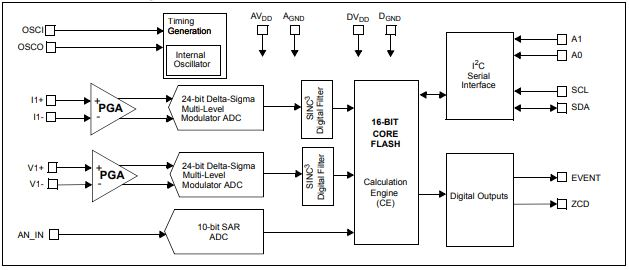
\includegraphics[scale=.9]{Capitulo2/images/DiagramaDispMonitoreo.JPG}
	\caption{Diagrama a bloques del MCP39F521}
	\label{fig:Diagrama a bloques del MCP39F521}
\end{figure}

\begin{longtable}{|M{2.2cm}|M{4.0cm}|M{4.0cm}|M{4.0cm}|}
    \caption{Comparativa de Monitores de Potencia y Corriente}
    \label{tabla_modulosWiFi}
	%\centering
	%\begin{tabular}
	\hline
	\textbf{Categoría} & \textbf{MCP39F521} & \textbf{ISL28025} \\ \hline
	
 	Fabricante & Microchip & Renesas Electronics
 	\hline
 	 
    Protocolo de Comunicación 
    &
    \newline  I2C
	& 
    \newline  I2C
    \hline

	Características

    &
	\newline -Monitoreo de potencia activa, potencia reactiva, potencia aparente, voltaje RMS, corriente RMS, factor de potencia y linea de frecuencia. 
	\newline -Precisión del 99.99\%
	\newline -Rutina de calibración rápida y comandos simplificados
	\newline -Detector de cruce en cero

	&
	\newline -Monitoreo de voltaje, corriente y potencia 
	\newline -Precisión del 99.99\%
	\newline -Sensado de corriente bidireccional
	\hline
	
	Precio (USD) 
	
	&
	\newline \$ 3.37
	&
	\newline \$ 5.59
	\hline

\end{longtable}


\paragraph{IIC}
IIC es una interfaz serial síncrona de comunicación, la cual es útil para comunicarse  con otros periféricos y microcontroladores, fue desarrollada por Philips Semiconductors.
Estos periféricos pueden ser: Memorias seriales EEPROMS, registros de corrimiento, expansores de puerto, ADC's, DAC's, entre otros \citep{MarcoTeorico17}.
\paragraph{}
Sólo se utilizan dos líneas para comunicación:
\begin{itemize}
	\item Una línea de datos serial (SDA)
    \item Una línea de reloj serial (SCL), que siempre es generada por el maestro.
\end{itemize}

Cada dispositivo conectado al bus es reconocido por una única dirección, el bus maneja una arquitectura maestro-esclavo, el maestro trabaja como transmisor o receptor, donde el maestro inicia y termina la transferencia de información.

\begin{figure}[H]
	\centering
	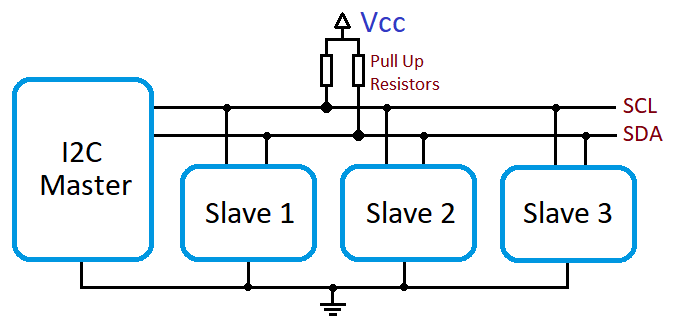
\includegraphics[scale=.35]{Capitulo2/images/I2C-Interface.png}
	\caption{Diagrama ejemplificativo de interfaz IIC}
	\label{fig:}
\end{figure}

Entre las características principales están:
\begin{itemize}
	\item Se realizan transferencias seriales bidireccionales de 8 bits.
    \item Se proporciona filtrado en Chip para eliminar picos en la línea de datos y preservar integridad de datos.
    \item El número de circuitos integrados que pueden ser conectados al bus está limitado a la capacitancia máxima del bus.
    \item Modo estándar de operación (Standard Mode). Con velocidad de hasta 100 kbps.
    \item Modo rápido de operación  (Fast mode). Con velocidad de hasta 400 kbps. \item Modo más rápido de operación (Fast mode plus). Con velocidad de hasta 1 Mbps.
\end{itemize}

Para que la transferencia de información pueda ser iniciada, el bus debe estar libre. Todas las transacciones comienzan con START y pueden ser terminadas por un STOP.
Una transición de alto a bajo en la línea SDA mientras SCL es alto, define una condición de START.
Una transición de bajo a alto en la línea SDA mientras SCL es alto, define una condición de STOP.

\begin{figure}[H]
	\centering
	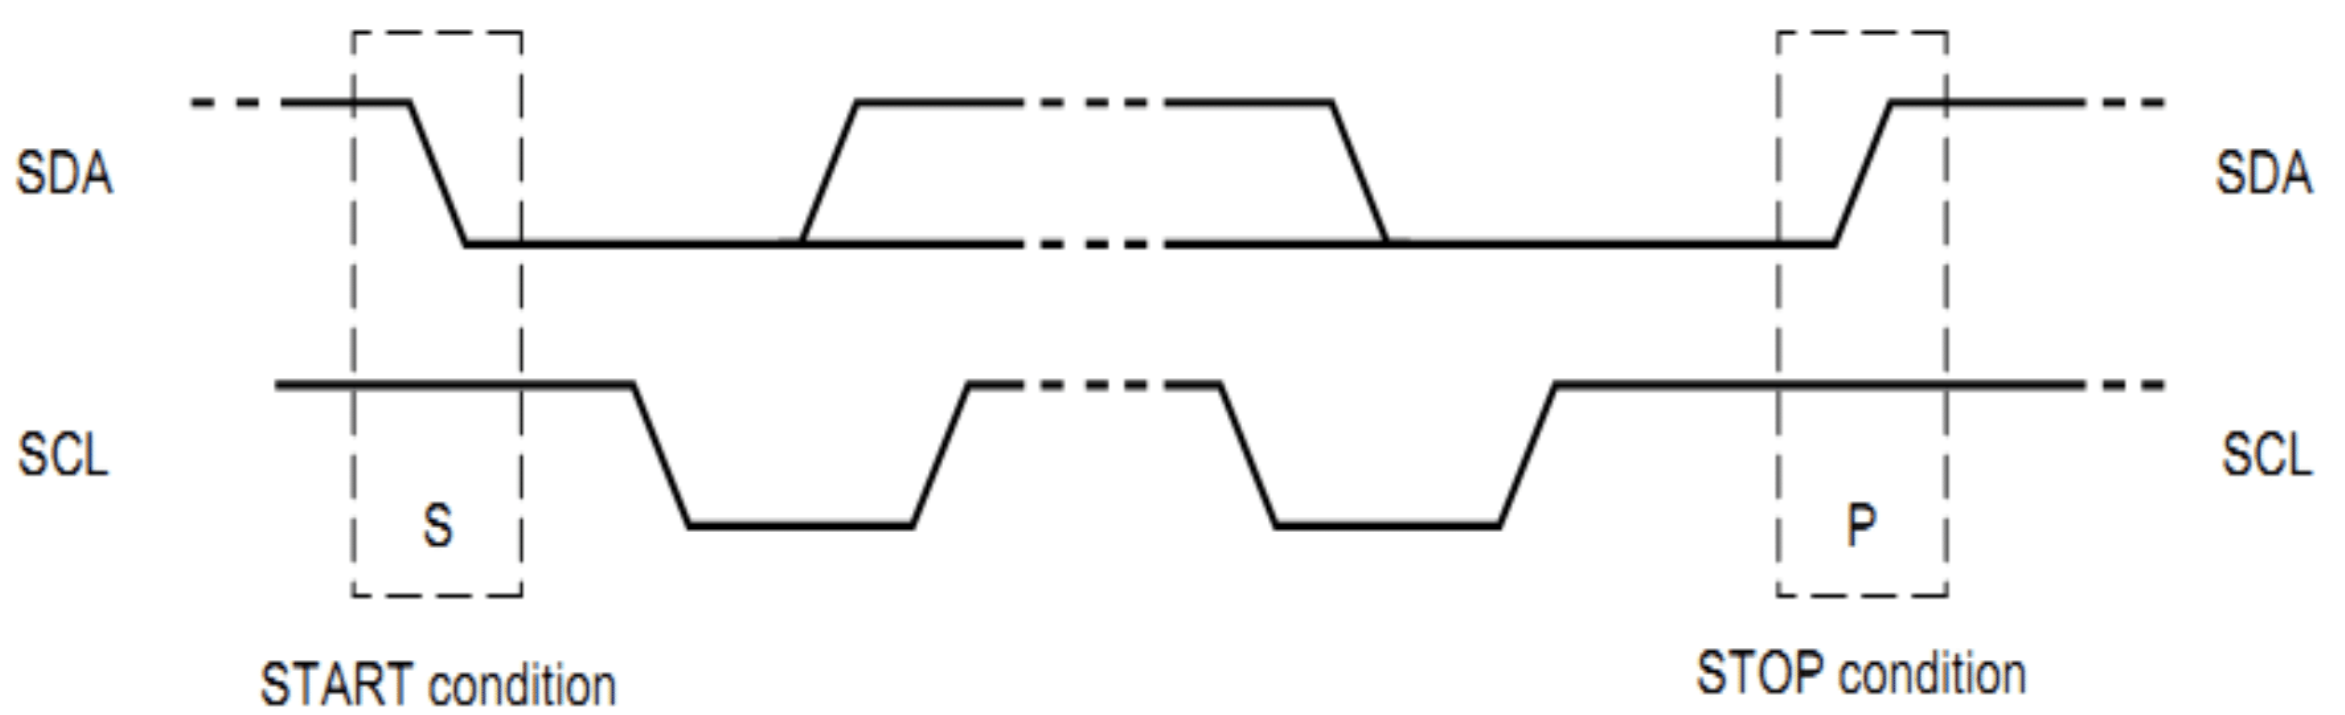
\includegraphics[scale=.25]{Capitulo2/images/startstop.png}
	\caption{Protocolo de START y STOP}
	\label{fig:}
\end{figure}




\section{Dispositivo de monitoreo de energía}
En este trabajo se plantea el uso de un dispositivo de monitoreo de energía que permita supervisar de manera constante la energía producida por un sistema fotovoltaico; es por ello que a continuación definiremos algunos conceptos importantes.
\paragraph{}
Inicialmente, un dispositivo puede ser definido como un mecanismo dispuesto para obtener un resultado automático \citep{MarcoTeorico11}; es decir, un conjunto de elementos bien definidos, que entre sí, realizan acciones conforme la información recibida (entrada) para poder transformarla (salida).
Existe una amplia gama de clasificación de dispositivos de acuerdo al propósito para el que es empleado, sin embargo, para fines de este trabajo, el dispositivo de interés entra en la categoría de aquellos que se encargan de monitorear. 
\paragraph{}
De acuerdo a la Real Academia Española, la palabra monitorear, se define como la acción de observar, supervisar o controlar mediante aparatos especiales, el curso de uno o varios parámetros fisiológicos o de otra naturaleza para detectar posibles anomalías \citep{MarcoTeorico12}.
\paragraph{}
Teniendo en cuenta los 2 conceptos anteriores, podemos definir a un dispositivo de monitoreo de energía como: un mecanismo que recibe como entrada energía e internamente procesa dicha información para finalmente arrojar datos de monitoreo.


\section{Sistema Embebido}
Un sistema embebido es un dispositivo diseñado para un propósito en específico, el cual abarca desde una operación hasta un conjunto pequeño de operaciones en tiempo real, a diferencia de una PC, la cual puede realizar una gran cantidad de tareas de acuerdo a los programas que se ejecuten. 
\paragraph{}
El uso de los sistemas embebidos ha cobrado gran importancia debido a los usos y aplicaciones que se le han dado, como son: hornos de microondas, máquinas expendedoras, routers, cámaras digitales, reproductores MP3, entre otros. 
\paragraph{}
Algunas de las características principales de los sistemas embebidos son: que tienden a ser de dimensiones pequeñas, son considerados económicos o de bajo costo, su nivel de consumo eléctrico es bajo, poseen recursos limitados de memoria así como de dispositivos de entrada/salida \citep{MarcoTeorico14}.
\paragraph{}
Por lo general, los sistemas embebidos al ofrecer como ventaja la realización de operaciones en tiempo real, suelen ser empleados en ambientes físicos donde se hace uso de sensores y actuadores. Se dice que son sistemas reactivos, pues están en interacción continua con su entorno y el ritmo de su ejecución está coordinada con dicho entorno. 
\paragraph{}
Los sistemas embebidos suelen tener en una de sus partes una computadora con características especiales conocida como microcontrolador que viene a ser el cerebro del sistema, el cual incluye interfaces de entrada/salida en el mismo chip. Normalmente estos sistemas poseen una interfaz externa para efectuar un monitoreo del estado y hacer un diagnóstico del sistema \citep{MarcoTeorico15}.
\paragraph{}
Los sistemas embebidos pueden ser implementados en placas únicas (SBC) y sobre estas se encuentran integrados los recursos de hardware como el microprocesador, la memoria RAM, controladores Ethernet, etc \citep{MarcoTeorico14}.
\paragraph{SBC}
SBC por sus siglas en inglés, Single Board Computer es, como su nombre lo indica, una Computadora de Placa Única, lo cual implica que tiene la totalidad o cumple con la mayoría de las características que tienen las computadoras personales pero en una placa de circuito; sin embargo al tratarse de una placa, es de menores dimensiones así como de un precio relativamente más bajo.
\paragraph{}
Dependiendo el tipo de SBC, pueden llegar a ejecutar como Sistema Operativo Linux, Android o Windows. También cuentan con puertos de Entrada/Salida de propósito general, los cuales permiten la comunicación con otros dispositivos \citep{MarcoTeorico18}. 
\paragraph{}
Algunos ejemplos de SBC son la Raspberry Pi, Banana Pi, BeagleBone Black, PcDuino, entre otros.
\paragraph{Raspberry Pi}
En este trabajo, haremos uso de la Raspberry Pi. Como se menciona en el párrafo anterior, es una SBC. Fue desarrollada en el Reino Unido por la fundación Raspberry Pi con el propósito de promover la educación informática en las escuelas. Algunas de sus principales características son: corre en el sistema operativo Linux así como en Raspbian y Pidora, las cuales son distribuciones de Linux; además tiene conexión a monitor, teclado y mouse \citep{MarcoTeorico19}.   

A continuación, se muestra una comparativa entre la Raspberry Pi 3B y la Banana Pi M2 Berry \citep{MarcoTeorico21}\citep{MarcoTeorico22}.

\begin{figure}[H]
	\centering
	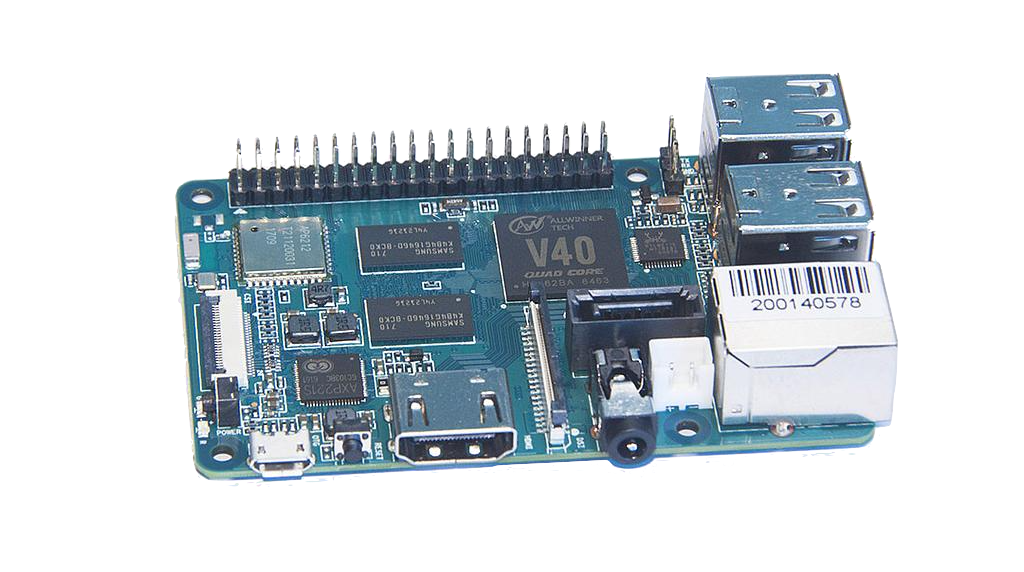
\includegraphics[scale=.3]{Capitulo2/images/bananaPi.png}
	\caption{Banana Pi M2 Berry}
	\label{fig:}
\end{figure}

\paragraph{}
\begin{figure}[H]
	\centering
	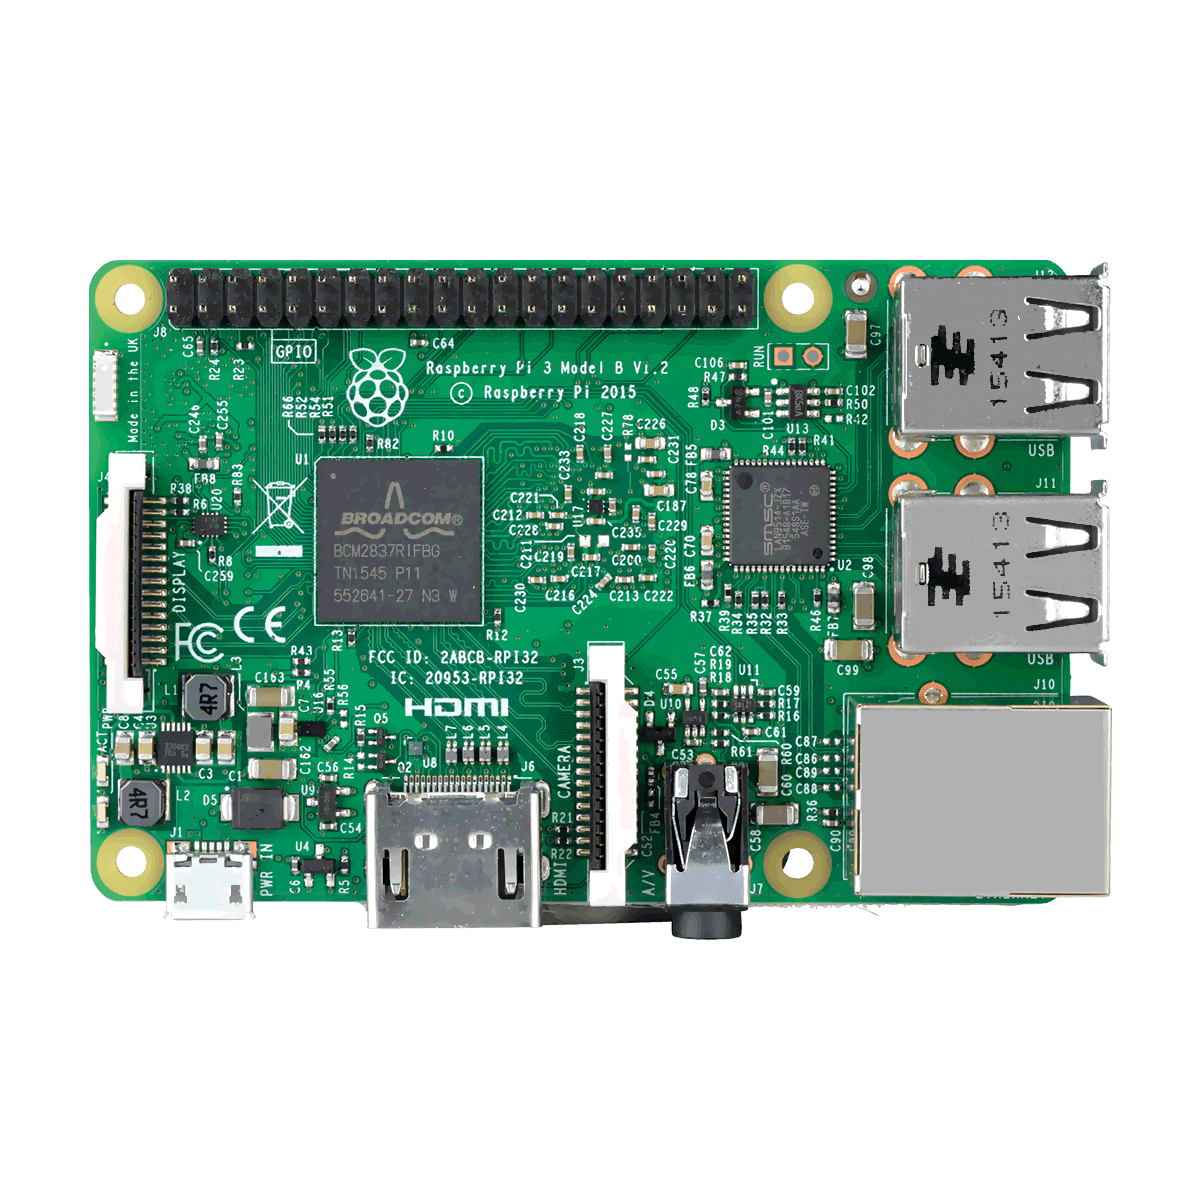
\includegraphics[scale=.23]{Capitulo2/images/raspberry.png}
	\caption{Raspberry Pi 3B}
	\label{fig:}
\end{figure}

\pagebreak
\begin{longtable}{|M{3.0cm}|M{4.5cm}|M{4.5cm}|}
    \caption{Comparativa entre Banana Pi M2 Berry y Raspberry Pi 3B}
%\begin{table}[!hbt]
	% \centering
	 %\begin{tabular}{|M{3.0cm}|M{4.5cm}|M{4.5cm}|}
	\hline
	\textbf{Característica} & \textbf{Banana Pi M2 Berry} & \textbf{Raspberry Pi 3B} \\ 
	\hline
 	Procesador & Quad Core ARM Cortex A7 V40 & Quad Core 64bit ARM Cortex A53 1.2GHz \\
 	\hline
    GPU & 500 MHz Mali-400 MP2 & 400 MHz VideoCore IV multimedia\\
    \hline
    RAM & 1GB DDR3 SDRAM & 1GB LPDDR2-900 SDRAM \\
	\hline
	Tarjeta de Red & 10/100/1000 Mbps Ethernet y 802.11 b/g/n & 10/100 Mbps Ethernet y 802.11n Wireless LAN\\
	\hline
	Almacenamiento & Micro SD (hasta 64 GB) & Micro SD\\
	\hline
	Salida Video & HDMI, MIPI DSI para paneles LCD & HDMI\\
    \hline
    Salida Audio 
    & 
    \newline - HDMI 
    \newline - Jack 3.5 mm 
    & 
    \newline - HDMI
    \newline - Jack 3.5 estéreo \\
    \hline
    USB & 
    \newline - 4x USB 2.0 
    \newline - USB OTG(Micro USB) 
    & 
    \newline - 4x USB 2.0
    \newline - 1x micro USB alimentación \\
    \hline
    Sistema Operativo 
    & 
    \newline - Raspbian
    \newline - NetBSD
    \newline - Android
    \newline - Debian 
    &
    \newline - Linux
    \newline - Raspbian
    \newline - Pidora \\
    \hline
    Precio & \$3,359 MX & \$900 MX \\
    %https://articulo.mercadolibre.com.mx/MLM-632513569-raspberry-pi-3-model-b-3b-_JM?quantity=1
    %https://articulo.mercadolibre.com.mx/MLM-648967037-quad-core-cortex-a7-cpu-1g-ddr-banana-pi-bpi-m2-berry-same-_JM?quantity=1
	\hline
	%\end{tabular}
	
	%\label{tabla_riesgos}
\end{longtable}



\section{Microcontroladores}
Hoy en día, los conteos de producción de microcontroladores son de miles de millones por año, y los controladores están integrados en muchos dispositivos a los que nos hemos acostumbrado, como electrodomésticos (microondas, lavadora, cafetera, etc.), telecomunicaciones (teléfonos móviles), industria automotriz (inyección de combustible, frenado ABS, etc.), industria aeroespacial, automatización industrial, entre otros.
\paragraph{}
Un Microcontrolador es un circuito integrado que es el componente principal de una aplicación embebida. Es como una pequeña computadora que incluye sistemas para controlar elementos de entrada/salida. También incluye a un procesador y por supuesto memoria que puede guardar el programa y sus variables (flash y RAM).  Funciona como una mini PC. Su función es la de automatizar procesos y procesar información.
El microcontrolador se aplica en toda clase de inventos y productos donde se requiere seguir un proceso automático dependiendo de las condiciones de distintas entradas.
\paragraph{}
Los diseños internos básicos de los microcontroladores son bastante similares. La figura \ref{fig:diagrama_micro} muestra el esquema de un microcontrolador típico. Todos los componentes están conectados a través de un bus interno y son todos integrados en un chip. Los módulos están conectados al mundo exterior a través de pines de E/S.
\paragraph{}
\begin{figure}[H]
	\centering
	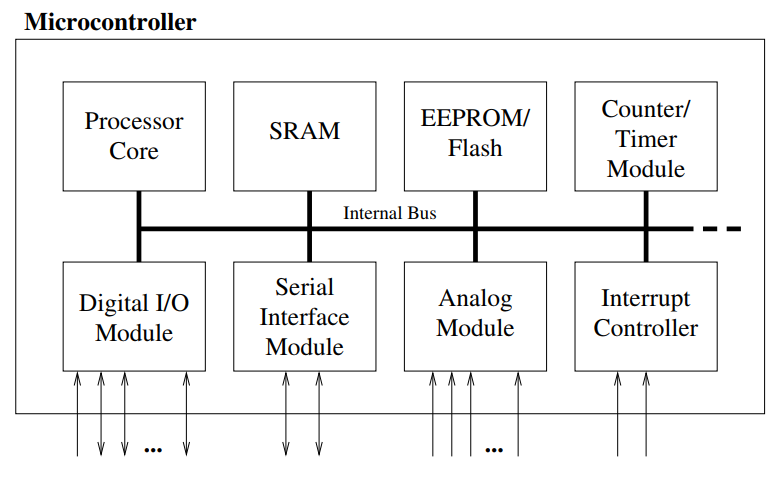
\includegraphics[scale=.5]{Capitulo2/images/microcontrolador.png}
	\caption{Diagrama de un microcontrolador básico}
	\label{fig:diagrama_micro}
\end{figure}
\paragraph{}
En la siguiente lista mostramos los módulos que normalmente se encuentran en un microcontrolador \citep{MarcoTeoricoMicrocontrolador}:
\begin{itemize}
	\item Procesador Core: La CPU del controlador. Contiene la unidad lógica aritmética, la unidad de control y los registros (puntero de pila, contador de programa, registro de acumulador, archivo de registro, ...).
    \item Memoria: La memoria a veces se divide en memoria de programa y memoria de datos. En los controladores más grandes, un controlador DMA maneja las transferencias de datos entre los componentes periféricos y la memoria.
    \item Controlador de interrupciones: Las interrupciones son útiles para interrumpir el flujo normal del programa en caso de (importantes) eventos externos o internos. En conjunción con los modos de sueño, ayudan a conservar energía.
    \item Temporizador o contador: La mayoría de los controladores tienen entre uno y tres temporizadores o contadores, que se pueden usar para marcar la hora de eventos, medir intervalos o contar eventos.
    \item E / S digital: Los puertos de E / S digitales paralelos son una de las características principales de los microcontroladores. La cantidad de pines de E / S varía de 3 a más de 90.
    \item E / S analógicas: Aparte de unos pocos controladores pequeños, la mayoría de los microcontroladores tienen integrado convertidores analógico - digital, que difieren en el número de canales (2-16). 
    \item Interfaces: Los controladores generalmente tienen al menos una interfaz en serie que se puede utilizar para descargar el programa y para la comunicación con la PC de desarrollo en general. Dado que las interfaces seriales también pueden usarse para comunicarse con dispositivos periféricos externos, la mayoría de los controladores ofrecen varias y variadas interfaces como SPI y SCI.
    \item Temporizador de vigilancia: Dado que los sistemas críticos para la seguridad forman un área importante de aplicación de los microcontroladores, es importante protegerse contra errores en el programa y / o el hardware. El temporizador de vigilancia se usa para reiniciar el controlador en caso de que el software se "bloquee".
    \item Unidad de depuración: Algunos controladores están equipados con hardware adicional para permitir la depuración remota del chip desde la PC. Así que no hay necesidad de descargar un software especial de depuración.
\end{itemize}

\paragraph{}
En la siguiente tabla, se muestra una comparativa entre los microcontroladores dsPIC30F3014/4013 y dsPIC30F1010/202X.


\pagebreak
\begin{longtable}{|M{2.2cm}|M{6.0cm}|M{6.0cm}|}
    \caption{Comparativa entre microcontroladores}
	% \centering
	% \begin{tabular}
	\hline
	\textbf{ Parámetro } & \textbf{Microcontrolador} & \textbf{Microcontrolador} \\ \hline
	
 	- & dsPIC30F3014/4013 & dsPIC30F1010/202X \\\hline
 	 
 	Conjunto de instrucciones  &
    84 & 83 \\ \hline
    Arquitectura   &
    Harvard & Harvard \\ \hline
    Bits en formato de instrucción  &
    24 & 24 \\ \hline
    Bits en la ruta de datos  &
    16 & 16 \\ \hline
    MIPS  &
    30 & 30 \\ \hline
    Fuentes de instrucción  &
    33 & 32 \\ \hline
    
 	 
    Características especiales del microcontrolador
    &
    -Memoria del programa Flash mejorada: 10.000 ciclos de borrado / escritura (min.) Para rango de temperatura industrial, 100k (usualmente)
    \newline-Auto-reprogramable bajo control de software
    \newline-Reinicio de encendido (POR), temporizador de encendido (PWRT) y temporizador de arranque del oscilador (OST)
    \newline-Temporizador de vigilancia flexible (WDT) con bajo en chip
    \newline-Oscilador de potencia RC para un funcionamiento confiable
    \newline-Operación de monitor de reloj a prueba de fallos
    \newline-Detecta fallas de reloj y cambia a bajo en chip oscilador de potencia RC
    \newline-Código de protección programable
    \newline-Programación Serial en Circuito (ICSP)
    \newline-Modos de gestión de energía seleccionables
    \newline-Modos Sleep, Idle y Alternate Clock
	& 
    -Memoria del programa Flash mejorada: 10.000 ciclos de borrado / escritura (min.) Para rango de temperatura industrial, 100K (usualmente)
    \newline-Memoria de datos EEPROM: 100.000 ciclos de borrado / escritura (min.) Para rango de temperatura industrial, 1M (usualmente)
    \newline-Auto-reprogramable bajo control de software
    \newline-Reinicio de encendido (POR), temporizador de encendido (PWRT) y temporizador de arranque del oscilador (OST)
    \newline-Temporizador de vigilancia flexible (WDT) 
    \newline-Detecta fallas de reloj y cambia a chip
    \newline-Oscilador RC de baja potencia
    \\ \hline

	Características periféricas  
    &
	-Hasta cinco temporizadores/contadores de 16 bits; temporizadores de 16 bits opcionalmente emparejados en módulos temporizadores de 32 bits
	\newline-Una función de entrada de captura de 16 bits
	\newline-Dos funciones de salida de comparación / PWM de 16 bits
    &
	-Tres temporizadores/contadores de 16 bits; temporizadores de 16 bits opcionalmente emparejados en módulos temporizadores de 32 bits
	\newline-Hasta cuatro funciones de entrada de captura de 16 bits
	\newline-Hasta cuatro funciones de salida de 16 bits de comparación / PWM
	\hline
	
	% \end{tabular}
	
	% \label{tabla_riesgos}
\end{longtable}


\section{Sistemas de tiempo real}

Los sistemas de tiempo real se dan en entornos en donde deben ser aceptados y procesados gran cantidad de sucesos, la mayoría externos al sistema computacional, en breve tiempo o dentro de ciertos plazos.
Se utilizan en control industrial, conmutación telefónica, control de vuelo, simulaciones en tiempo real, aplicaciones militares, etc.
Su objetivo es proporcionar rápidos tiempos de respuesta.
Poco movimiento de programas entre almacenamiento secundario y memoria.
La gestión de archivos se orienta más a velocidad de acceso que a utilización eficiente del recurso.


\section{JSON}

JSON es un formato de datos basado en texto que sigue la sintaxis de objeto de JavaScript. Aunque es muy parecido a la sintaxis de objeto literal de JavaScript, puede ser utilizado independientemente de JavaScript, y muchos ambientes de programación poseen la capacidad de leer y generar JSON.

\paragraph{}JSON está constituído por dos estructuras, una colección de pares de nombre/valor. En varios lenguajes esto es conocido como un objeto, registro, estructura, diccionario, tabla hash, lista de claves o un arreglo asociativo.
Una lista ordenada de valores. En la mayoría de los lenguajes, esto se implementa como arreglos, vectores, listas o sequencias.
Estas son estructuras universales; virtualmente todos los lenguajes de programación las soportan de una forma u otra. Es razonable que un formato de intercambio de datos que es independiente del lenguaje de programación se base en estas estructuras, a continucacion, se muestra un ejemplo de un objeto JSON:


\lstset{
    string=[s]{"}{"},
    stringstyle=\color{blue},
    comment=[l]{:},
    commentstyle=\color{black},
}
\begin{lstlisting}
{
  "nombrePila": "Armando",
  "apellidoPaterno": "Aguilera",
  "edad": 22
}
\end{lstlisting}

\section{JMeter}

JMeter es una herramienta de carga para llevar acabo simulaciones sobre cualquier recurso de Software \citep{JMeter}.

Inicialmente diseñada para pruebas de estrés en aplicaciones web, hoy en día, su arquitectura ha evolucionado no sólo para llevar acabo pruebas en componentes habilitados en Internet (HTTP), sino además en Bases de Datos , programas en Perl , requisiciones FTP y prácticamente cualquier otro medio.

Además, posee la capacidad de realizar desde una solicitud sencilla hasta secuencias de requisiciones que permiten diagnosticar el comportamiento de una aplicación en condiciones de producción.

%%%%%%%%%%%%%%%%%%%%%%%%%%%%%%%%%%%%%%%%%%%%%%%%%%%%%%%%%%%%%%%%%%%%%%%%%
%           Capítulo 3: Análisis del Sistema
%%%%%%%%%%%%%%%%%%%%%%%%%%%%%%%%%%%%%%%%%%%%%%%%%%%%%%%%%%%%%%%%%%%%%%%%%
\chapter{Análisis del sistema}\label{chapter3}
%\section{Factibilidad}
\subsection{Factibilidad técnica}
La factibilidad técnica de un proyecto estudia si el equipo y software existentes tienen las capacidades técnicas requeridas para que el proyecto resulte viable\cite{factibilidad_tecnica}.

En la Tabla \ref{tabla_factibilidad_tecnica}, se muestran los diferentes aspectos analizados para el desarrollo del presente trabajo.

\begin{longtable}{|M{3cm}|M{4cm}|M{2.5cm}|M{3cm}|M{1.5cm}|}
	\hline
	\textbf{Problemática} & \textbf{Solución propuesta} & \textbf{Tiempo de desarrollo} & \textbf{Precio estimado} & \textbf{¿Resulta factible?} \\ \hline
	Necesidad de medir la cantidad de combustible& Uso de un caudalímetro (véase la sección \ref{sec:Sensor}) & No aplica, se adquiere desarrollado & Aproximadamente \$500 & Si\\\hline
	Necesidad de enviar las mediciones registradas por el sensor & Uso de un microcontrolador (véase la sección \ref{sec:micro}) & No aplica, se adquiere desarrollado & Aproximadamente \$200 & Si\\\hline
	Enviar las mediciones registradas a un dispositivo móvil inalambricamente & Uso de módulo Bluetooth (véase la sección \ref{sec:bluetooth}) & N/A, se adquiere desarrollado & Aproximadamente \$100 & Si \\\hline
	Desarrollar un aplicación para un dispositivo móvil Android & Usar el lenguaje de programación Java y el IDE Android Studio para el desarrollo de un aplicación compatible con teléfonos Android 5+& 6 meses & No aplica, tanto el uso de Java como de Android Studio es gratuito & Si \\ \hline
	Desarrollar un servidor web al cual pueda conectarse la aplicación móvil & Usar el framework web Java Spring 4 y el IDE Eclipse para el desarrollo& 6 meses & No aplica, Spring 4 y Eclipse son gratuitos & Si \\ \hline
	Desplegar el servidor web sobre un servicio de cloud computing  & Usar un servicio de cloud computing como Google Cloud & 1 mes & Aproximadamente \$1000/año & Si \\ \hline
	Programar el microcontrolador para recibir y enviar las mediciones & Usar lenguaje C y Atmel Studio para programar el microcontrolador & 3 meses & N/A, Atmel Studio es gratuito & Si \\ \hline
	\caption{Factibilidad técnica}
	\label{tabla_factibilidad_tecnica} 
\end{longtable}
\subsection{Factibilidad operativa}
La factibilidad operativa tiene como objetivo comprobar que la empresa u organización será capaz de darle uso al sistema, que cuenta con el personal capacitado para hacerlo o tiene los recursos humanos necesarios para mantener el sistema\cite{factOperativa}.
\\
Para saber si el producto es factible operativamente o no, es necesario conocer los indices de aprobación del sistema entre los habitantes de la Ciudad de México; para conocer dicho parámetro se realizó una encuesta a una parte de la población, obteniendo que el sistema impacta de forma positiva a más de la mitad de la población encuestada, siendo una herramienta de utilidad para los mismos.
\\
Con la finalidad de garantizar el buen funcionamiento y uso del sistema, se planteo realizar la aplicación en Android, contando con la aprobación de los usuarios encuestados en su mayoría.
\\
La necesidad de los usuarios por conocer cuales son las gasolineras que mejor despachan la gasolina, lleva a la aceptación de la aplicación móvil ya que brinda una solución a su necesidad, ademas de que por su practicidad y su facilidad de operación lleva a que el sistema sea factible operativamente.
\\
Para conocer a detalle los resultados de la encuesta revisar el Apéndice B.
%Lo que teniamos antes
\begin{comment}
En la Tabla \ref{tabla_factibilidad_operativa}, se muestran los diferentes aspectos analizados para el desarrollo del presente trabajo.

\begin{longtable}{|M{2.5cm}|M{3cm}|M{2cm}|M{2cm}|M{2cm}|M{2cm}|}
	%\centering
		\hline
		\textbf{Personal} & \textbf{Actividades} & \textbf{Salario Mensual} & \textbf{Cantidad de Personas} & \textbf{Tiempo} & \textbf{Salario total por desarrollo} \\ \hline
		Programador Android &
		Desarrollo de la aplicación móvil.
		 & \$8 000 & 1 & 6 meses &  \$48 000 \\\hline
		Administrador de base de datos & Diseño e implementación de la base de datos & \$8 000 & 1 & 6 meses  & \$48 000 \\\hline
		Ing. en sistemas computacionales & 
		\begin{itemize}
			\item Análisis y diseño del servidor web
			\item Desarrollo del hardware del proyecto
		\end{itemize}
		& \$8 000 & 1 & 6 meses & \$48 000 \\ \hline
		\multicolumn{5}{|r|}{Total} & \$144 000 \\ \hline
	\caption{Factibilidad operativa}
	\label{tabla_factibilidad_operativa} 
\end{longtable}
\end{comment}
\subsection{Factibilidad económica}
La siguiente sección presenta la factibilidad económica del proyecto, ésta se encuentra divida en tres partes donde se realiza el análisis económico del módulo de hardware, posteriormente se realiza el análisis y las estimaciones del módulo de software, y finalmente se calcula el costo total del proyecto realizando un análisis de la factibilidad del proyecto.

\subsubsection{Hardware}
La estimación de Hardware, se realizará con base en los componentes electrónicos que integrarán cada unidad de medición que se venderá al usuario final, dicha unidad de medición deberá cumplir con las siguientes características:
\begin{itemize}
	\item Permitirá la medición de la cantidad de litros ingresados a un automóvil durante el proceso de suministro de gasolina.
	\item Permitirá la comunicación entre el sensor y una aplicación móvil.
\end{itemize}

\paragraph{Unidad de medición} Para cumplir con las características se hará uso de los siguientes elementos de hardware:

\begin{longtable}{|M{4cm}|M{6.5cm}|M{4cm}|}
	\hline
	\textbf{Unidad de hardware} & \textbf{Descripción} &\textbf{Valor (MXN)}
	\\\hline
	Caudalimetro Modelo FS400A-G1 & Permite la medición de la cantidad de litros de gasolina que pasan a través del sensor & \$348
	\\\hline
	Microcontrolador Modelo ATmega16 & Permite el tratamiento y el análisis de la señal generada por el caudalímetro & \$100
	\\\hline
	Modulo Bluetooth Modelo Hc-06  & 8~60 litros/min & \$145
	\\\hline
	\caption{Estimaciones de costos para el modulo de hardware}
	\label{tabla_fatibilidad_economica} 
\end{longtable}
A continuación, se ponen las URL de los sitios web donde se compraron los componentes, puede dar click en el componente deseado y será redirigido a la página web correspondiente:

\begin{itemize}
	\item  \href{https://articulo.mercadolibre.com.mx/MLM-563607650-caudalimetro-sensor-de-flujo-liquidos-1-pulgada-1-a-60-lmin-_JM?fbclid=IwAR1_qJeWVCpg_5bPhjg7R-Mcx2q9eO3CDDKzBXMvJtp12USAU0zp46vphmk}{Caudalímetro}
	\item \href{https://articulo.mercadolibre.com.mx/MLM-552397250-modulo-bluetooth-hc-06-para-arduino-pic-raspberry-_JM?matt_tool=&matt_word=&gclid=CjwKCAjw9sreBRBAEiwARroYm1LdtLoloDq74O455SEt5xQutPzGfCwV67LSzx-MMpatIKUnfq6yphoCuKMQAvD_BwE}{Microcontrolador}
	\item \href{https://www.microchip.com/wwwproducts/en/ATmega16}{Módulo Bluetooth} 
\end{itemize}

\paragraph{Precio unitaria por unidad de medición}La tabla anterior nos arroja que cada unidad de medición de producción creada necesitará una inversión mínima de \$629 para obtener todos sus componentes. Esta medida unitaria será sumada a las estimaciones de software para poder realizar el posterior análisis de factibilidad.


\subsubsection{Software}
Para el análisis de costos de software, así como para las estimaciones se utilizaron las siguientes herramientas:
\begin{itemize}
	\item Estimación del costo del proyecto: Modelo COCOMO II
	\item Estimación de la demanda: Benchmarking, Técnicas de recolección de Información (encuestas).
\end{itemize}


\paragraph{Estimaciones del proyecto}
Comenzaremos la estimación del proyecto identificando los componentes de software que conformarán el Trabajo Terminal, el análisis actual contempla los siguientes componentes: Servidor Web, Base de Datos y la Aplicación Móvil.

Una vez que se han definido componentes de software del proyecto se describirán los factores y las técnicas utilizadas para la estimación del costo del proyecto.

\paragraph{Métricas} Es importante definir algunos puntos importantes que influyen en nuestra estimación de costos.
\begin{itemize}
	\item Complejidad: Elevada, debido a la integración de diferentes de hardware y software.
	\item Tamaño: Medio, debido a la cantidad de módulos y submódulos a desarrollar tanto de hardware como software
	\item Grado de Incertidumbre: Medio, debido a la experiencia del equipo.
	\item Disponibilidad de Información Histórica: Elevado, debido a la cantidad de proyectos similares a los cuáles se tiene acceso.
\end{itemize}

Para éste proyecto se desarrollaron las estimaciones de: 
\begin{itemize}
	\item Costo – Medido en MXN.
	\item Esfuerzo – Medido en Personas/Mes
	\item Tiempo – Medido en meses
\end{itemize}	

utilizando dos técnicas de Ingeniería de Software, enumeradas a continuación:

\begin{itemize}
	\item Técnicas de Descomposición: Específicamente se hizo uso de Estimaciones por número de LOC
	\item Técnicas Empíricas: Mediante el uso del Modelo COCOMO II
\end{itemize}
\paragraph{Estimación por el Modelo COCOMO II}
El primer paso para la estimación por modelo COCOMO es la obtención de la Métrica de Software conocida como LOC Lines Of Code, la cual, representa el número de líneas de código que se escribieron para poder liberar una funcionalidad dentro del sistema.
A continuación, se muestra una tabla en la que se enumeran los LOC para cada módulo y sus correspondientes submódulos del proyecto.



\subsection{Análisis de factibilidad}
De acuerdo con los parámetros obtenidos en la métricas de hardware y software se realiza el siguiente análisis de factibilidad económica:
\begin{itemize}
	\item En fase de desarrollo el proyecto terminal resulta viable pues los elementos de hardware necesarios tiene  un precio de aproximadamente \$500, las demás herramientas de software, pruebas, así como la mano de obra son proporcionadas por el IPN y los integrantes del equipo.
	\item Por otro lado si el actual proyecto llegará la etapa de comercialización, los costos unitarios por la producción de cada unidad de medición aumentarían y los costos de desarrollo de software deberían ser cubiertos mediante el uso de un crédito, lo cuál nos llevaría a establecer un análisis de la demanda saber si la TIR (Tasa de Retorno de Inversió) es favorable.
\end{itemize}
\section{Requerimientos funcionales}
A continuación, se presenta un listado con los requerimientos funcionales que se obtuvieron.
El listado de requerimientos funcionales se encuentra dividido de acuerdo con los módulos que se identificaron:

\paragraph{}
\begin{figure}[H]
	\centering
	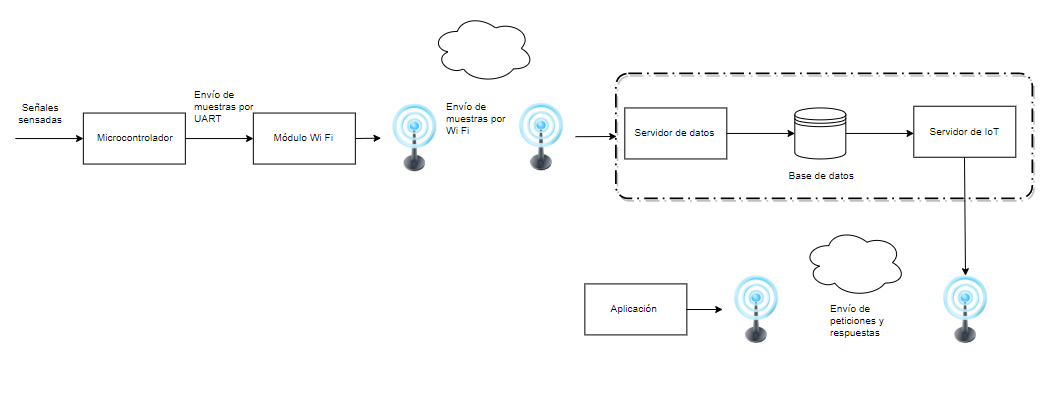
\includegraphics[scale=.3]{Capitulo3/img/diagramaBloques.png}
	\caption{Diagrama a bloques del sistema}
	\label{fig:diagrama_dispMonitoreo}
\end{figure}

\begin{itemize}
	\item Módulo de Microcontrolador.
	\item Módulo de Servidor.
	\item Módulo de Aplicación de usuario.
\end{itemize}

\paragraph{Módulo de Microcontrolador}
\begin{enumerate}[label=RF\arabic*.]
	\item Proporcionar un mecanismo de comunicación vía IIC desde el transductor MCP39F521 hacia el microcontrolador DSPIC30F4013.
	\item Proporcionar un mecanismo de comunicación vía UART desde el microcontrolador DSPIC30F4013 hacia el módulo Wi-Fi MIKROE-2542.
\end{enumerate}

\paragraph{Módulo de Servidor.}
\begin{enumerate}[label=RF\arabic*.]
	\setcounter{enumi}{12}
	\item Proporcionar un servicio para la recepción de los paquetes enviados por el módulo Wi-Fi MIKROE-2542 y su almacenamiento en un archivo de formato de texto.
	\item Proporcionar un servicio de comunicación vía HTTP para el envío de la información almacenada para dar respuesta a las peticiones realizadas por el usuario desde la aplicación móvil.  
\end{enumerate}

\paragraph{Módulo de Aplicación de usuario.}
\begin{enumerate}[label=RF\arabic*.]
	\setcounter{enumi}{16}
	\item Proporcionar un mecanismo para la vinculación entre la aplicación y el servidor.
	\item Proporcionar un servicio de comunicación vía HTTP para la generación de peticiones al servidor.
	\item Proporcionar un mecanismo para la visualización en tiempo real de la generación  de la energía producida por el sistema fotovoltaico.
	\item Proporcionar un mecanismo para la generación de estadísticas de la producción de energía por el sistema fotovoltaico.
	\item Informar por medio de notificaciones cuando el sistema fotovoltaico dejó de producir energía, así como al final del día notificar si se produjo más o menos energía que el promedio diario de producción.  
\end{enumerate}
\section{Requerimientos no funcionales}
A continuación, se presenta un listado con los requerimientos no funcionales que fueron identificados para el sistema:
\begin{enumerate}[label=RNF\arabic*.]
    \item Eficiencia: El sistema debe ser capaz de operar adecuadamente y responder a través de la aplicación móvil al usuario en a lo más 7 segundos.
	\item Escalabilidad: La arquitectura bajo la que es construido el sistema permite que este sea escalable y pueda expandirse hacia más funcionalidades.
	\item Seguridad: Los datos almacenados en el archivo de formato de texto correspondiente serán cifrados utilizando el algoritmo AES. **
	\item Usabilidad: La aplicación móvil cuenta con un diseño ergonómico y de fácil comprensión de tal forma que un usuario pueda utilizarla sin complicaciones, y a su vez con un tiempo de aprendizaje de a lo más dos horas.
	\item Tiempo de ejecución: Cuando se envíe una petición al servidor por parte de la aplicación móvil para mostrar la información de la energía censada, este debe responder en un tiempo máximo de 5 segundos. **
	\item Versiones de android: La aplicación móvil será desarrollada para versiones android igual o mayores a la versión 5.0.
	\item Tamaño: La aplicación móvil no podrá ocupar más de 700 mb de espacio en memoria interna del teléfono celular.
	\item Disponibilidad: El sistema debe tener una disponibilidad del 99,99\% de las veces en que un usuario intente hacer uso de las funcionalidades a través de la aplicación móvil. **
	\item Tolerancia a fallos: La probabilidad de falla del sistema no podrá ser mayor a 0,05\% y cuando se presente un error, este no tardará más de 15 minutos en restaurarse a un estado válido. **
	\item Concurrencia: La aplicación móvil debe soportar 1000 peticiones sin que el tiempo de respuesta por parte del servidor para todas ellas sea mayor a 10 segundos. **
\end{enumerate}
\section{Requerimientos técnicos}
Para utilizar la aplicación es necesario que los usuarios cuenten con ciertos requisitos en sus teléfonos móviles, dichos requisitos se enunciarán a continuación.
\subsection{Requerimientos mínimos de software del módulo de aplicación de usuario}
\begin{enumerate}
	\item Sistema Operativo: Android 5.0 Lollipop minSDKVersion 21 o superior.
\end{enumerate}
\subsection{Requerimientos mínimos de hardware del módulo de aplicación de usuario}
\begin{enumerate}
	\item Memoria RAM: 2GB
	\item Almacenamiento: Espacio libre mayor a 100 MB.
	\item Comunicación Wi-Fi IEEE 802.11 
	\item Procesador: Dual-Core de 1.2 GHz
\end{enumerate}
\section{Reglas de negocio}
Las reglas de negocio sirven para definir o restringir acciones que serán implementadas en funcionalidad. 
En la presente sección, se muestran las reglas de negocio del sistema.
\begin{enumerate}[label=RN\arabic*.]
    \item \label{RN1}
		\begin{description}
			\item[Nombre] RN1-Obtención de muestras del sistema fotovoltaico en tiempo real.
			\item[Tipo] Operación.
			\item[Objetivo] La obtención de mediciones del sistema fotovoltaico se realizará en tiempo real.
			\item[Descripción] La obtención de mediciones del sistema fotovoltaico dependerá del dispositivo de monitoreo empleado, en este caso, se trata del MCP39F521, y está determinada por la frecuencia de reloj de IIC de 400 Khz, sin embargo nuestro sistema trabajará a una frecuencia de 1 segundo.
    		\end{description}
    		
\item \label{RN2}
	\begin{description}
		\item[Nombre] RN2-Envío de muestras del sistema fotovoltaico en tiempo real.
		\item[Tipo] Operación.
		\item[Objetivo] Establecer el tiempo y frecuencia de envío de mediciones del microcontrolador por medio del módulo Wi-Fi.
		\item[Descripción] El envío de muestras del microcontrolador por medio del módulo Wi-Fi dependerá de la velocidad de transmisión UART entre el microcontrolador y el módulo, que es de 115200 baudios. Un baudio es el número de unidades de información transmitidas por segundo, que dependiendo de la configuración puede estar entre los 9600 a 11520 Bytes/Segundo, la frecuencia de envío de muestras hacia el servidor será de 1 segundo, obteniendo así una resolución de la unidad de generación de energía en Kilowatt Segundo para después ser convertida a Kilowatt Hora.
		\end{description}	
		
    \item \label{RN3}
		\begin{description}
			\item[Nombre] RN3-Creación de notificaciones por comportamiento inesperado.
			\item[Tipo] Habilitadora de acción.
			\item[Objetivo] Crear alertas que le informen al usuario el momento exacto en que el sistema fotovoltaico ha dejado de producir energía, el sistema ha dejado de obtener información de un nodo o el servidor no responde las peticiones.
			\item[Descripción] La alerta será creada y enviada como notificación al usuario de forma inmediata si y sólo si en el proceso de monitoreo para notificaciones se ha detectado alguno de los siguientes casos: la potencia activa de una muestra de un nodo es de 0 watts, si se pierde conexión con el microcontrolador o servidor.  
    		\end{description}
    		
\item \label{RN4}
		\begin{description}
			\item[Nombre] RN4-Calcular producción de energía histórica.
			\item[Tipo] Derivadora.
			\item[Objetivo] Calcular la producción de energía en el intervalo de tiempo especificado por cada nodo.
			\item[Descripción] La producción histórica de energía de un nodo es la suma de la potencia activa de cada una de las muestras obtenidas de acuerdo a la frecuencia de muestreo definida en la Regla de Negocio \ref{RN2}  
			Las opciones de periodos históricos son: última semana, mes actual, mensual, bimestral, anual y última década. Los reportes para los correspondientes periodos son:
			\\ Última semana: 
			\begin{itemize}
				\item La producción por cada día de la última semana, es decir, a partir del día actual, 6 días anteriores.
			\end{itemize}
			Mes actual: 
			\begin{itemize}
				\item La producción por cada día del mes actual.
			\end{itemize}
			Mensual: 
			\begin{itemize}
				\item La producción por cada mes del año actual.
			\end{itemize}
			Bimestral: 
			\begin{itemize}
				\item La producción en el periodo de tiempo comprendido del 1 de Enero al 28 o 29 de Febrero (dependiendo de si el año es bisiesto)
				\item La producción en el periodo de tiempo comprendido del 1 de Marzo al 30 de Abril
				\item La producción en el periodo de tiempo comprendido del 1 de Mayo al 30 de Junio
				\item La producción en el periodo de tiempo comprendido del 1 de Julio al 31 de Agosto
				\item La producción en el periodo de tiempo comprendido del 1 de Septiembre al 31 de Octubre
				\item La producción en el periodo de tiempo comprendido del 1 de Noviembre al 31 de Diciembre
			\end{itemize}
			Anual: 
			\begin{itemize}
				\item La producción en meses del año seleccionado.Se conservarán registros de los últimos 10 años.
			\end{itemize}
			Última década:
			\begin{itemize}
			\item La producción por año de los últimos 10 años.
			\end{itemize}
		\end{description}

\item \label{RN5}
		\begin{description}
			\item[Nombre] RN5-Agrupar muestras tomadas en un día por intervalos de producción.
			\item[Tipo] Derivadora.
			\item[Objetivo] Agrupar las muestras tomadas en un día por cada nodo en intervalos de producción tomando como referencia la máxima generación de potencia del sistema fotovoltaico. 
			\item[Descripción] Las muestras diarias de cada nodo serán agrupadas en los siguientes intervalos:
			\begin{itemize}
				\item Muestras mayores o iguales al 50\% de la máxima generación del sistema fotovoltaico.  
				\item Muestras menores que el 50\% y mayores o iguales al 20\% de la máxima generación del sistema fotovoltaico. 
				\item Muestras menores al 20\% de la máxima generación del sistema fotovoltaico. 
			\end{itemize}
		\end{description}

\item \label{RN6}
		\begin{description}
			\item[Nombre] RN6-Periodo de toma de muestras.
			\item[Tipo] Operación.
			\item[Objetivo] Establecer el periodo de tiempo en el que las muestras serán tomadas para cada nodo.
			\item[Descripción] Las muestras para obtener el resultado de la producción de energía comenzarán a tomarse a partir de las 0:00:00 hrs hasta las 23:59:59 hrs en la frecuencia indicada en la \ref{RN2} Adicionalmente se guardará cada minuto el valor de la potencia activa de cada nodo para la generación de la gráfica en tiempo real, dando un total de 1440 muestras diarias.		
		\end{description}
		
%Checar tipo
\item \label{RN7}
		\begin{description}
			\item[Nombre] RN7-Estándar de comunicación.
			\item[Tipo] Habilitadora de acción.
			\item[Objetivo] Establecer el estándar de comunicación entre microcontrolador-servidor y servidor-aplicación de usuario.
			\item[Descripción] El estándar de comunicación entre el servidor y la aplicación de usuario será por medio de TCP, y para la comunicación entre microcontrolador y servidor será por medio de UDP, ambos proporcionan la base para los productos con redes inalámbricas que hacen uso de la marca Wi-Fi.
		\end{description}
		
%Checar tipo		
\item \label{RN8}
		\begin{description}
			\item[Nombre] RN8-Patrón de intercambio de mensajes.
			\item[Tipo] Habilitadora de acción.
			\item[Objetivo] Establecer el patrón de intercambio de información entre módulos.
			\item[Descripción] El patrón de intercambio de información a utilizar entre módulos será petición-respuesta para el caso del protocolo TCP, para UDP solamente se hace el envío del paquete.
		\end{description}
		
%Después definir los datos exactos? o en req técnicos		
\item \label{RN9}
		\begin{description}
			\item[Nombre] RN9-Almacenamiento de datos de monitoreo.
			\item[Tipo] Operación.
			\item[Objetivo] Establecer el método de almacenamiento de la información.
			\item[Descripción] El almacenamiento en el servidor está limitado por la memoria externa con capacidad desde 8GB de espacio que le es agregada, por lo que usaremos una herramienta que trabaja con una cantidad de datos fija, sobreescribiendo la información cuando terminan e inician nuevamente los periodos definidos en la Regla de Negocio \ref{RN4}		\end{description}

%Preguntar request-reply si es RN8?

%Definí como tipo, preguntar si otra regla debemos poner el formato (bien conformado con un xsd)?
%Checar si será XML o JSON
\item \label{RN10}
		\begin{description}
			\item[Nombre] RN10-Formato de archivo para almacenamiento de datos.
			\item[Tipo] Estructura.
			\item[Objetivo] Definir el formato de archivo en que serán almacenados los datos sensados.
			\item[Descripción] El formato en que serán almacenados los datos sensados está definido por un archivo con extensión JSON, estos archivos estarán contenidos dentro de la carpeta que corresponde al número de sensor esclavo correspondiente y a su vez dentro de la carpeta con el número de serie del microcontrolador correspondiente, que está identificado por dos letras alfabéticas, por ejemplo, AC.		
		\end{description}
		
\item \label{RN11}
		\begin{description}
			\item[Nombre] RN11-Formato de datos de respuesta para la aplicación de usuario.
			\item[Tipo] Estructura.
			\item[Objetivo] Definir el formato de los datos que se enviarán como respuestas a las peticiones del cliente.
			\item[Descripción] El formato de los datos que se darán como respuesta del servidor a la aplicación móvil será en formato JSON.
			\end{description}
			
%Checar referencias a lo largo del documento		
\item \label{RN12}
		\begin{description}
			\item[Nombre] RN12-Agrupar muestras tomadas en un día por código de colores. 
			\item[Tipo] Derivadora.
			\item[Objetivo] Agrupar las muestras tomadas en un día por cada nodo de acuerdo a un color para ser representado en una gráfica.
			\item[Descripción] Las muestras tomadas en un día para la gráfica en tiempo real y la de ayer de acuerdo a la \ref{RN6} serán agrupadas de acuerdo al siguiente código de colores:
			\begin{itemize}
			    \item Muestras null: Estas muestras aparecen cuando el servidor es levantado por primera vez, por lo tanto no tiene las muestras completas del día. Se identificarán con el color gris.
			    \item Muestras de ayer: Estas muestras aparecen cuando por algún motivo una o más muestras no se sobreescriben con el valor del día de hoy, por lo tanto conservan el valor del día anterior. Se identificarán con el color azul.
			    \item Muestras perdidas: Estas muestras aparecen cuando el servidor no pudo leer la información del nodo en un momento en específico. Se identificarán con el color negro.
			    \item Mejores muestras: Estas muestras indican el valor más alto de potencia activa registrado durante el día. Se identificarán con el color morado.
			    \item Muestras mayores o iguales al 50\% de la máxima generación del sistema fotovoltaico. Se identificarán con el color verde  
				\item Muestras menores que el 50\% y mayores o iguales al 20\% de la máxima generación del sistema fotovoltaico. Se identificarán con el color naranja.
				\item Muestras menores al 20\% de la máxima generación del sistema fotovoltaico. Se identificarán con el color rojo.
			\end{itemize}
		\end{description}
	
\item \label{RN13}
		\begin{description}
			\item[Nombre] RN13-Número de registros de notificaciones.
			\item[Tipo] Restricción.
			\item[Objetivo] Definir la cantidad máxima de registros de notificaciones a conservar en la aplicación móvil.
			\item[Descripción] El número máximo de registros de notificaciones que se permitirán conservar en la aplicación móvil tiene que ser menor o igual a 100 notificaciones. El criterio para conservar las notificaciones dependerá únicamente del tiempo de llegada, es decir, se conservarán las notificaciones más recientes, sobreescribiendo el archivo cuando se llegue al límite.   
		\end{description}
		
\item \label{RN14}
		\begin{description}
			\item[Nombre] RN14-Formato de fecha de notificaciones.
			\item[Tipo] Estructura.
			\item[Objetivo] Definir el formato de fecha de las notificaciones para la aplicación móvil.
			\item[Descripción] El formato de fecha en que serán almacenadas las notificaciones del sistema en la aplicación móvil es: dd/mm/aa.
			Donde:
			\begin{itemize}
		 		\item dd = Corresponde al número de día del mes.
		 		\item mm = Corresponde al número de mes del año.
		 		\item aa = Corresponde al año
		    \end{itemize}
		\end{description}
		
\item \label{RN15}
		\begin{description}
			\item[Nombre] RN15-Formato de hora de notificaciones.
			\item[Tipo] Estructura.
			\item[Objetivo] Definir el formato de hora de las notificaciones para la aplicación móvil.
			\item[Descripción] El formato de hora en que serán almacenadas las notificaciones del sistema en la aplicación móvil es: hh:mm.
			Donde:
			\begin{itemize}
		 		\item hh = Corresponde a la hora del día en formato de 24 horas.
		 		\item mm = Corresponde al minuto de la hora.
		    \end{itemize}
		\end{description}
%Estipular cuantas muestras se tomaran por dia y bimestralmente y si se deshecharán,
%Tipo de archivo en el que se almacenarán los datos

\item \label{RN16}
		\begin{description}
			\item[Nombre] RN16-Formato de IP válido.
			\item[Tipo] Estructura.
			\item[Objetivo] Definir el formato IP válido para poder hacer la conexión con el servidor.
			\item[Descripción] El formato de IP válido será N.N.N.N
			Donde:
			\begin{itemize}
		 		\item N = número entero menor a 255 y mayor o igual a 0
		    \end{itemize}
		\end{description}

%Checar tipo 
\item \label{RN17}
		\begin{description}
			\item[Nombre] RN17-Tipos de peticiones de cliente a servidor.
			\item[Tipo] Habilitadora de acción.
			\item[Objetivo] Definir los tipos de peticiones que el usuario puede realizar desde la aplicación móvil a servidor.
			\item[Descripción] El usuario de la aplicación móvil puede realizar las siguientes peticiones al servidor.
			\begin{itemize}
		 		\item Connect: Esta petición se lanza cuando el usuario desea conectarse por primera vez al servidor.
		 		\item Set\_password: Esta petición se lanza cuando es el primer usuario en conectarse al servidor y tiene que establecer un correo electrónico y una contraseña.
		 		\item Get\_password: Esta petición se lanza cuando otros usuarios desean conectarse al servidor ingresando la contraseña establecida por el primer usuario.
		 		\item Forgot\_password: Esta petición se lanza cuando alguno de los usuario quiere recuperar la contraseña del servidor por medio del correo electrónico establecido por el primer usuario.
		 		\item Get\_info: Esta petición se lanza cuando se requiere obtener información sobre los microcontroladores y nodos conectados al servidor especificado.
		 		\item Get\_data: Esta petición se lanza cuando se requiere obtener el contenido de alguno de los archivos del nodo especificado.
		    \end{itemize}
		\end{description}


\item \label{RN18}
		\begin{description}
			\item[Nombre] RN18-Monitoreo para crear notificaciones.
			\item[Tipo] Habilitadora de acción.
			\item[Objetivo] Indicar bajo que condición se pueden obtener notificaciones del sistema.
			\item[Descripción] El usuario de la aplicación móvil puede permitir el monitoreo de los nodos en segundo plano, con el objetivo de poder recibir notificaciones cuando ocurran algunas de las condiciones establecidas en la \ref{RN3}, siempre y cuando lo solicite en la configuración de la aplicación.
		\end{description}
%checar		
\item \label{RN19}
		\begin{description}
			\item[Nombre] RN19-Monitoreo de nodos en la aplicación móvil.
			\item[Tipo] Habilitadora de acción.
			\item[Objetivo] Indicar bajo que condición se puede obtener información de los nodos en la aplicación móvil.
			\item[Descripción] El usuario de la aplicación móvil puede obtener información de los nodos sensores siempre y cuando estén conectados al servidor y las lecturas de las muestras sean almacenadas en los archivos del servidor.
		\end{description}
		
\item \label{RN20}
		\begin{description}
			\item[Nombre] RN20-Gestión de servidores en la aplicación móvil.
			\item[Tipo] Habilitadora de acción.
			\item[Objetivo] Indicar las opciones que tiene el usuario sobre los servidores registrados.
			\item[Descripción] El usuario de la aplicación móvil puede realizar las siguientes acciones en los servidores que ha registrado:
			\begin{itemize}
		 		\item Recuperar contraseña por medio del correo electrónico establecido por el primer usuario
		 		\item Editar el nombre del servidor.
		 		\item Eliminar el servidor para dejar de monitorearlo en la aplicación móvil.
		    \end{itemize}
		\end{description}

\item \label{RN21}
		\begin{description}
			\item[Nombre] RN21-Gestión de servidores.
			\item[Tipo] Habilitadora de acción.
			\item[Objetivo] Indicar las opciones que tiene el usuario sobre los servidores registrados.
			\item[Descripción] El usuario de la aplicación móvil puede realizar las siguientes acciones en los servidores que ha registrado:
			\begin{itemize}
		 		\item Recuperar contraseña por medio del correo electrónico establecido por el primer usuario
		 		\item Editar el nombre del servidor.
		 		\item Eliminar el servidor para dejar de monitorearlo en la aplicación móvil.
		    \end{itemize}
		\end{description}
		
\item \label{RN22}
		\begin{description}
			\item[Nombre] RN22-Tiempo de obtención de muestra actual en tiempo real.
			\item[Tipo] Operación.
			\item[Objetivo] Establecer la frecuencia con la que se enviarán peticiones al servidor para obtener el valor actualizado de la muestra de un nodo en tiempo real.
			\item[Descripción] El usuario de la aplicación móvil puede observar el valor actualizado de la muestra de producción en tiempo real de un nodo cada 2 segundos.
		\end{description}
		
\item \label{RN23}
		\begin{description}
			\item[Nombre] RN23-Tiempo de obtención de muestras de hoy en tiempo real.
			\item[Tipo] Operación.
			\item[Objetivo] Establecer la frecuencia con la que se enviarán peticiones al servidor para obtener la información actualizada del archivo que contiene las muestras de un nodo durante el día en curso.
			\item[Descripción] El usuario de la aplicación móvil puede observar el valor actualizado de las muestras de producción durante el día en curso de un nodo cada 1 minuto.
		\end{description}
		
		
		
		
\end{enumerate}



%\section{Descripción del software}
\subsection{Android}
Es un sistema operativo móvil desarrollado por Google; está basado en Linux, que junto con aplicaciones middleware está enfocado para ser utilizado en dispositivos móviles como teléfonos inteligentes, tables, Google TV y otros dispositivos.
A continuación, en la Tabla \ref{Tabla_android} se muestra una comparación entre distintos sistemas operativos para dispositivos móviles.
\begin{table}[H]
	\centering
	\begin{tabular}{|M{3.2cm}|M{3cm}|M{3cm}|M{3cm}|}
		\hline 
		\textbf{Características} & \textbf{Android} & \textbf{IOS} & \textbf{Windows Phone} \\ \hline
		Núcleo & Linux & XNU & Windows NT \\ \hline
		Arquitectura soportada & ARM, MIPS, x86 & ARM & ARM, Microsoft XNA \\ \hline
		Programado & C, C++ y Java & C, C++, Objective-c y Swift & XNA, NET, C\#, C, C++ y VB.NET \\ \hline
		Entorno de desarrollo & Android Studio & Xcode & Visual Basic \\ \hline
		Conectividad & GSM/EDGE, IDEN, CDMA, EV-DO, UMTS, Bluetooth, WiFi, LITE, HSDPA, HSPA+, NFC y WiMAX & WiFi.802.11AC, Bluetooth LE & WiFi 802.11b/g y Bluetooth \\ \hline
		Sincronización con la nube & Google Drive & iCloud & SkyDrive \\ \hline
		Tienda de aplicaciones & Google Play & App Store & Windows Phone Store \\ \hline
		Almacenamiento de datos & SQLite & SQLite & SQLite \\ \hline
		Navegador web & Chrome & Safari & Internet Explorer \\ \hline
		Tipo de interfaz & Iconos y widgets & Iconos & Baldosas animadas \\ \hline
	\end{tabular}
	\caption{Tabla comparativa de dispositivos móviles}
	\label{Tabla_android}
\end{table}

Al comprar las características de las distintas tecnologías para dispositivos móviles, se decidió utilizar Android debido a que existe una gran parte de la población que cuenta con un dispositivo con este sistema operativo, asimismo nos brinda mayores posibilidades de conectividad y un entorno de desarrollo más accesible debido a que es una tecnología OpenSource.


\subsection{Java}
Java es un lenguaje de programación y una plataforma informática comercializada por primera vez en 1995 por Sun Microsystems.\\
Es una tecnología que se usa para el desarrollo de aplicaciones que convierten a la Web en un elemento más interesante y útil.
Java permite jugar, cargar fotografías, chatear en línea, realizar visitas virtuales y utilizar servicios como, por ejemplo, cursos en línea, servicios bancarios en línea y mapas interactivos \citep{java}.
En la tabla \ref{tabla_lenguajes} se muestra una tabla comparativa entre tres distintos lenguajes de programación.
\begin{longtable}{|M{2.5cm}|M{3cm}|M{4.2cm}|M{4.3cm}|}
		\hline 
		\textbf{Lenguaje} & \textbf{Características} & \textbf{Ventajas} & \textbf{Desventajas} \\ \hline
		Java & Lenguaje orientado a objetos & \begin{itemize}
			\item Multiplataforma
			\item No existen problemas con la liberación de la memoria en el sistema.
			\item Cuenta con una amplia variedad de bibliotecas estándar.
		\end{itemize} &  \begin{itemize}
		\item Tiene un rendimiento menor comparado con los demas lenguajes de programación.
		\item Es necesario tener la maquina virtual de Java para poder ejecutar los programas.
		\item Es un lenguaje que evoluciona muy lentamente
	\end{itemize} \\ \hline
		C\# & Lenguaje de programación orientado a objetos & \begin{itemize}
			\item Declaración en el espacio de nombres
			\item Existe un rango más amplio y definido de tipos de datos.
			\item Propiedades: un objeto tiene intrínsecamente propiedades.
		\end{itemize} & \begin{itemize}
		\item Se necesita una versión reciente de VS.NET
		\item Se requiere Windows NT 4 o superior
	\end{itemize} \\ \hline
		Python & Lenguaje de programación interpretado y orientado a objetos & \begin{itemize}
			\item Tipado dinamico
			\item Facilidad de aprendizaje
			\item Sintaxis sencilla
		\end{itemize} & \begin{itemize}
		\item Al ser un lenguaje interpretado lo vuelve mas lento.
	\end{itemize} \\ \hline
	\caption{Tabla comparativa de diferentes lenguajes de programación}
	\label{tabla_lenguajes}
\end{longtable}
El lenguaje de programación que será utilizado en el presente proyecto será Java, debido a que el desarrollo de aplicaciónes moviles y web es mas sencillo. Ademas Java nos da la posibilidad de compilar una sola vez el proyecto y poder ejecutarlo en cualquier plataforma sin tener que recompilarlo de nuevo. Asimismo Java nos brinda seguridad, portabilidad y fiabilidad.
\subsection{Spring 4}
Spring Framework proporciona un completo modelo de programación y configuración para aplicaciones empresariales modernas basadas en Java, en cualquier tipo de plataforma de implementación.
Un elemento clave de Spring es el soporte de infraestructura en el nivel de la aplicación: Spring se centra en la "plomería" de las aplicaciones empresariales para que los equipos puedan enfocarse en la lógica empresarial a nivel de la aplicación, sin vínculos innecesarios con entornos de implementación específicos \citep{spring}.
\\
En la tabla \ref{tabla_frameworks} se muestra una tabla comparativa entre distintos frameworks.
\begin{longtable}{|M{3cm}|M{4.2cm}|M{4.2cm}|M{4.3cm}|}
	\hline 
	\textbf{Framework} & \textbf{Ventajas} & \textbf{Desventajas} \\ \hline
	Spring 4 & \begin{itemize}
		\item Lenguaje Java
		\item Fácil configuración
		\item Open source
		\item Estandarizado
	\end{itemize} &  \begin{itemize}
		\item Te atrae a que te adaptes al sistema.
	\end{itemize} \\ \hline
	Django & \begin{itemize}
		\item Desarrollo rápido
		\item Open source
		\item Fácil de aprender
		\item MVT
	\end{itemize} & \begin{itemize}
		\item Templates no tan robustos
		\item Se reinicia el servidor al recargar
		\item ORM no tan robusto
	\end{itemize} \\ \hline
	Node.js & \begin{itemize}
		\item Javascript
		\item High-performance
		\item Open source
		\item Asíncrono
	\end{itemize} & \begin{itemize}
		\item Limitado a una CPU
	\end{itemize} \\ \hline
	\caption{Tabla comparativa de diferentes frameworks}
	\label{tabla_frameworks}
\end{longtable}
Se eligió spring 4 como el framework para el desarrollo de la lógica del servidor, debido a que nos ofrece la posibilidad de utilizar el lenguaje Java, previamente elegido como lenguaje de programación del sistema, y nos brinda un soporte robusto de aplicaciones lo cual nos permite que el sistema funcione correctamente aun si este mismo crece.
\subsection{Servidor}
Un servidor es un ordenador u otro tipo de equipo informático encargado de suministrar información a una serie de clientes, que pueden ser tanto personas como otros dispositivos conectados a él. La información que puede transmitir es múltiple y variada: desde archivos de texto, imagen o vídeo y hasta programas informáticos, bases de datos, etc.
\textbf{Cloud Server}
Los cloud servers son unas alternativas para llevar la herramienta de los servidores al mundo virtual. La infraestructura en la nube se consigue gracias a la existencia de diversos servidores físicos controlados mediante un software, que es el encargado de virtualizar la plataforma.
\\Los servidores en la nube ofrecen a las empresas la posibilidad de tener un servidor a medida de sus necesidades, cuyos recursos y capacidades puedan ir incrementándose a conforme aumentan el tamaño y la actividad de la empresa, lo que permite un considerable ahorro para el presupuesto de las distintas corporaciones \citep{servidores}.
\\
En la tabla \ref{tabla_servidores} se tiene la comparación entre distintos cloud servers.
\begin{longtable}{|M{2.5cm}|M{4cm}|M{4.8cm}|M{3cm}|}
	\hline 
	\textbf{Cloud Server}& \textbf{Descripción} & \textbf{Características} & \textbf{Precio} \\ \hline
	Google Cloud Platform & Es una plataforma que ha reunido todas las aplicaciones de desarrollo web de Google. Google Cloud Platform es utilizada para crear soluciones a través de la tecnología almacenadas en la nube. &\begin{itemize}
		\item Permite la conexión por medio de SSH.
		\item Puedes desplegar el código directamente o mediante contenedores.
		\item Solo se paga por el tiempo utilizado.
		\item Maquinas virtuales personalizadas.
		\item Cuenta con un almacenamiento de hasta 624 GB por maquina.
		\item Proporciona almacenamiento en bloques en unidades de estado solido locales con encriptado permanente.
		\item Balanceo de carga global.
		\item Sistemas operativos: Debian, CentOS, CoreOS, SUSE, Ubuntu, Red Hat, FreeBSD o Windows 2008 R2, 2012 R2 y 2016
		\item Procesamiento por lotes.
	\end{itemize} &  Aproximadamente 0.1900 USD/hora \\ \hline
	Amazon Web Services & 
	Es una plataforma de servicios de nube que ofrece potencia de cómputo, almacenamiento de bases de datos, entrega de contenido y otra funcionalidad para ayudar a las empresas a escalar y crecer.
	&\begin{itemize}
		\item Instancias dedicadas: brindan acceso directo al procesador y a la memoria del servidor.
		\item Instancias de informática con GPU
		\item Instancias de E/S de alto desempeño: Ofrecen un desempeño de disco secuencia de hasta 16 GB/s
		\item Instancias de almacenamiento denso: Hasta 48 TB de almacenamiento.
		\item Volúmenes de almacenamiento en bloques persistente, de alta disponibilidad, constantes y de baja latencia
		\item Se paga por lo que se consuma
		\item Posibilidad de colocar las instancias en distintas ubicaciones.
		\item Auto Scaling
		\item Amazon Time Sync Service ofrece un origen de hora de alta precisión, fiabilidad y disponibilidad para los servicios de AWS
		\item Sistemas operativos: Amazon Linux, Windows Server 2012, CentOS 6.5, Debian.
	\end{itemize} & Aproximadamente 0,0832 USD por hora \\ \hline
	Heroku & Heroku es una plataforma en la nube basada en un sistema de contenedor administrado, con servicios de datos integrados y un poderoso ecosistema, para implementar y ejecutar aplicaciones modernas &\begin{itemize}
		\item Ejecuta las aplicaciones dentro de dynos:contenedores inteligentes en un entorno de tiempo de ejecución confiable y administrado.
		\item Soporta código escrito en Node, Ruby, Java, PHP, Pytho, Go, Scala y Clojure.
		\item Se puede implementar desde herramientas como Git, Github o sistemas de integración continua.
		\item Permite extender las aplicaciones con complementos.
		\item Sistema para escalar automáticamente las web dynos.
		\item Cuenta con métricas de la aplicación, alertas de umbral y escala automática.
		\item Seguridad
		\item Sistema operativo Linux
	\end{itemize} & Aproximadamente 7 USD por dyno/mes \\ \hline
	\caption{Tabla comparativa de cloud servers}
	\label{tabla_servidores}
\end{longtable}
El servicio a utilizar sera Google Cloud Platform debido a que conforme va creciendo el sistema nos ofrece el menor precio, ademas de que nos permite tener una conexión por medio de SSH y asimismo soporta el lenguaje que será utilizado para el desarrollo de la aplicación.
%\section{Descripción del hardware}
\subsection{Sensor}\label{sec:Sensor}
Para la realización del presente trabajo, es necesario medir la cantidad de gasolina que es cargada a un automóvil. Para ello, es necesario usar un dispositivo capaz de medir cuanto liquido (en este caso la gasolina) esta siento cargada al mismo en un determinado tiempo. Este tipo de dispositivos, son conocidos como caudalímetros \cite{CAUDALIMETRO}.

Un caudalímetro, es un instrumento que se usa para medir el caudal caudal de un fluido, existen diversos tipos, tales como caudalímetros mecánicos visuales, mecánicos de molino, electrónicos de molino, de turbina y de diferencial de presión. Todos ellos se diferencian por la forma en que funcionan internamente, sin embargo, el funcionamiento de estos es similar. Cada vez que el liquido pasa a través de ellos, estos liberan un pulso eléctrico, comúnmente equivalente al voltaje de la fuente con la que están siendo alimentados.

En la Tabla \ref{tabla_caudalimetros}, se observa una comparativa entre distintos caudalímetros, los cuales fueron considerados como opciones para el desarrollo del presente trabajo.
\begin{table}[H]
	\centering
	\begin{tabular}{|M{2cm}|M{2cm}|M{2cm}|M{2cm}|M{2cm}|M{1.7cm}|M{1.4cm}|}
		\hline
		\textbf{Nombre} & \textbf{Presión de agua} & \textbf{Flujo de entrada} & \textbf{Voltaje de funcionamiento} & \textbf{Tubo de entrada y salida} & \textbf{Salida de pulso de alta} & \textbf{Precio unitario (pesos)} \\ \hline
		LG16 Liquid Flow Meter Series & 20MPa\cite{LG16} & 5000 ul/min & 3.5-12V & 1/16'' o 1/8'' & 4.8V & N/E \\ \hline
		FS400A-G1 Flow Meter & 1.2 MPa\cite{FS400A-G1} & 1 a 60L/min & 5-24V & 1'' & $>$4.7V & \$348 \\ \hline
		FMG800 Series & 1.03MPa\cite{FMG800} & 0.145 L/s hasta 42L/s & 10-30V & 1'', 2'' y 3'' & Depende de la unidad & \$28,110 \\ \hline
		Optiflux 1000 & 4MPa - 12MPa\cite{OPTIFLUX} & N/E & N/E & 3/8'' - 6'' & N/E & \$25,719 \\ \hline
	\end{tabular}
	\caption{Comparación de caudalímetros}
	\label{tabla_caudalimetros}
\end{table}

Un elemento importante por considerar para la elección del caudalímetro a usar, es la conexión que este requiere para poder ser conectado tanto al depósito de combustible de un automóvil como a la pistola despachadora de una gasolinera.

No fue encontrado un estándar el cual indique el tamaño de la boquilla de las pistolas despachadoras de gasolina, pero tomando como referencia las medidas de las pistolas que se encuentran en venta en Internet\cite{PISTOLAS}, se estableció, que la medida estándar de la boquilla de las pistolas de despacho de gasolina, se encuentra entre 3/4'' y 1''.

El sensor seleccionado para el desarrollo del trabajo, es el caudalímetro \textit{FS400A-G1}, debido a que se ajustan sus características y su precio a las necesidades de la aplicación. Considerando que tiene una boquilla de 1'', requiere de un voltaje de alimentación bajo (5v), y soporta una presión de hasta 1.2MPa, teniendo como referencia, que aproximadamente la presión de la bomba de gasolina es cercana a los 0.344MPa\cite{PISTOLA}.


\subsection{Microcontrolador}\label{sec:micro}
Un microcontrolador contiene todos los componentes que le permiten operar de forma independiente,
y ha sido diseñado en particular para tareas de monitoreo y/o control. En consecuencia,
Además del procesador, incluye memoria, varios controladores de interfaz, uno o
más temporizadores, un controlador de interrupción y, por último, pero no menos importante, pines de E/S de propósito general,
lo que le permite interactuar directamente con su entorno. Los microcontroladores también incluyen operaciones de bits\cite{Micro}.
\\
En la tabla \ref{Tabla_comparativa_microcontroladores} se tiene la compración entre distintos microcontroladores, los cuales fueron considerados para utilizarse en el presente trabajo terminal. 
\begin{table}[H]
	\centering
	\begin{tabular}{|M{3.2cm}|M{1cm}|M{1.3cm}|M{2cm}|M{1.7cm}|M{1.7cm}|M{2cm}|}
		\hline 
		\textbf{Microcontrolador} & \textbf{Flash (KB)} & \textbf{SRAM (Byte)} & \textbf{EEPROM (Byte)} & \textbf{I/O Pins}& \textbf{A/D (Canales)}& \textbf{Interfaces}\\ \hline
		ATMega8535 & 8 & 512 & 512 & 32 & 10 & SPI,  USART \\ \hline
		ATMega16 & 16 & 1024 & 512& 32 & 8& JTAG, SPI, IIC \\ \hline
		ATtiny15L & 1 & - & 64 & 6 & 4 & SPI \\ \hline
		DSPIC30F4013 & 48 & 2048 & 1024 & 16 & 12 & SPI, UART, IIC, CAN \\ \hline
	\end{tabular}
	\caption{Tabla comparativa microcontroladores}
	\label{Tabla_comparativa_microcontroladores}
\end{table}
El microcontrolador a utilizar será el ATMega16 debido a que nos proporciona dos interfaces de comunicación serial las cuales serán importantes en el envío de los datos por medio del módulo Bluetooth, asimismo nos ofrece una mayor capacidad de memoria Flash y SRAM. Otro factor importante para elegir este microcontrolador fue que las herramientas de programación para este dispositivo son compatibles con los sistemas operativos más recientes lo cual nos permite hacer simulaciones del funcionamiento de nuestro código antes de tenerlo programado en el dispositivo.  

\subsection{Comunicación inalámbrica}\label{sec:bluetooth}
Bluetooth: \\
Bluetooth es una tecnología de conectividad inalámbrica de baja potencia que se utiliza para transmitir audio, transferir datos y transmitir información entre dispositivos. Hay dos sabores de la tecnología Bluetooth, velocidad básica / velocidad de datos mejorada (BR / EDR) y baja energía (LE)\cite{Bluetooth}. 
\newline
WiFi:\\
WiFi es la abreviatura o el nombre comercial de Wireless Fidelity  y, como su nombre lo indica, es un sistema de conexión de ordenadores completamente inalámbrico, que permite a sus usuarios compartir y transferir información utilizando ondas de radio, es decir, sin utilizar cableado alguno.
\\
De esta manera, podemos mantener comunicaciones entre ordenadores, portátiles, móviles y otros dispositivos que cuenten con tecnología de recepción inalámbrica, facilitando enormemente las comunicaciones, incluso en lugares abiertos lejos de nuestras casas y oficinas.
Las redes WiFi por lo general son de libre acceso, a menos que estén protegidas mediante contraseñas, lo cual, indicaría que son unas redes privadas utilizadas para conexiones con redes locales (LAN)\cite{WiFi}.
\\
En la tabla \ref{Comparacion_Conexiones} se muestran las características que tiene cada uno de los modos de conexión.
\begin{table}[H]
	\centering
	\begin{tabular}{|M{4cm}|M{4cm}|M{4cm}|}
		\hline
		\textbf{Característica} & \textbf{Bluetooth} & \textbf{WiFi} \\ \hline
		Frecuencia & 2.4GHz & 2.4,3.6,5 GHz \\ \hline
		Costo & Bajo & Alto \\ \hline
		Ancho de banda & 800Kbps & 11Mbps \\ \hline
		Dispositivos que lo utilizan & Dispositivos móviles, mouse, teclado, computadoras,etc. & Dispositivos móviles, computadoras, TV,etc. \\ \hline
		Requerimientos de hardware & Adaptador bluetooth entre los dispositivos conectados. & Adaptadores inalámbricos en todos los dispositivos de red o puntos de acceso. \\ \hline
		Rango & 5-30 metros & 32 metros en interiores y 95 metros en exteriores \\ \hline
		Consumo de energía & Bajo & Alto \\ \hline
		Factibilidad de uso & Sencillo de utilizar, se pueden conectar hasta 7 dispositivos a la vez. & La dificultad de implementación aumenta debido a que se requiere configurar el hardware y software. \\ \hline
		Latencia & 200 ms & 150 ms \\ \hline
	\end{tabular}
\caption{Tabla comparativa de comunicación inalámbrica}
\label{Comparacion_Conexiones}
\end{table}
Debido a que la distancia requerida para realizar el envió de datos entre el microcontrolador y el dispositivo móvil es corta, el costo que el dispositivo tiene, y a que cuenta con una implementación sencilla se decidió utilizar la conexión inalámbrica de bluetooth para realizar la comunicación.
\newline
Tras definir el tipo de comunicación es necesario elegir el dispositivo que sera utilizado, por tal motivo en la tabla \ref{Comparacion_DispBluetooth} se muestran las características con las que cuentan dos distintos tipos de modulo Bluetooth.
\\
\begin{table}[H]
	\centering
	\begin{tabular}{|M{4cm}|M{4cm}|M{4cm}|}
		\hline
		\textbf{Característica} & \textbf{HC-05} & \textbf{HC-06} \\ \hline
		Modo de configuración & Maestro/Esclavo/Esclavo con autoconexión. & Esclavo \\ \hline
		Frecuencia & 2.4GHz & 2.4GHz \\ \hline
		Modulación & GFSK & GFSK \\ \hline
		Potencia de emisión & $\leq$ 4dBm Clase 2 & $\leq$ 6dBm Clase 2 \\ \hline
		Alcance & 5m a 10m & 5m a 10m \\ \hline
		Velocidad & Asincrónica: 2.1 Mbps (max.)/160 kbps, sincrónica: 1 Mbps/1 Mbps & Asincrónica: 2 Mbps (max.)/160 kbps, sincrónica: 1 Mbps/1 Mbps \\ \hline
		Consumo de corriente & 50mA & 30 mA a 40 mA \\ \hline
		Voltaje de operación & 3.6 V a 6 V. & 3.6 V a 6 V \\ \hline
		Pines & Módulo montado en tarjeta con regulador de voltaje y 6 pines suministrando acceso a VCC, GND, TXD, RXD, KEY y status LED (STATE) & Módulo montado en tarjeta con regulador de voltaje y 4 pines suministrando acceso a VCC, GND, TXD, y RXD \\ \hline
		Precio & \$145 pesos & \$140 pesos\\ \hline
	\end{tabular}
	\caption{Tabla comparativa de dispositivos bluetooth}
	\label{Comparacion_DispBluetooth}
\end{table}
El dispositivo bluetooth a utilizar es el módulo bluetooth HC-05 ya que este tiene el modo de configuración como maestro-esclavo lo cual se ajusta a las necesidades del trabajo, ademas de que el precio es accesible y no tiene mucha variación con respecto al HC-06.

%\section{Herramientas de desarrollo del sistema}
\subsection{Herramientas de desarrollo de software}
Las siguientes herramientas son usadas para el desarrollo del software del sistema:
\begin{itemize}
	\item MySQL 5.7.19: La base de datos que se usará para el desarrollo del sistema es una base de datos relacional SQL, por lo cual es necesario usar un Sistema Gestor de Base de Datos SQL, 
	\item Eclipse 4: Para el desarrollo, se usará el framework para desarrollo web para Java Spring 4.0. El entorno de desarrollo integrado Eclipse permite un desarrollo ágil para la construcción de aplicaciones basadas en este framework.
	\item Android Studio: Debido a que la aplicación móvil estará desarrollada para el sistema operativo Android, es necesario utilizar una herramienta que nos permita realizarla, por tal motivo se utilizará el IDE oficial para su desarrollo.
\end{itemize}
\subsection{Herramientas de desarrollo de hardware}
Las siguientes herramientas son usadas para el desarrollo del hardware del sistema:
:
\begin{itemize}
	\item Atmel Studio 7.0: Es necesario contar con un IDE que nos permita desarrollar y probar el código que sera utilizado en la programación del microcontrolador, por tal motivo se utilizara Atmel Studio 7.0 ya que nos brinda una interfaz amigable para la programación del microcontrolador y cuenta con soporte para el microcontrolador AtMega16, ademas nos permite realizar pruebas del funcionamiento del código escrito al visualizar los datos de cada uno de los puertos del microcontrolador.
	\item Proteus 8: Para realizar los diagramas del hardware del sistema se utilizara el software Proteus, el cual nos permite simular el funcionamiento del circuito y nos proporciona una gran diversidad de componentes necesarios para realizar el diseño del hardware.
\end{itemize}


\section{Metodología}

\textbf{Metodología en V}\\
Para el desarrollo del sistema se tomará como base la metodología en V. 
Elegimos esta metodología debido a que nuestro sistema se compone tanto de software como de hardware, por lo que las etapas que la conforman se adecúan perfectamente para el desarrollo de esta clase de sistemas como a continuación se explicará. \\
La metodología indica que se debe de partir de la especificación de requisitos tanto para software como para hardware, en esta etapa se definen los requerimientos funcionales, técnicos y no funcionales, trazando un plan para el diseño del sistema mediante casos de uso, comprendiendo las limitaciones, identificando el impacto del mismo y previendo posibles cambios. En la siguiente etapa se realiza un diseño de alto nivel con base en la información recogida sobre requisitos y análisis, permitiendo obtener un diseño y una visión general del sistema. 
A continuación, se realiza un diseño en detalle, donde veremos al sistema de manera modular, en nuestro caso contamos con un total de tres módulos, teniendo así la ventaja de rediseñar un módulo en específico, hacer cambios de manera efectiva y reducir costos por modificaciones futuras. Posteriormente, el diseño es implementado con el lenguaje de programación elegido para cada módulo, obteniendo programas ejecutables capaces de ofrecer la funcionalidad esperada. A su vez, cada módulo va a ser sometido a pruebas para validar el análisis y diseño previamente realizado \citep{Metodologia1}.
\\
Las pruebas de cada nivel son descritas a continuación:

\begin{itemize}

    \item Pruebas unitarias/modulares: Estas pruebas comprueban que todas las funcionalidades especificadas en el diseño del componente sean correctas y cubiertas, estas pruebas son realizadas por el desarrollador del componente.
    
    \item Pruebas de integración/interfaz: Una vez que los módulos han sido probados de manera unitaria, se procede a probar su funcionalidad de manera conjunta, estas pruebas están enfocadas a resolver los siguientes supuestos:
    
    \begin{itemize}
        \item Que espera un componente de otro componente, en término de servicios.
        \item Como es que estos servicios serán solicitados.
        \item Como es que estos servicios serán entregados.
        \item El manejo de errores por condiciones inesperadas.
    \end{itemize}
    
    Las pruebas deben corroborar el correcto funcionamiento de todas las interfaces entre componentes, al tener todos los componentes y sus interfaces terminados, tendremos como resultado el sistema completo, estas pruebas pueden ser realizadas por el desarrollador del componente.
    
    \item Pruebas del sistema: Una vez el sistema ha sido construido, debe ser probado contra las especificaciones del sistema para comprobar que cubra las funcionalidades requeridas.\\
    Esta parte se enfoca en probar el sistema de manera monolítica y debe incluir las pruebas para validar los requerimientos no funcionales.

    \item Pruebas de validación: similar a las pruebas del sistema, pero hay un cambio en el enfoque, ya que éstas comprueban que el sistema cumple con lo requerido, además las pruebas son realizadas por el usuario final del sistema.

\end{itemize}

\begin{figure}[H]
	\centering
	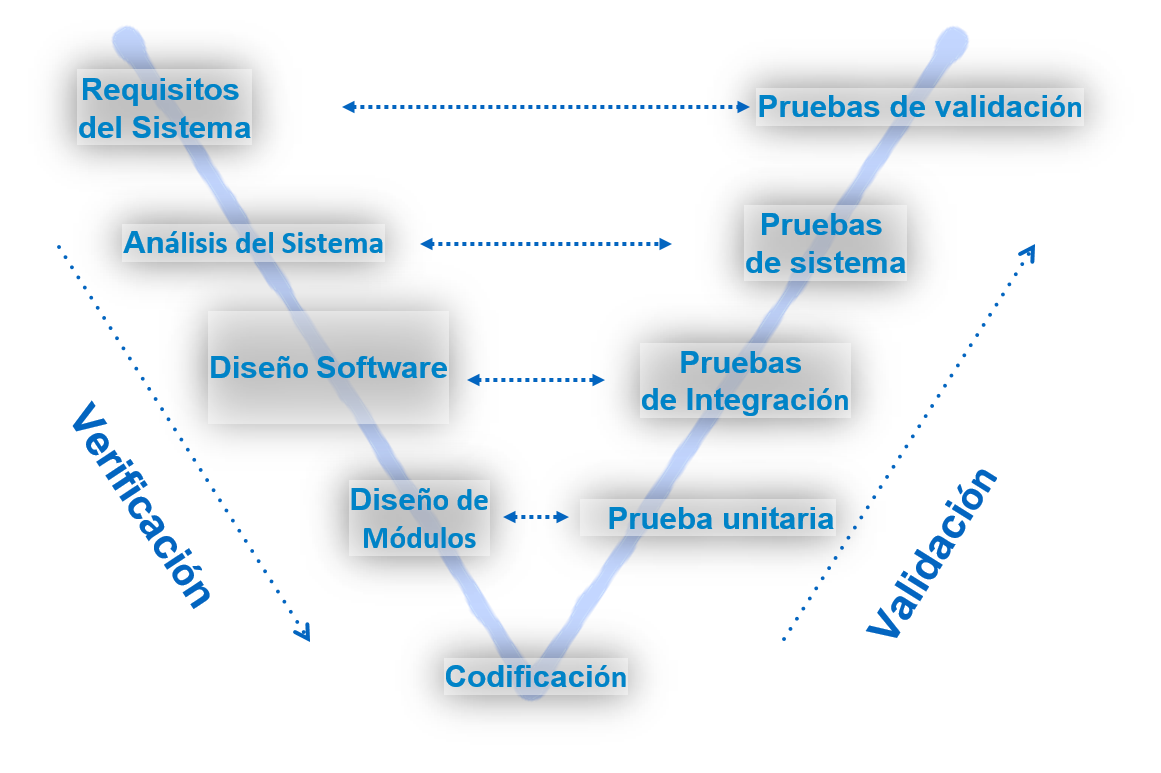
\includegraphics[scale=.5]{Capitulo3/img/vmodel.png}
	\caption{Metodología en V}
	\label{fig:ModeloIncremental}
\end{figure}


\section{Costo de desarrollo}
En esta sección presentamos el costo estimado de desarrollo del proyecto. \\
Es importante señalar que la estimación del costo de desarrollo se realizó tomando en cuenta los precios de los componentes utilizados para la parte de hardware \citep{MarcoTeorico5}, \citep{PlacaMCP}, \citep{PrecioDSPIC}, \citep{PrecioRasp} así como la parte correspondiente al desarrollo de software la cual abarca el desarrollo del servidor y la aplicación móvil de usuario, tomando como base el sueldo promedio mensual de un ingeniero en sistemas en México \citep{SalarioPromedio}.\\
%referencias de info de precios

En la %poner refernecia tabla
se enlistan los conceptos que forman parte de la estimación, así como algunos detalles.
%Colocar imagen de tabla excel







%%%%%%%%%%%%%%%%%%%%%%%%%%%%%%%%%%%%%%%%%%%%%%%%%%%%%%%%%%%%%%%%%%%%%%%%%
%           Capítulo 4: Diseño del Sistema                   %
%%%%%%%%%%%%%%%%%%%%%%%%%%%%%%%%%%%%%%%%%%%%%%%%%%%%%%%%%%%%%%%%%%%%%%%%%

\chapter{Diseño del sistema}\label{chapter4}

\section{Diagrama del proceso general del sistema}
En la Figura \ref{fig:proceso_general} se observa el diagrama del proceso general del sistema.
\begin{figure}[H]
	\centering
	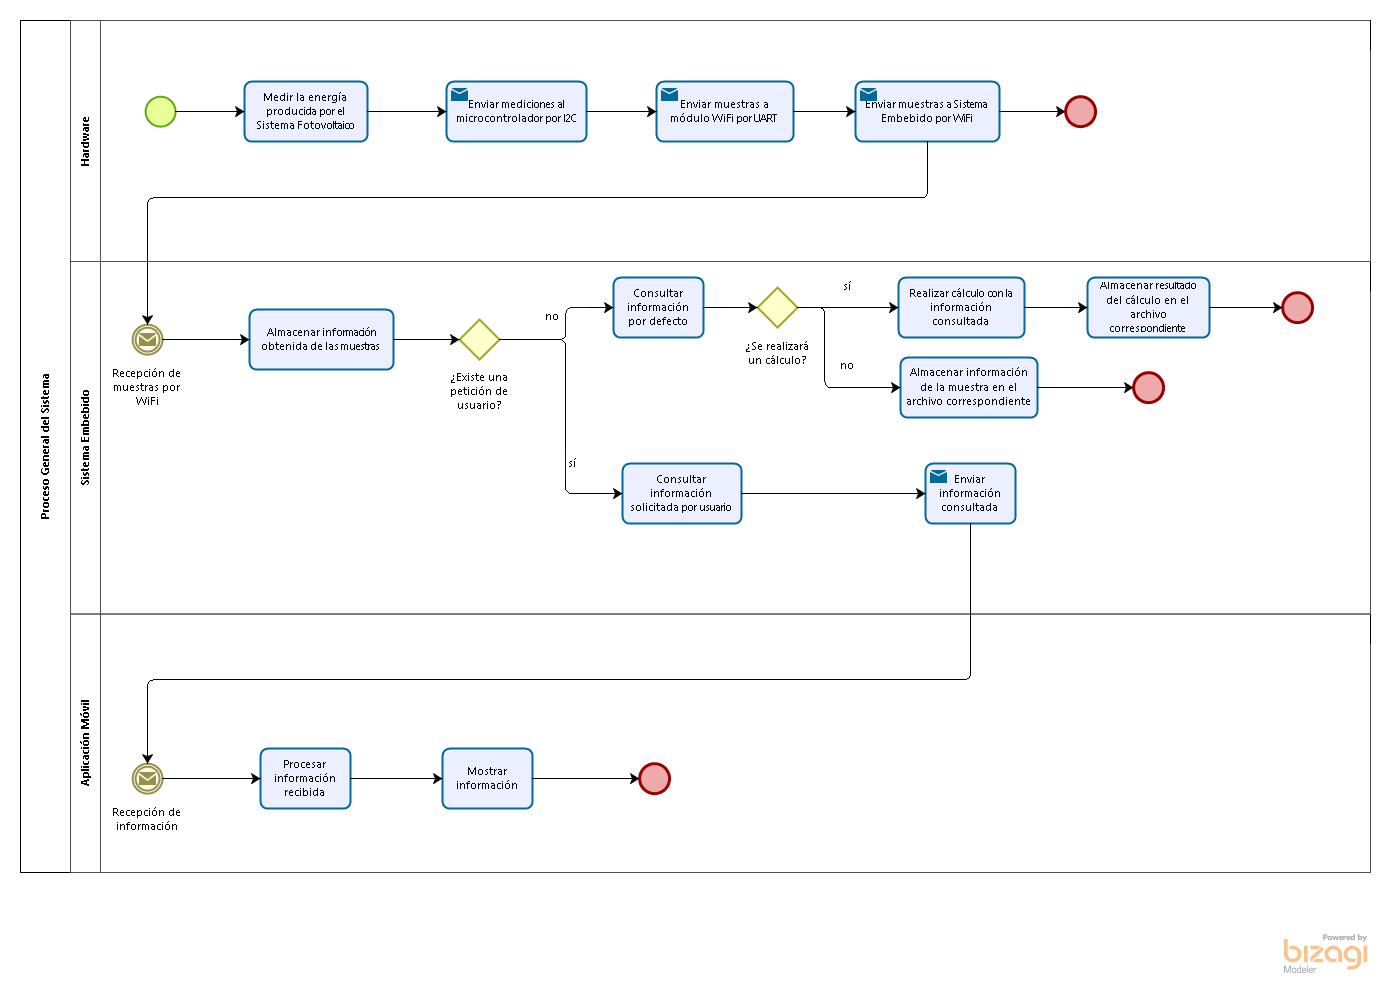
\includegraphics[scale=.35]{Capitulo4/images/procesoGeneral}
	\caption{Diagrama del proceso general del sistema}
	\label{fig:proceso_general}
\end{figure}
%\section{Arquitectura general del sistema}
En la Figura \ref{fig:arquitectura_sistema} se observa un diagrama de la arquitectura general del sistema.
\begin{figure}[H]
	\centering
	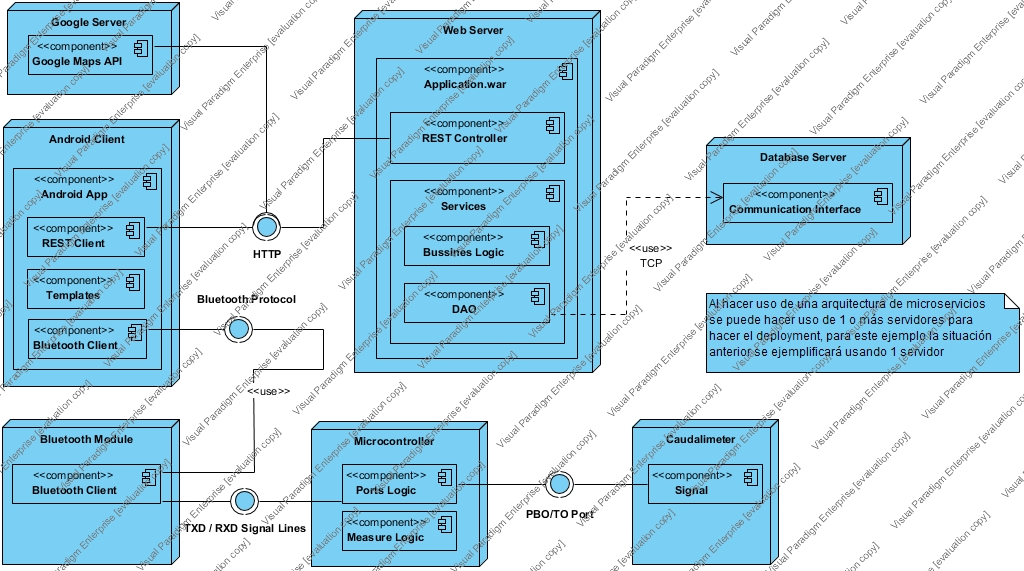
\includegraphics[scale=.44]{Capitulo4/images/arquitectura_sistema}
	\caption{Arquitectura general del sistema}
	\label{fig:arquitectura_sistema}
\end{figure}
%\section{Diagrama de clases}
En la Figura \ref{fig:diagrama_clases} se observa el diagrama de clases del sistema.
\begin{figure}[H]
	\centering
	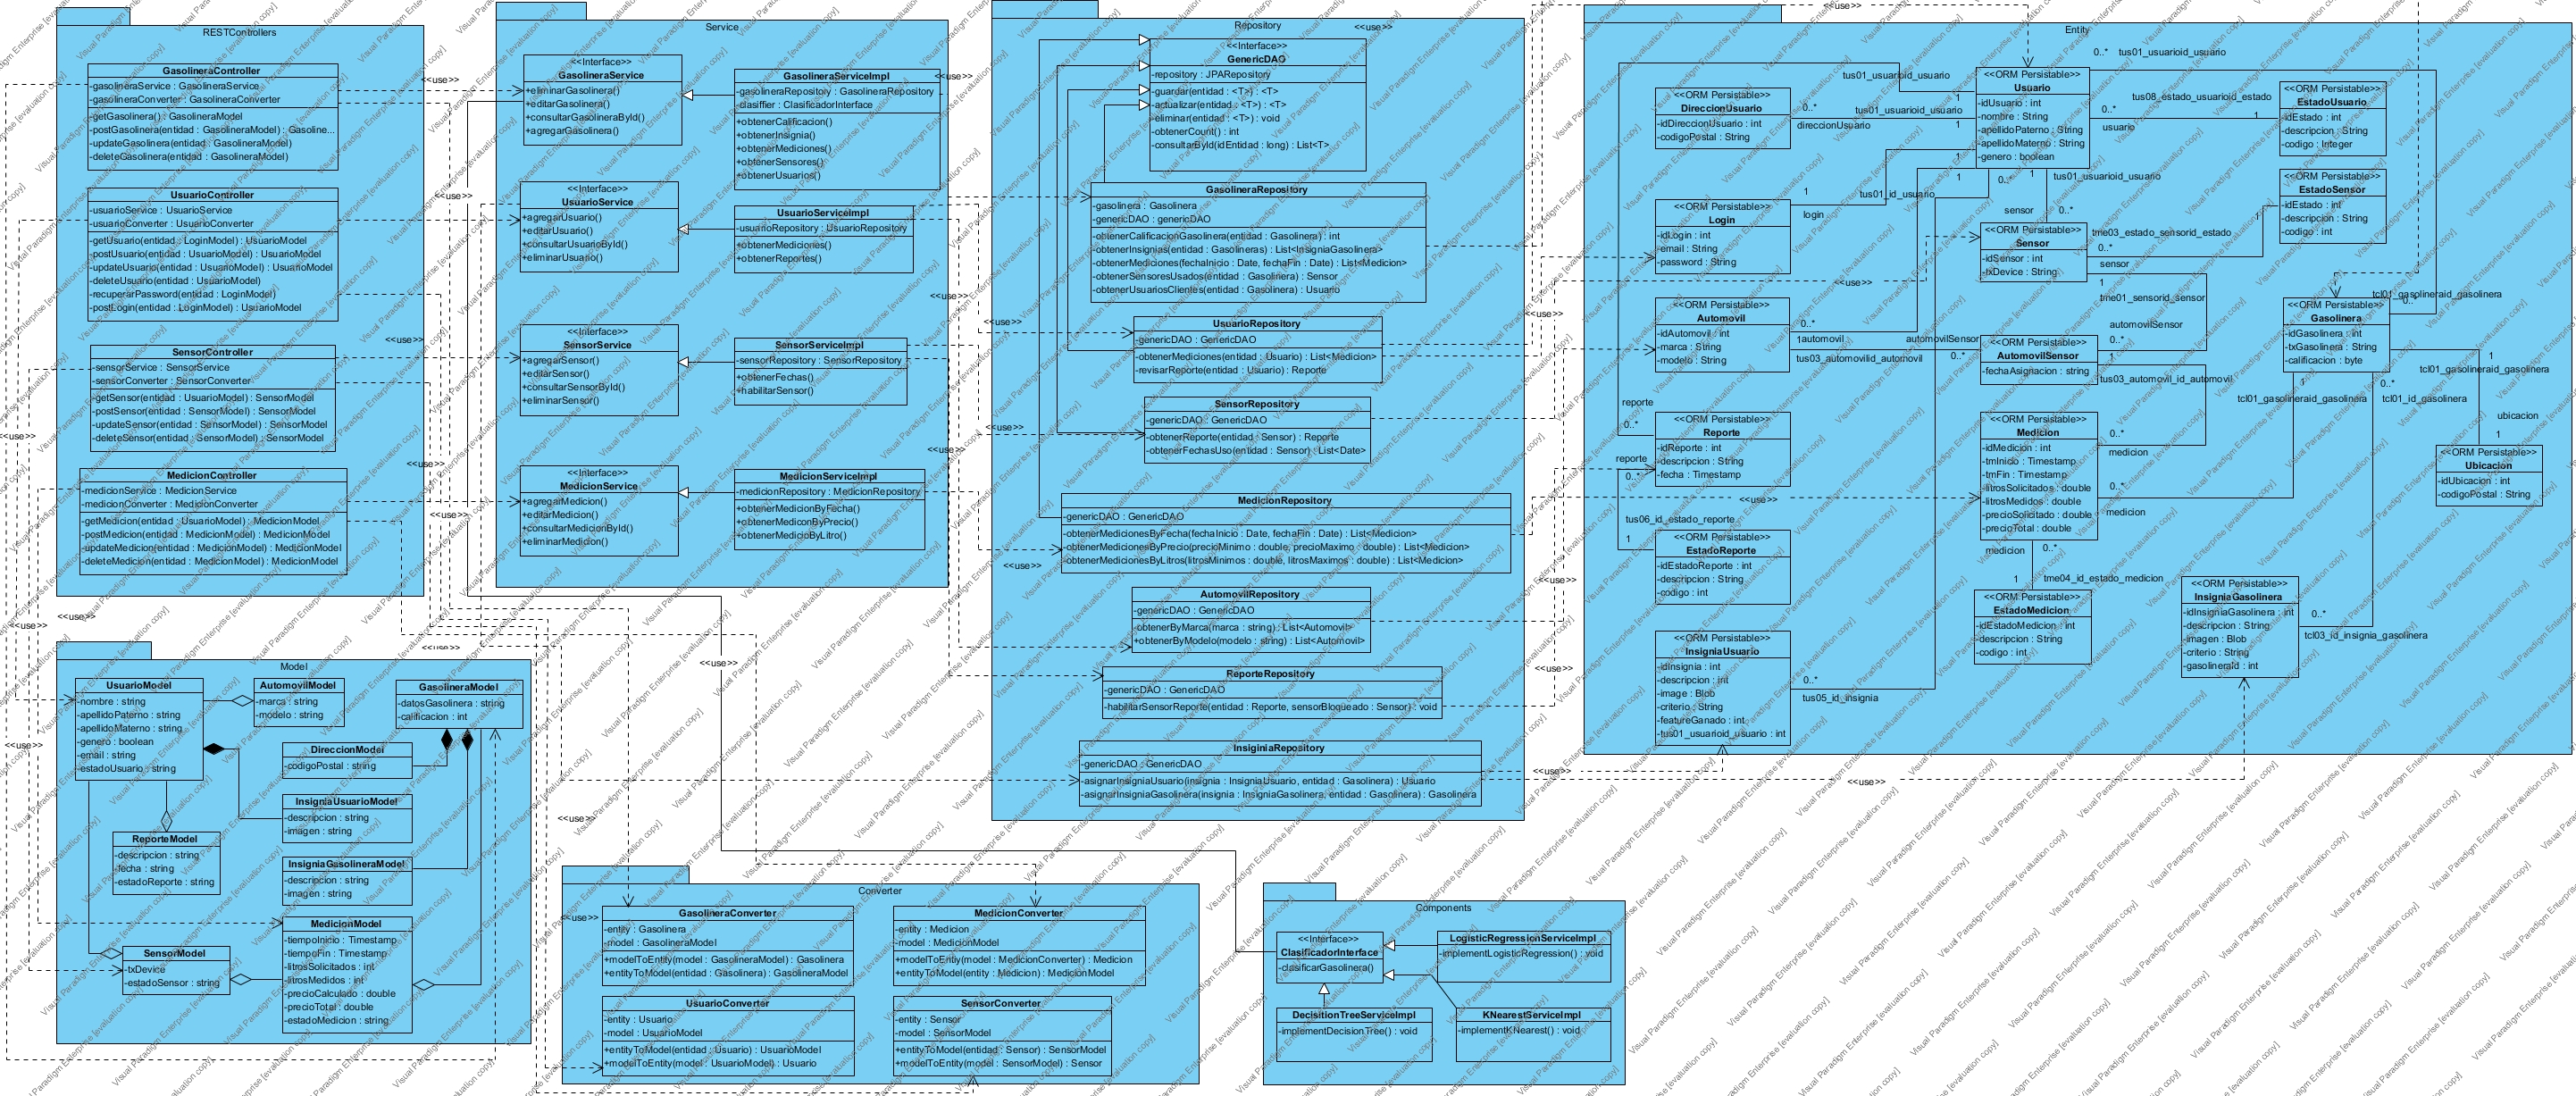
\includegraphics[scale=.21, angle=90]{Capitulo4/images/Clases}
	\caption{Diagrama de clases}
	\label{fig:diagrama_clases}
\end{figure}
\section{Modelo de información del sistema}
En la Figura \ref{fig:Base_ServidorEmbebido} se observa un diagrama del modelo de información correspondiente al servidor embebido, se puede observar que las tablas no se encuentran relacionadas, esto es debido a que la información que almacenan no está ligada de ninguna forma con el resto, a pesar de que los registros de algunas tablas sirvan para calcular los registros de otras.
\begin{figure}[H]
	\centering
	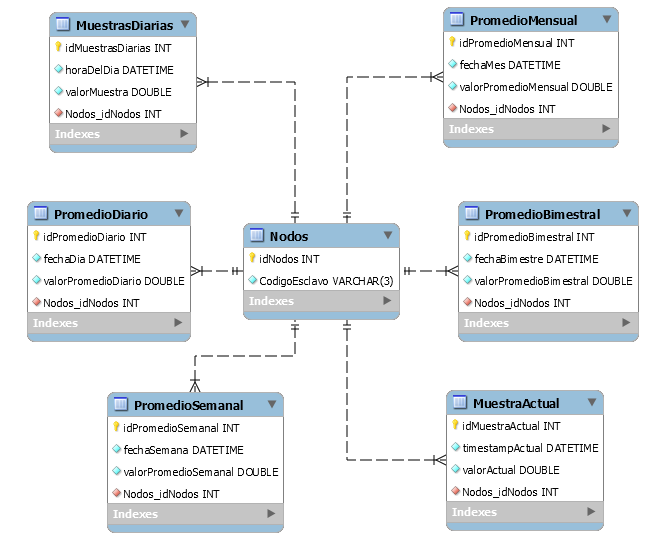
\includegraphics[scale=1.26]{Capitulo4/images/Base_ServidorEmbebido.PNG}
	\caption{Modelo de información del Servidor Embebido}
	\label{fig:Base_ServidorEmbebido}
\end{figure}

A continuación en la Figura \ref{fig:Base_AplicacionUsuario} se muestra el diagrama del modelo de información correspondiente a la aplicación de usuario, en donde se puede observar que únicamente se almacenará en la aplicación las notificaciones y los servidores que den respuesta a las peticiones de la aplicación de usuario, la relación entre tablas nos indica que muchas notificaciones pueden pertenecer a un mismo servidor.

\begin{figure}[H]
	\centering
	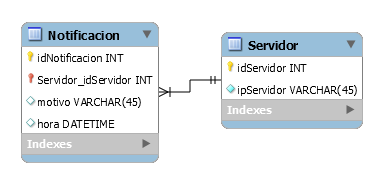
\includegraphics[scale=1.26]{Capitulo4/images/Base_AplicacionUsuario.PNG}
	\caption{Modelo de información de la aplicación de usuario}
	\label{fig:Base_AplicacionUsuario}
\end{figure}
%\section{Hardware}
En la imagen \ref{fig:circuito} se muestra el circuito que será utilizado para realizar la medición del flujo de gasolina y la comunicación por medio de bluetooth a la aplicación móvil.
\\
\begin{figure}[H]
	\centering
	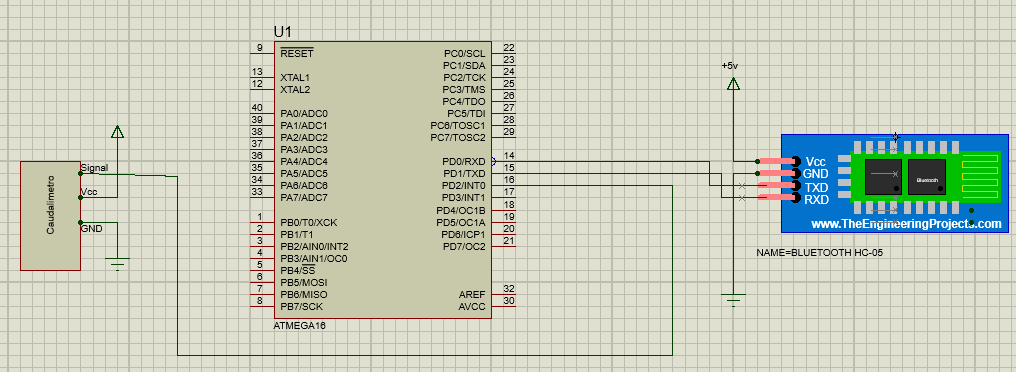
\includegraphics[width=1\textwidth]{Capitulo4/hardware/images/Caudalimetro}
	\caption{Circuito del sensor y comunicación}
	\label{fig:circuito}
\end{figure}

%\input{Capitulo4/hardware/submodulos/medicion/principal}
%\input{Capitulo4/hardware/submodulos/microcontrolador/principal}
%\input{Capitulo4/hardware/submodulos/comunicacion/principal}
\section{Hardware}
En la imagen \ref{fig:circuito} se muestra el circuito que será utilizado para realizar la medición del flujo de gasolina y la comunicación por medio de bluetooth a la aplicación móvil.
\\
\begin{figure}[H]
	\centering
	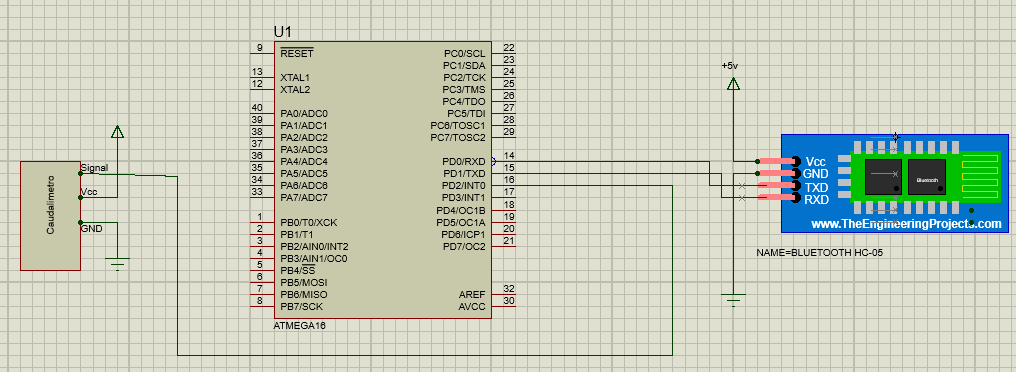
\includegraphics[width=1\textwidth]{Capitulo4/hardware/images/Caudalimetro}
	\caption{Circuito del sensor y comunicación}
	\label{fig:circuito}
\end{figure}

%\input{Capitulo4/hardware/submodulos/medicion/principal}
%\input{Capitulo4/hardware/submodulos/microcontrolador/principal}
%\input{Capitulo4/hardware/submodulos/comunicacion/principal}
\section{Software}

%\subsection{Diagrama de paquetes}
%En la Figura \ref{fig:dcu-general} se muestra el diagrama de paquetes del sistema.
%\begin{figure}[H]
%	\centering
%	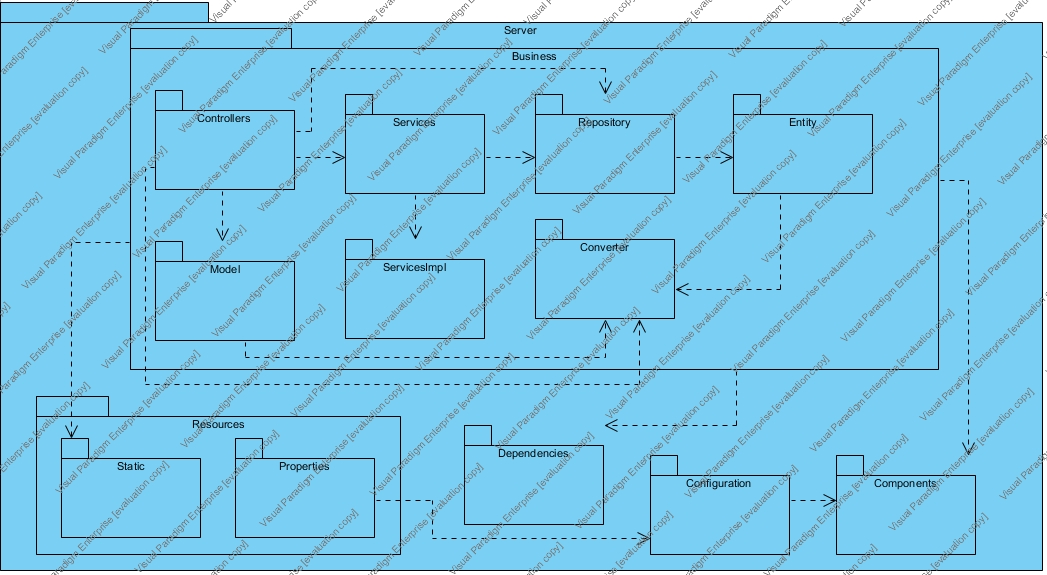
\includegraphics[scale=.198]{Capitulo4/images/Paquetes}
%	\caption{Diagrama de paquetes del sistema}
%	\label{fig:diagrama_paquetes}
%\end{figure}
%\subsection{Diagrama de casos de uso general}
%En la Figura \ref{fig:dcu-general} se muestra el diagrama general de casos de uso de todo el sistema.
%\begin{figure}[H]
%	\centering
%	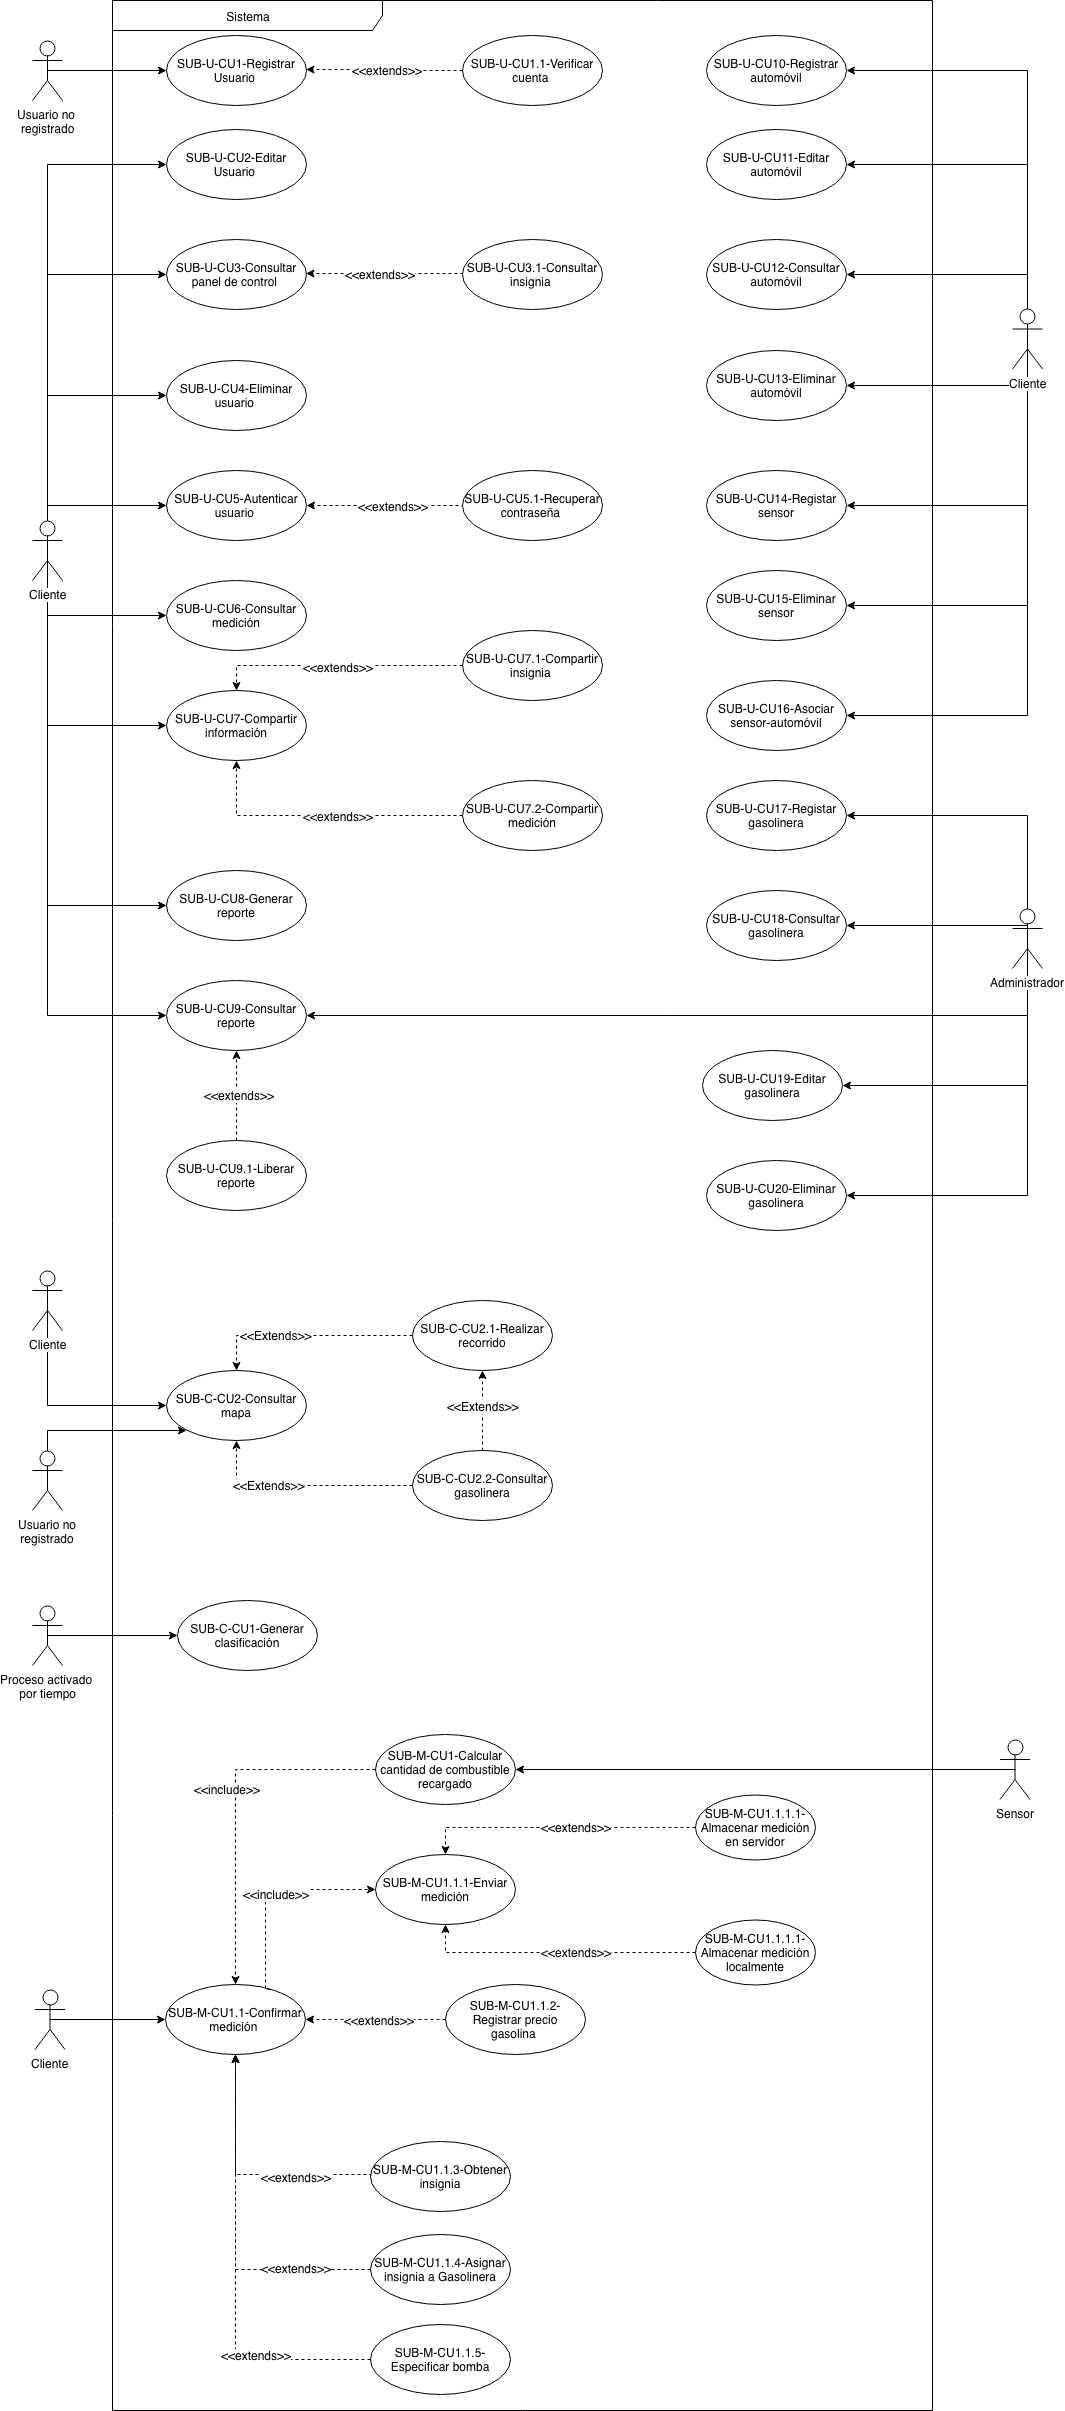
\includegraphics[scale=.198]{Capitulo4/software/submodulos/images/dcu}
%	\caption{Diagrama de casos de uso general}
%	\label{fig:dcu-general}
%\end{figure}
\input{Capitulo4/software/submodulos/mediciones/principal}
\newpage
\input{Capitulo4/software/submodulos/usuarios/principal}
\newpage
\input{Capitulo4/software/submodulos/clasificacion/principal}


\subsection{Menús de usuario}
\input{Capitulo4/software/menus}

\subsection{Interfaces de usuario}
%%%Mediciones
\input{Capitulo4/software/submodulos/mediciones/iu/sub-m-iu1_1}
\input{Capitulo4/software/submodulos/mediciones/iu/sub-m-iu1_1_2}
\input{Capitulo4/software/submodulos/mediciones/iu/sub-m-iu1_1_3}
\input{Capitulo4/software/submodulos/mediciones/iu/sub-m-iu1_1_4}
\input{Capitulo4/software/submodulos/mediciones/iu/sub-m-iu1_1_5}
%%%Usuarios
\input{Capitulo4/software/submodulos/usuarios/iu/sub-u-iu1}
\input{Capitulo4/software/submodulos/usuarios/iu/sub-u-iu1_1}
\input{Capitulo4/software/submodulos/usuarios/iu/sub-u-iu2}
\input{Capitulo4/software/submodulos/usuarios/iu/sub-u-iu3}
\input{Capitulo4/software/submodulos/usuarios/iu/sub-u-iu3_1}
\input{Capitulo4/software/submodulos/usuarios/iu/sub-u-iu4}
\input{Capitulo4/software/submodulos/usuarios/iu/sub-u-iu5}
\input{Capitulo4/software/submodulos/usuarios/iu/sub-u-iu5_1}
\input{Capitulo4/software/submodulos/usuarios/iu/sub-u-iu6}
\input{Capitulo4/software/submodulos/usuarios/iu/sub-u-iu7}
\input{Capitulo4/software/submodulos/usuarios/iu/sub-u-iu7_1}
\input{Capitulo4/software/submodulos/usuarios/iu/sub-u-iu8}
\input{Capitulo4/software/submodulos/usuarios/iu/sub-u-iu9}
\input{Capitulo4/software/submodulos/usuarios/iu/sub-u-iu9_1}
\input{Capitulo4/software/submodulos/usuarios/iu/sub-u-iu10}
\input{Capitulo4/software/submodulos/usuarios/iu/sub-u-iu11}
\input{Capitulo4/software/submodulos/usuarios/iu/sub-u-iu12}
\input{Capitulo4/software/submodulos/usuarios/iu/sub-u-iu13}
\input{Capitulo4/software/submodulos/usuarios/iu/sub-u-iu14}
% \input{Capitulo4/software/submodulos/usuarios/iu/sub-u-iu15}
% \input{Capitulo4/software/submodulos/usuarios/iu/sub-u-iu16}
\input{Capitulo4/software/submodulos/usuarios/iu/sub-u-iu17}
\input{Capitulo4/software/submodulos/usuarios/iu/sub-u-iu18}
\input{Capitulo4/software/submodulos/usuarios/iu/sub-u-iu19}
\input{Capitulo4/software/submodulos/usuarios/iu/sub-u-iu20}
%%%Clasificación
\input{Capitulo4/software/submodulos/clasificacion/iu/sub-c-iu2}
\input{Capitulo4/software/submodulos/clasificacion/iu/sub-c-iu2_1}
\input{Capitulo4/software/submodulos/clasificacion/iu/sub-c-iu2_2}

\chapter{Conclusiones}\label{chapter5}

%La problemática planteada sobre las fallas en el despacho de gasolina por parte de las gasolineras de la CDMX, es una problemática real que afecta a una gran cantidad de automovilistas (como lo muestran las encuestas realizadas) los cuales no cuentan con las herramientas necesarias para saber, que gasolineras presentan estás fallas y cuales no. 

%El presente trabajo terminal, como se ha expuesto, permite a los automovilistas de la CDMX conocer que gasolineras presentan estos fallos gracias a la elaboración de la clasificación de las mismas. Con lo cual, estos pueden tomar una decisión informada sobre donde cargan gasolina. Como se ha presentado en los capítulos anteriores, el trabajo terminal es factible en cada uno de los ámbitos, tanto técnico, como operativo, como económico. Además de que este, usa tecnología robusta y de vanguardia para así brindar el mejor servicio a los posibles usuarios. Bajo una arquitectura flexible y robusta como la de microservicios, tanto usando una lenguaje de programación que es estándar en el mercado como Java, el trabajo terminal cuenta con todas las características suficientes para satisfaces los requerimientos funcionales establecidos, y por ende, el objetivo del trabajo terminal.

%Finalmente, con en análisis y diseño elaborados, la implementación del sistema resulta como la única actividad pendiente para que el trabajo terminal pueda estar listo para ser sometido a pruebas, tanto unitarias como de integración.

\chapter{Trabajo futuro}\label{chapter6}
Como parte de Trabajo terminal 2 se realizara a partir del incremento 4 de la metodología planteada en el capitulo 3, asimismo se poblara la base de datos al registrar gasolineras,usuarios y mediciones realizadas con el caudalimetro.
Se harán pruebas del algoritmo de clasificación de gasolineras y del sistema completo funcionando.
Ademas se buscará implementar un mejor diseño del sensor basado en la norma mexicana NOM-001-SCFI-1993, para asegurar la seguridad, de los usuarios, al momento de utilizar el sistema en el automóvil.
\\
Asimismo para tener un mejor resultado con respecto a la medición se utilizará un apego a la norma mexicana NOM-005-SCFI-2011 la cual se refiere al uso de instrumentos y sistemas para la medición de gasolina y otros combustibles líquidos,la cual brinda la aprobación del método de medición así como de una correcta verificación del flujo de combustible.
%\chapter{Glosario}


%%%%%%%%%%%%%%%%%%%%%%%%%%%%%%%%%%%%%%%%%%%%%%%%%%%%%
%                   APÉNDICES                       %
%%%%%%%%%%%%%%%%%%%%%%%%%%%%%%%%%%%%%%%%%%%%%%%%%%%%%
\appendix
% this file is called up by thesis.tex
% content in this file will be fed into the main document
\chapter{Anexos}
% top level followed by section, subsection

% \section{Apéndice}


\section{Cronogramas de Actividades}
\subsection{Castillo Reyes Juan Daniel}
El cronograma del alumno se muestra en la Figura \ref{fig:cronograma_batiz}.
\begin{figure}[H]
	\centering
	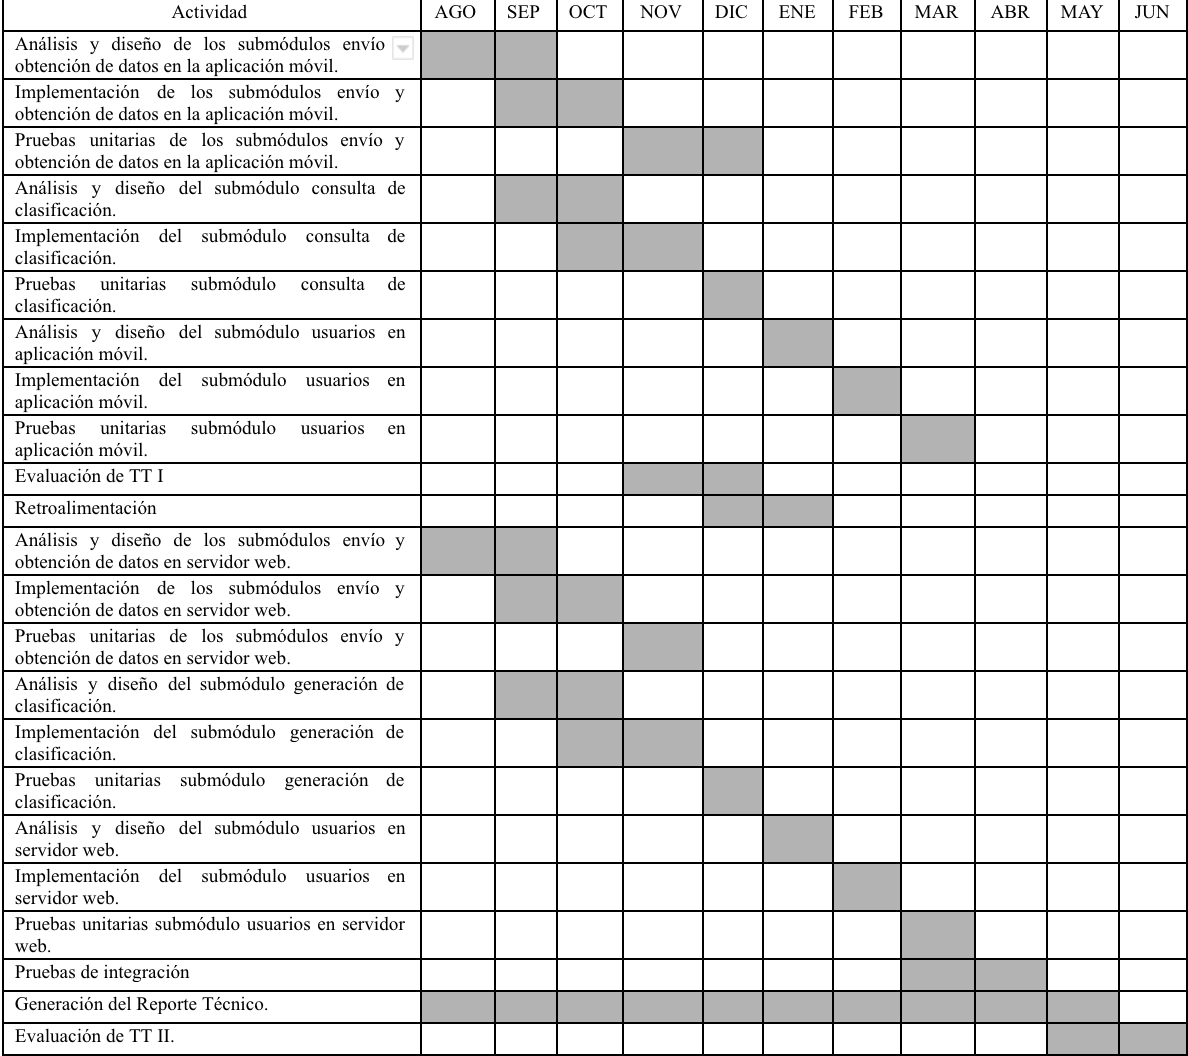
\includegraphics[width=1\textwidth]{Apendice1/cronogramas/batiz}
	\caption{Cronograma de Castillo Reyes Juan Daniel}
	\label{fig:cronograma_batiz}
\end{figure}
\subsection{Monroy Martos Elioth}
El cronograma del alumno se muestra en la Figura \ref{fig:cronograma_elioth}.
\begin{figure}[H]
	\centering
	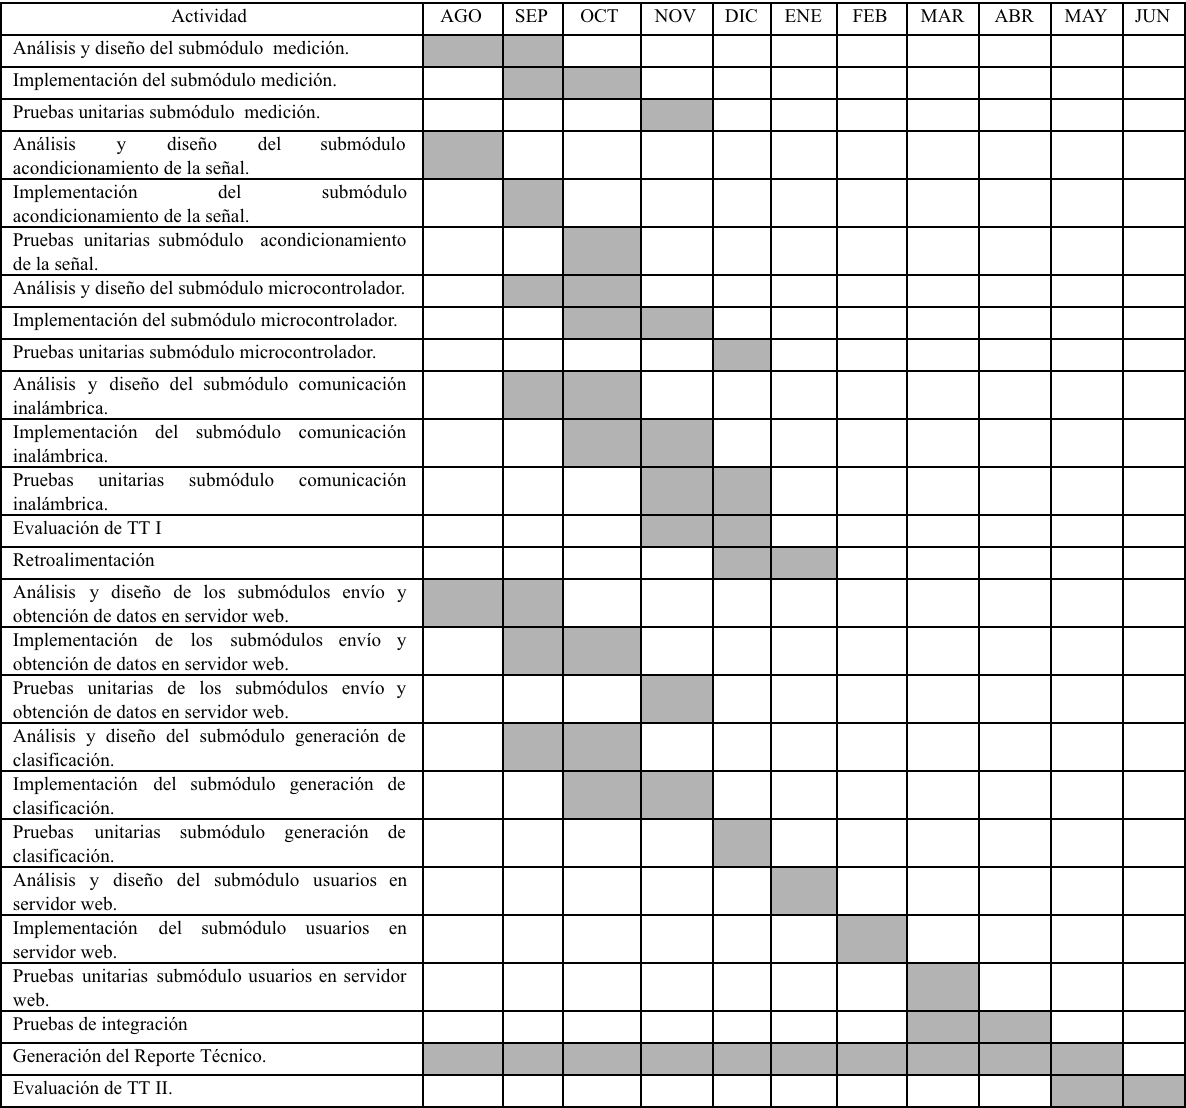
\includegraphics[width=1\textwidth]{Apendice1/cronogramas/elioth}
	\caption{Cronograma de Monroy Martos Elioth}
	\label{fig:cronograma_elioth}
\end{figure}
\subsection{Naranjo Miranda Javier Said}
El cronograma del alumno se muestra en la Figura \ref{fig:cronograma_said}.
\begin{figure}[H]
	\centering
	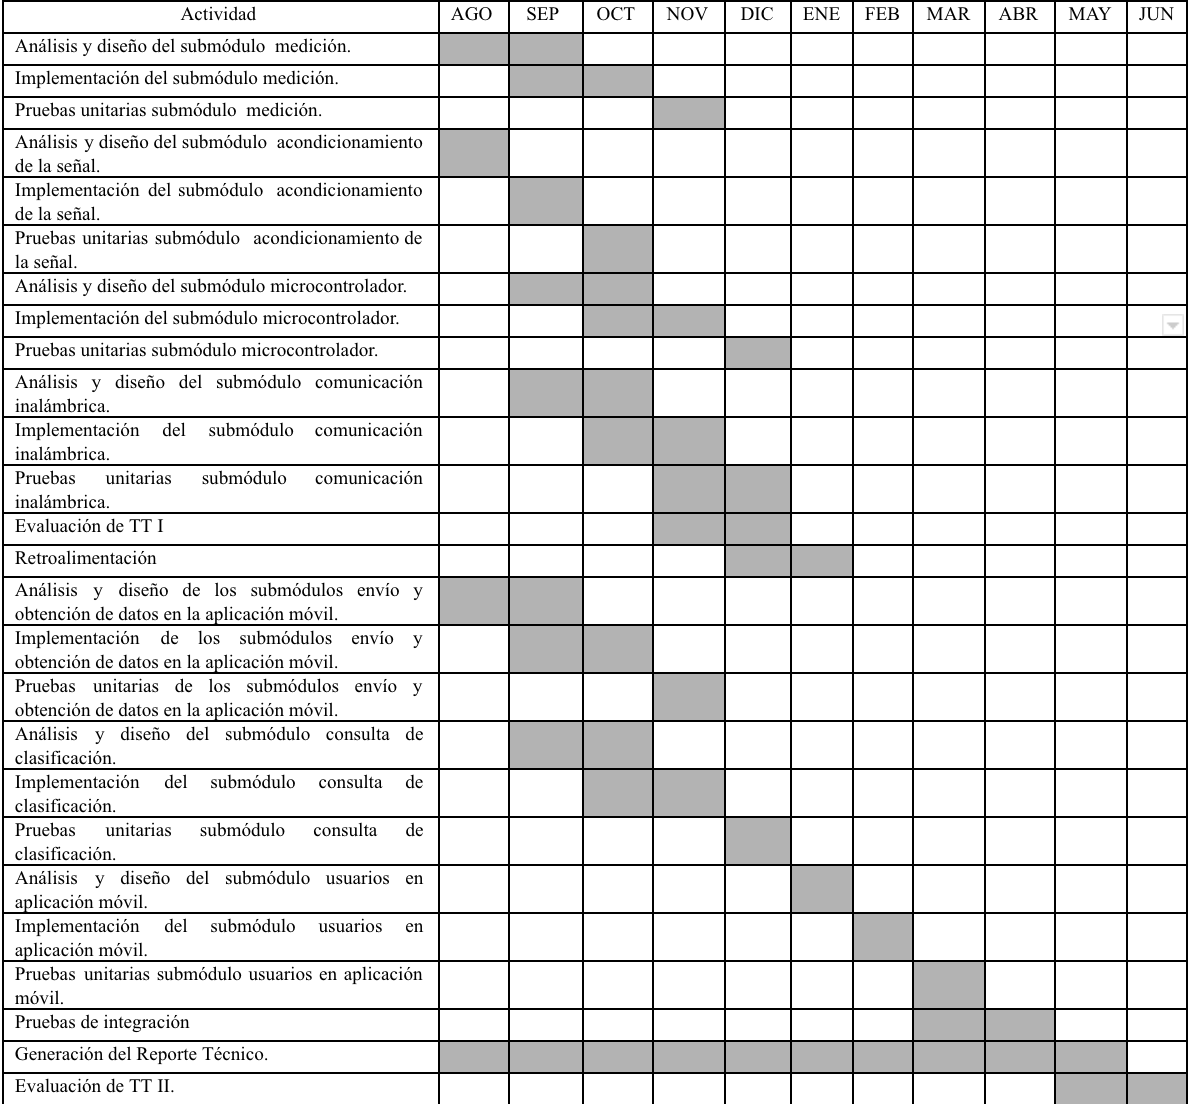
\includegraphics[width=1\textwidth]{Apendice1/cronogramas/said}
	\caption{Cronograma de Naranjo Miranda Javier Said}
	\label{fig:cronograma_said}
\end{figure}
\section{Cambios en los cronogramas de actividades}
A continuación, se presentan los cambios realizados en el cronograma entregado durante el inicio del Trabajo Terminal (protocolo). Las subsiguientes secciones se dividen en cada uno de los integrantes del trabajo y las correcciones que hubo en sus cronogramas.
\subsection{Castillo Reyes Juan Daniel}
\begin{itemize}
	\item La actividad \textit{Pruebas unitarias y submódulo comunicación inalámbrica} fue eliminada debido a que está actividad fue designada a \textit{Monroy Martos Elioth} y \textit{Naranjo Miranda Javier Said}. Permitiendo así que, \textit{Castillo Reyes Juan Daniel} pudiera enfocarse a otras actividades relacionadas mayormente con el desarrollo del servidor web y la aplicación móvil.
	\item La actividad \textit{Evaluación de TT I} fue reacomodada para una mejor lectura del cronograma.
	\item La actividad \textit{Retroalimentación} fue añadida debido a los posibles cambios que pueden ser señalados por los Profesores Sinodales después de la Presentación de Trabajo Terminal I.
\end{itemize}
\subsection{Monroy Martos Elioth}
\begin{itemize}
	\item La actividad \textit{Retroalimentación} fue añadida debido a los posibles cambios que pueden ser señalados por los Profesores Sinodales después de la presentación de Trabajo Terminal I.
	\item Las actividades \textit{Análisis y diseño del submódulo acondicionamiento de la señal}, \textit{Implementación del submódulo acondicionamiento de la señal} y \textit{Pruebas unitarias submódulo acondicionamiento de la señal} fueron eliminadas debido a que el sensor y el microcontrolador seleccionados para la realización del Trabajo Terminal no requieren de un acondicionamiento de la señal (véanse las secciones \ref{sec:Sensor} y \ref{sec:micro}). Esto debido a que el voltaje que arroja el sensor es menor a 5 volts y el microcontrolador soporta como entrada el voltaje que manda el sensor.
\end{itemize}
\subsection{Naranjo Miranda Javier Said}
\begin{itemize}
	\item Las fechas de la actividades \textit{Análisis y diseño del submódulo medición}, \textit{Implementación del submódulo medición}, \textit{Pruebas unitarias submódulo medición}, \textit{Análisis y diseño del submódulo microcontrolador}, \textit{Implementación del submódulo microcontrolador}, \textit{Pruebas unitarias submódulo microcontrolador}, \textit{Análisis y diseño del submódulo comunicación inalámbrica}, \textit{Implementación del submódulo comunicación inalámbrica} y \textit{Pruebas unitarias del submódulo comunicación inalámbrica} fueron corregidas debido a que se encontraban en desorden, en general las fechas de las actividades fueron desplazadas una fila hacía arriba.
	\item La actividad \textit{Retroalimentación} fue añadida debido a los posibles cambios que pueden ser señalados por los Profesores Sinodales después de la presentación de Trabajo Terminal I.
	\item Las actividades \textit{Análisis y diseño del submódulo acondicionamiento de la señal}, \textit{Implementación del submódulo acondicionamiento de la señal} y \textit{Pruebas unitarias submódulo acondicionamiento de la señal} fueron eliminadas debido a que el sensor y el microcontrolador seleccionados para la realización del Trabajo Terminal no requieren de un acondicionamiento de la señal (véanse las secciones \ref{sec:Sensor} y \ref{sec:micro}). Esto debido a que el voltaje que arroja el sensor es menor a 5 volts y el microcontrolador soporta como entrada el voltaje que manda el sensor.
\end{itemize}
\section{Atraso en las actividades de los cronogramas}\label{anexo:atraso}
Durante la realización del presente trabajo, se sufrió un atraso en algunas de las actividades marcadas en los cronogramas. Las actividades afectadas fueron:
\begin{itemize}
	\item \textit{Análisis y diseño de los submódulos envío y obtención de datos en servidor web}: Atraso de 3 semanas debido a que al momento de establecer la arquitectura del sistema (microservicios), fue necesario realizar una investigación sobre las posibles arquitecturas y posteriormente aprender sobre la arquitectura seleccionada, lo cual impedía que se pudiera realizar un diseño y análisis de este módulo, al igual que causó un atraso en las actividades relacionadas con el servidor web como: \textit{Implementación de los submódulos envío y obtención de datos en servidor web}, \textit{Pruebas unitarias de los submódulos envío y obtención de datos en servidor web}, \textit{Análisis y diseño del submódulo consulta de clasificación}, \textit{Implementación del submódulo consulta de clasificación}, \textit{Pruebas unitarias submódulo consulta de clasificación}, \textit{Análisis y diseño del submódulo usuarios en aplicación móvil}, \textit{Implementación del submódulo usuarios en aplicación móvil}, \textit{Pruebas unitarias del submódulo usuarios en aplicación móvil}, \textit{Análisis y diseño del submódulo usuarios en servidor web}, \textit{Implementación del submódulo usuarios en servidor web}, \textit{Pruebas unitarias del submódulo usuarios en servidor web}.
	\item Las actividades \textit{Implementación del submódulo medición}, \textit{Pruebas unitarias submódulo medición}, \textit{Implementación del submódulo microcontrolador}, \textit{Pruebas unitarias submódulo microcontrolador}, \textit{Implementación del submódulo comunicación inalámbrica}, \textit{Pruebas unitarias submódulo comunicación inalámbrica} sufrieron un atraso de un mes, debido a que el sensor de flujo a usar, tardo un mes más en llegar de lo esperado.
\end{itemize}
\section{Encuesta} \label{FactibilidadOperativa}
\textbf{Gasolimetro}
\\Se lanzará al mercado una aplicación móvil que permite conocer las gasolineras que cargan con mayor exactitud el combustible solicitado por el usuario. El sistema consta de un sensor que permite medir el flujo de gasolina introducido en el vehículo.
La siguiente encuesta nos ayudará a medir los niveles de aceptación del producto. La información proporcionada solo se utilizara para fines estadísticos.
\\
\begin{enumerate}
	\item Edad: \\ a.-16 a 20 años\hspace{1cm}b.-21 a 30 años\hspace{1cm}c.-31 a 40 años\hspace{1cm}d.-mas de 40 años
	\item Delegación: \rule{20mm}{0.1mm}
	\item Ocupación:\\ a.-Estudiante\hspace{1cm}b.-Profesionista\hspace{1cm}c.-Empleado\hspace{1cm}d.-Independiente
	\item ¿Con qué tipo de automóvil cuenta?\\ a.-De combustión\hspace{1cm}b.-Híbrido\hspace{1cm}c.-Eléctrico\hspace{1cm}d.-No tengo auto
	\item ¿Qué tan seguido carga gasolina?:\\ a.-más de 3 veces por semana\hspace{1cm}b.-2 o 3 veces por semana\hspace{1cm}c.-1 vez a la semana\hspace{1cm}d.-No cargo gasolina
	\item En promedio ¿Cuánto carga de gasolina?(En pesos)\\más de \$500 \hspace{1cm}b.-Entre \$300 y \$500\hspace{1cm}c.-Entre \$100 y \$300 \hspace{1cm}d.-menos de \$100
	\item Del 1 al 5, donde 1 es poco y 5 es mucho ¿Con qué precisión considera que le cargan litros completos? \rule{20mm}{0.1mm}
	\item ¿Actualmente utiliza algún medio para medir los litros que le cargan?\\ a.-Si\hspace{1cm}b.-No
	\item Pensando en la descripción del producto y en los beneficios que este ofrece ¿Qué tan interesante le parece el producto?
	\\ a.-Muy interesante\hspace{1cm}b.-Interesante\hspace{1cm}c.-Poco interesante\hspace{1cm}d.-No me interesa
	\item ¿Cuánto considera que es un precio adecuado para su venta?
	\\ a.-menos de \$300 \hspace{1cm}b.-Entre \$300 y \$500 \hspace{1cm}c.-Entre \$500 y \$800 \hspace{1cm}d.-mas de \$800
	\item ¿En qué sistema operativo le gustaría que este producto estuviera a la venta?\\ a.-Android\hspace{1cm}b.-IOS\hspace{1cm}c.-Windows Phone
	\item ¿Qué tan útil le resulta este producto?\\ a.-Muy útil\hspace{1cm}b.-Útil\hspace{1cm}c.-Poco útil\hspace{1cm}d.-Nada útil
	\item En una escala del 1 al 5, donde 1 es poco y 5 es mucho ¿Qué probabilidad hay de que consuma este producto?\rule{20mm}{0.1mm}
\end{enumerate}
\section{Resultados de la Encuesta}
A continuación se muestran los resultados de la encuesta.
\begin{enumerate}
	\item \begin{figure}[H]
		\centering
		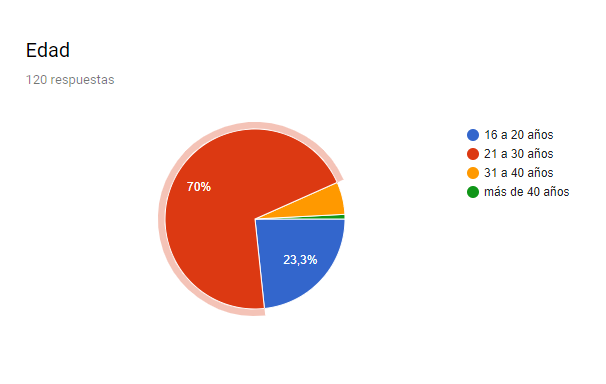
\includegraphics[width=0.5\textwidth]{Apendice2/img/Edad}
		\caption{Resultado pregunta 1}
	\end{figure}
\item \begin{figure}[H]
	\centering
	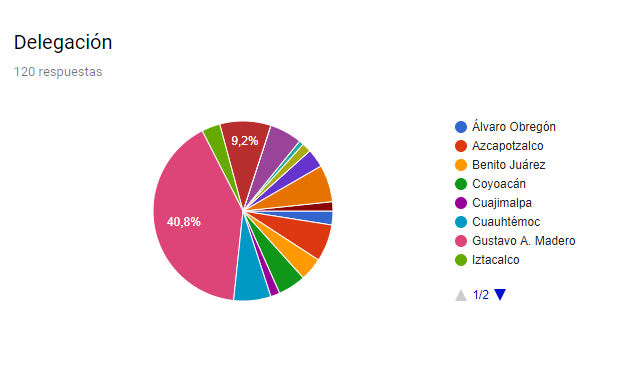
\includegraphics[width=0.5\textwidth]{Apendice2/img/Delegacion}
	\caption{Resultado pregunta 2}
\end{figure}
	\item \begin{figure}[H]
		\centering
		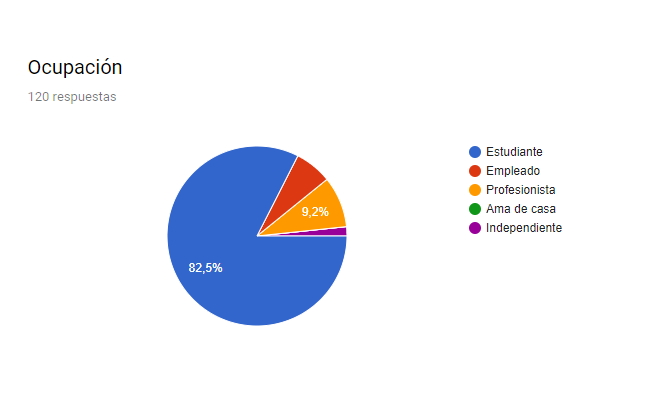
\includegraphics[width=0.5\textwidth]{Apendice2/img/Ocupacion}
		\caption{Resultado pregunta 3}
	\end{figure}
\item \begin{figure}[H]
	\centering
	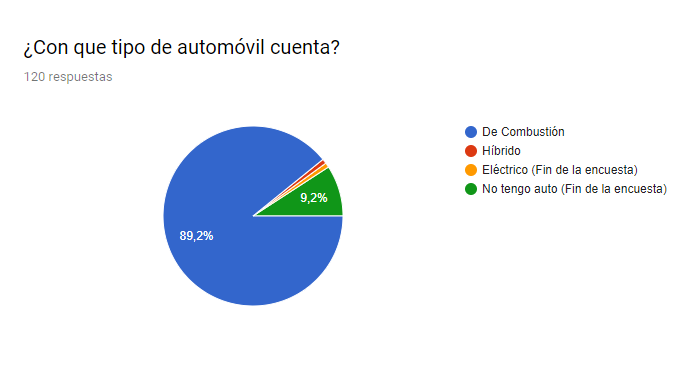
\includegraphics[width=0.5\textwidth]{Apendice2/img/TipoAutomovil}
	\caption{Resultado pregunta 4}
\end{figure}
\item \begin{figure}[H]
	\centering
	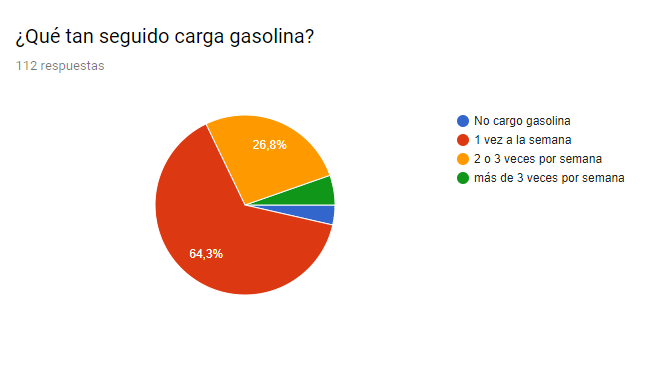
\includegraphics[width=0.5\textwidth]{Apendice2/img/FrecuenciaGasolina}
	\caption{Resultado pregunta 5}
\end{figure}
\item \begin{figure}[H]
	\centering
	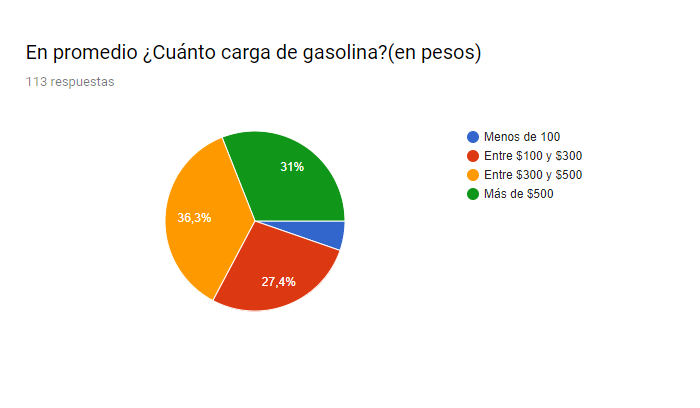
\includegraphics[width=0.5\textwidth]{Apendice2/img/CargaGasolina}
	\caption{Resultado pregunta 6}
\end{figure}
\item \begin{figure}[H]
	\centering
	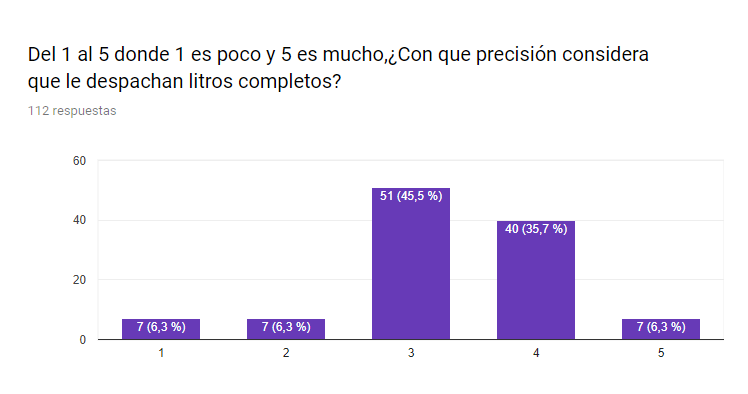
\includegraphics[width=0.5\textwidth]{Apendice2/img/Precision}
	\caption{Resultado pregunta 7}
\end{figure}
\item \begin{figure}[H]
	\centering
	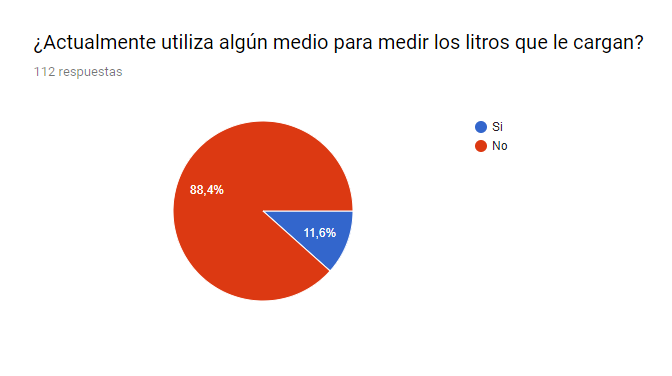
\includegraphics[width=0.5\textwidth]{Apendice2/img/Metodo}
	\caption{Resultado pregunta 8}
\end{figure}
\item \begin{figure}[H]
	\centering
	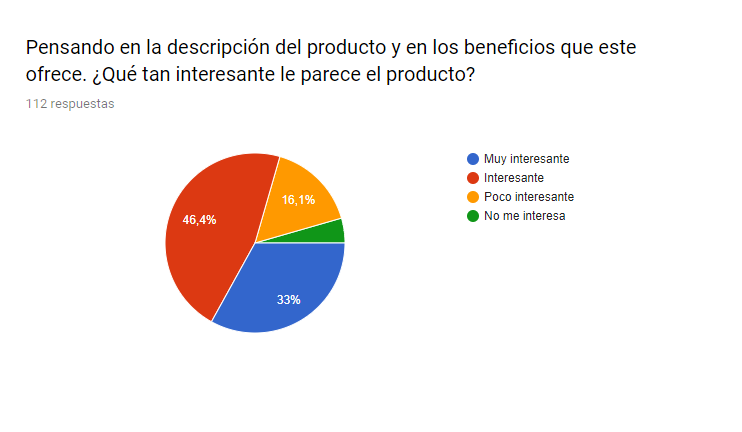
\includegraphics[width=0.5\textwidth]{Apendice2/img/Interesante}
	\caption{Resultado pregunta 9}
\end{figure}
\item \begin{figure}[H]
	\centering
	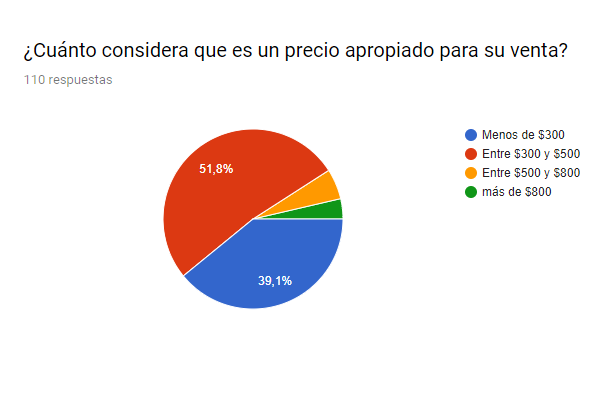
\includegraphics[width=0.5\textwidth]{Apendice2/img/Precio}
	\caption{Resultado pregunta 10}
\end{figure}
\item \begin{figure}[H]
	\centering
	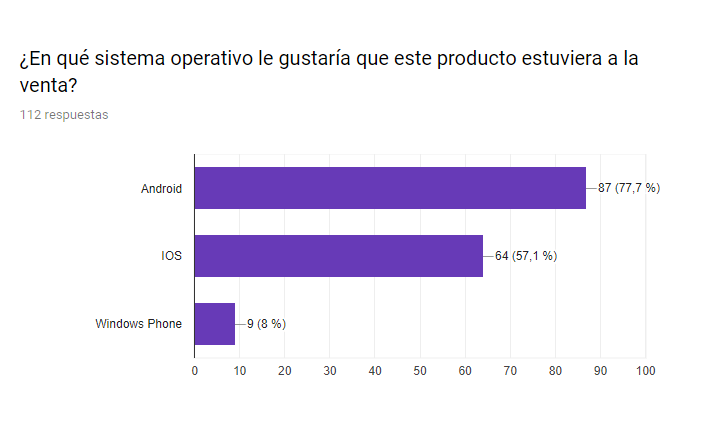
\includegraphics[width=0.5\textwidth]{Apendice2/img/SO}
	\caption{Resultado pregunta 11}
\end{figure}
\item \begin{figure}[H]
	\centering
	\includegraphics[width=0.5\textwidth]{Apendice2/img/Util}
	\caption{Resultado pregunta 12}
\end{figure}
\item \begin{figure}[H]
	\centering
	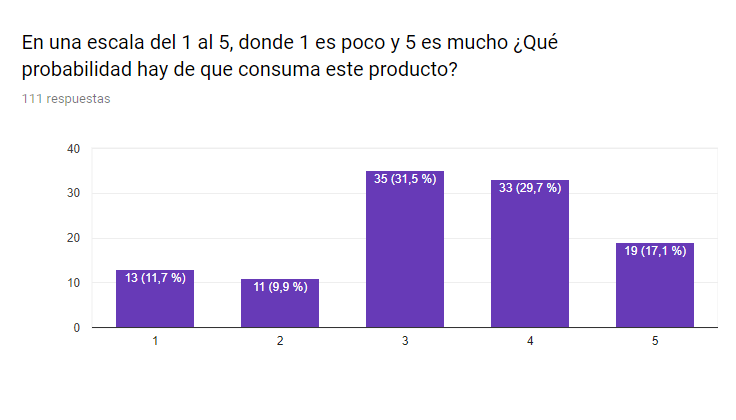
\includegraphics[width=0.5\textwidth]{Apendice2/img/Consumir}
	\caption{Resultado pregunta 13}
\end{figure}

\end{enumerate} 

               % Colocar los circuitos, manuales, código fuente, pruebas de teoremas, etc.
%%%%%%%%%%%%%%%%%%%%%%%%%%%%%%%%%%%%%%%%%%%%%%%%%%%%%
%                   REFERENCIAS                     %
%%%%%%%%%%%%%%%%%%%%%%%%%%%%%%%%%%%%%%%%%%%%%%%%%%%%%
% existen varios estilos de bilbiografía, pueden cambiarlos a placer
\bibliographystyle{ieeetr} % otros estilos pueden ser abbrv, acm, alpha, apalike, ieeetr, plain, siam, unsrt

%El formato trae otros estilos, o pueden agregar uno que les guste:
%\bibliographystyle{Latex/Classes/PhDbiblio-case} % title forced lower case
%\bibliographystyle{Latex/Classes/PhDbiblio-bold} % title as in bibtex but bold
%\bibliographystyle{Latex/Classes/PhDbiblio-url} % bold + www link if provided
%\bibliographystyle{Latex/Classes/jmb} % calls style file jmb.bst

\bibliography{Bibliografia/referencias}             % Archivo .bib


\end{document}
